\documentclass[phd,tocprelim]{cornell}
%
% tocprelim option must be included to put the roman numeral pages in the
% table of contents
%
% The cornellheadings option will make headings completely consistent with
% guidelines.
%
% This sample document was originally provided by Blake Jacquot, and
% fixed up by Andrew Myers.
%
%Some possible packages to include
\usepackage{graphicx,pstricks}
\usepackage{graphics}
\usepackage{moreverb}
\usepackage{subfigure}
\usepackage{epsfig}
\usepackage{hangcaption}
\usepackage{txfonts}
\usepackage{palatino}
\usepackage{url}
%\usepackage{subfig}
\usepackage{verbatim}

%\renewcommand{\comment}[1]{}


%if you're having problems with overfull boxes, you may need to increase
%the tolerance to 9999
\tolerance=9999

\bibliographystyle{plain}
%\bibliographystyle{IEEEbib}

\renewcommand{\caption}[1]{\singlespacing\hangcaption{#1}\normalspacing}
\renewcommand{\topfraction}{0.85}
\renewcommand{\textfraction}{0.1}
\renewcommand{\floatpagefraction}{0.75}

\title {The Dynamics of Information Diffusion on On-line Social Networks}
\author {Shaomei Wu}
\conferraldate {August}{2012}
\degreefield {Ph.D.}
\copyrightholder{Shaomei Wu}
\copyrightyear{2012}

\begin{document}

\maketitle
\makecopyright

\begin{abstract}
Although there has been a long history of studying the diffusion of information in various social science fields, existing theories are mostly built on direct observations in small networks or survey responses from large samples. As a result, it is hard to verify or refute these theories empirically on a large scale. In recent years, the abundance of digital records of online interactions has provided us for the first time both the explicit network structure and detailed dynamics, supporting global-scale, quantitative study of diffusion in the real world. Using these large scale datasets collected from social media sites, this thesis is to mainly address the following three questions about the process of information diffusion: ``who influence whom?'',  ``how do different types of information spread?'',  and ``how does the network structure impact the diffusion process?'' 
%To better understand influence in a hybrid communication channel such as Twitter,

To understand how influence migrates across mediums, we study user's influence on social media based on their role in the global media ecosystem. By categorizing Twitter accounts into elite (i.e. celebrities, media outlets, organizations, and bloggers) and ordinary users, we find a striking concentration of attention on a minority of elite users, and significant homophily within elite categories. On the other hand, following the definition of ``opinion leaders'' in the classical ``two-step flow'' theory, we find a large population of opinion leaders who serve as a layer of intermediaries between the elite users and the masses. 

In contrast to previous diffusion research on the virality of information, our work focuses on the persistence of information, in relation to people and content. Fist, we see a systematical difference, in lifespan, for information broadcase by different categories of users. Second, we find a strong association between the content and the temporal dynamics of information: rapidly-fading information contains significantly more words related to negative emotion, actions, and more complicated cognitive processes, whereas persistent information contains more words related to positive emotion, leisure, and lifestyle.
 
In the end, we study the local and global structure of a decaying online social network. Although there is a significant correlation in both arrival and departure among friends, we show that the dynamics of departure behave differently from the dynamics of arrival. 
In particular, for the majority of users with a sufficient number (e.g., greater than 20) of friends, departure is best predicted by the overall fraction of activity within a user��s neighborhood, independent of size. We also find that active users tend to belong to a core that is densifying and is significantly denser than the inactive users, and the inactive set of users exhibit a higher density and lower conductance than the degree distribution alone can explain. These two aspects suggest that nodes at the fringe are more likely to depart, and therefore induce inactive and subsequent departure of neighboring nodes in tightly-knitcom-munities.


\end{abstract}

\begin{biosketch}
%Your biosketch goes here. Make sure it sits inside the brackets.
\end{biosketch}

\begin{dedication}
%This document is dedicated to all Cornell graduate students.
\end{dedication}

\begin{acknowledgements}
Many many many thanks to my committee!
%First, I would like to thank my advisory committee - Michael Macy, Jon Kleinberg, Dan Cosley - for all the mentoring during my PhD study.
%Thanks to my advisors Michael Macy, Jon Kleinberg, Dan Cosley. Many thanks to Duncan Watts, Jake Hofman, Winter Mason and everyone from Yahoo Resarch. Thanks to Andrew Tomkins and Google Research. Thanks to Ben Lickly, Shenwei Liu, Patrick Park, Yongren Shi, Chris Cameron, Tim Novikoff, Johan, Daniel, Jure for discussion. Thanks for Hyunyong, Karin, Theresa, Yookyung for always offering good insights. Thanks to my family for supporting!!!

\end{acknowledgements}

\contentspage
\tablelistpage
\figurelistpage

\normalspacing \setcounter{page}{1} \pagenumbering{arabic}
\pagestyle{cornell} \addtolength{\parskip}{0.5\baselineskip}

%\part{Introduction and Background}

\chapter{Introduction}
%With the invention of print, telephone, the Internet, the amount of information a person can 
%However cynical Postman is, he has made a point that medium has an effect on both the form of information and the way it is disseminated and processed. Through the evolution of communication technology, information has become more and more easier to be produced, faster to be propagated, and more accessible.

%With the huge IPO of FB and the great pontential expected from Twitter, social media and social marketing have become the new silicion valley favorite and created a new wave of glamous bubbles.

Information diffusion has been a long intriguing topic for scholars from different fields. It is an essential element of many interesting problems, such as the diffusion of innovation\cite{rogers-2003}, formation of public opinion\cite{katz_lazarsfeld,Watts-2007}, adoption of new products\cite{Bass:1969}. Historically, most of the research in this area has been done through field observations and/or phone surveys\cite{katz_57,rogers-2003}. Confined by the methodology, their results are uaually based on the spread of a specific opinion or product in rather localized networks. 

The development of the Internet and the emergence of a whole new set of communication technologies on top of it has largely changed the way people  gather and disseminate information, and brought both challenge and opportunity to a better understanding of how information spreads in the society.
Historically, most empirical studies in this area were based on data collected through in-person interviews and phone surveys\cite{rogers-2003,katz_lazarsfeld}, targeted with a specific opinion or product that is under diffusion. Confined by the methodology, theories and conclusions drew from these research suffer at scale and data accuracy, and are challenged in today's massive, hybrid communication environment. Meanwhile, the popularity of eletronic communication tools has offered new possibilities for obtaining much better data on how information and behavior spread over large population. The abundance of digital records of online interactions can provide large amounts of data on both explicit network structure and detailed dynamics, supporting large-scale, quantitative study of diffusion in the real world.

Using these large scale datasets collected from social media sites (i.e. Twitter, Orkut), we study three major components of information diffusion process:
\begin{itemize}
\item \emph{People}, who are the ``influentials'' and whom are they influencing?
\item \emph{Content}, does different types of information spread differently?
\item \emph{Network}, what can the macro- and micro-level structure of the network tell us about the underlying mechanism that drives the diffusion process?
\end{itemize}

Although still a young field, there has been a growing literature that studied these components, mostly focused on modeling and predicting the scale or the spikiness of cascade. Building on top of existing knowledge, our exploration on these three components highlights the following three contributions:

%In this thesis, I will discuss our exploration on these three components of diffusion, highlighting our contributions on the following three aspects.

%Built on top of existing research, this thesis will contribute our knowledge about the dynamics of information diffusion on online social networks, from three perspectives.

First, we study the ``virality'' of diffusion with new aspects. Instead of scale, we focus on the temporal patterns of cascades, in particular, the persistence of information. We notice that certain information has a very long lifespan whereas most of the information only exists shortly in social media. We also look at the ``negative'' virality - the virality of ``inactivity'', and show how user disengagement, similar to user engagement, has a network effect but operates slightly differently.

Second, we examine the exogenous properties of actors and artifacts beyond the closed, single-medium communication network. For example, by looking in-depth at the textual characteristics, we find that the persistent attention to certain content can be better explained by the innate quality of the content, independent from the mechanism of how it spreads in the network. We also find that, despite the connectivity and demographics, certain users are more influential on social media because of their established role (and fame) from the world outside social media. These results suggest that, diffusion process should be studied in context, considering the socio-cultural factors that constantly interact with the information cascade.

%Our results show that, diffusion should be studied in context, taking into account the socio-cultural factors that constantly interact with the diffusion process. 
%These findings suggest that, online social networks are not isolated systems, but instead, a part of the global communication networks with many existing channels, actors, and communication artifacts.

Third, we study different components of diffusion not only by themselves, but also the interaction between them. As information diffusion is an interactive process between people and content, mediated by the communication networks, different components of diffusoin do not exist in isolation. People with high influence tend to cluster together\cite{Aral-2012}, and the location in the network can tell us a lot about a person's status\cite{Kempe-2003,Backstrom:2006}. In our work, we show that different people have different preference of content and invididual's influence is topic-dependent.

%In the end, we will examine a diffusion process that closely tight the online and offline world together - Arab spring. Contributions:
%\begin{enumerate}
%\item Trace the evolution, and unveal the dynamicss of social movement using digital logs;
%\item Understand the role and impact of social media in societal changes;
%\end{enumerate}

This thesis is an inter-disciplinary effort. Although most of the results are quantitative and are drew from analysis on large online datasets, I have worked closely with experts from various fields including sociologists, computer scientists, phycologists, communication scholars, and political scientists. During this process, I try to conduct my research with not only computational methods but also theories and insights from different fields. As a result, I hope our findings are not limited to online social networks, but can also help uncover the nature of information diffusion process acorss online and offline spaces.

%Finally, we study the arab spring movement and hope that the insights from our work is not limited to online social networks but also help uncover the nature of information diffusion process across online and offline environement.

\section{The predictability of virality}

With viral videos and memes outbreak and circulating in the Internet almost everyday, brands and politicians are eager to leverage the power of social networks and run online campaigns that ``go viral''. The demand from the market, contrasted with our lack of knowledge on the mechanism behind viral phenomenons, has catalyzed many studies focusing on modeling and predicting the virality of diffusion process. In this line of work, virality is usually defined and measured in three aspects: 
\begin{enumerate}
\item \emph{Scale}: the size of cascade tree originated from the original node. e.g., the cascade Facebook fanning pages;
\item \emph{Range}: the maximal chain length in the diffusion network. e.g., blog\cite{Leskovec-SDM-07}. 
\item \emph{Transmission probability}. As most existing research describe diffusion process with epidemic models, transmission probability is the probability a virus travels through a directional edge in the network and infects the end node. In the context of social networks, transmission probability is mapped to  the success rate of interpersonal recommendations in electronic market\cite{Leskovec-EC-2006}, the probability a tweet is retweeted by the followers of the tweet's author\cite{Bakshy-2011}, and the likelihood a user mark a Flickr photo as favorite after seeing a friend doing so\cite{Cha-2009}.
\end{enumerate}

Using large scale online social networks data, researchers have employed a whole set of computational tools to asset different aspects of cascades that may lead themselves to viral. However, in practice, it is still very difficult to engineer a success viral campaign\cite{Bakshy-2011}. In fact, most marketers and public relation professionals still rely heavily on experience and intuition when launching online campaigns, which mostly received attention in a short timespan\cite{Jaewon-2011,crane:2008,Wu-ICWSM-2011,Wu-Twitter-2011}. Although the virality is still the holy grail for marketers, there has been an ascending suspicion on the whole idea of ``predicting virality''.

In their Science article published in 2006, Salganik et al\cite{Salganik-2006} explored the unpredictability of song ratings, argued that, despite the quality of music, the best predictor for a song's popularity is actually the popularity itself: the songs that received first few thumbs-ups usually rise up to be the hit, even if the first thumbs-ups are given randomly. Some later work showed that the quality of initiators does not predict well with the final scale of cascades\cite{Sun-2009,Bakshy-2011}. Although some studies showed that the structure of the subgraph induced by existing adopters do have a role in behaviro adoption\cite{Backstrom:2006,Romero-2011,Leskovec-SDM-07}, such role is not consistent in other studies\cite{Bakshy-2011}, and may depend on the context of diffusion\cite{Centola:2007}.

There are two major factors that might contribute to the difficulty of predicting virality. First, as most studies observed, the power-law (or log-normal) distribution of the popularity of online content results in a skewed training set consisting of many unsuccessful examples and only a few successful examples. While most machine learning algorithms are not robust to skewed training sets\cite{Provost-2000}, the common practice of biased sampling can over-compensate the successful cases and overlook the unsuccessful ones. As a result, most characteristics we discovered in the positive class can also be found in the negative class - the predictive model would fail to tell one from the other. Second, as we mentioned before, given the fact that online communications is an integrated part of the global communication networks, there are many exogenous factors that can not be controlled or observed in the communication channel where the data is collected. The complexity and the fuzziness of real world diffusion process is innately inadequate to be fully captured by epidemic models\cite{Bakshy-2011,Cha-2010}.

Understanding the difficulty of this task does not mean that it is unsolvable. We have seen tremendous progress towards a better understanding of the virality, incorporting theories and methods from multiple fields (e.g., \cite{Centola:2007, Bakshy-2011}). As part of these efforts, we also study the \emph{transmission probability} of URLs among different categories of users on Twitter. Our results show that influential users are much more likely to pass on information from those who are similar to them (for more details, see Chapter~\ref{chap:influece}).

Meanwhile, during our study of the spread of URLs on Twitter, we discovered and explored some new metrics for the success of cascade. We first noticed that,  although skewed as well, the distribution of the lifespan of information has a much heavier tail towards the end. In other words, there is a substantial amount of information that is consistently tweeted over a long period of time, in the fast-paced medium such as Twitter. When examining the persistent items in depth, we realized that, most of them can not be characterized by any of the traditional metrics for virality: they do not receive many retweets, they do not spread through long-chains, and they are usually not part of super-sized cascades. However, as they generate comparably large interest that lasts for a signficantly long period of time, we believe that persistent content are interesting enough to be studied as ``success'' examples of diffusion as well.

The study of information longevity is generally missed in the study of information diffusion, even among the string of research on the temporal dynamics of cascades\cite{Yang-2011,crane:2008,Leskovec:2005}. Although some previous work also spotted the lastiningness of certain content\cite{crane:2008,Szabo-2010}, researchers usually concentrate on modeling the speed, intensity, and scale of the peak of attention, while treating the long-last content as corner cases.
%Although there has been a growing interst at studying the temporal dynamics of diffusion process\cite{Yang-2011,and others}, most work has concentrated on the peak of attention, but not the longevity. %studying how fast the peak is accumulated\cite{}, how attention are distributed around the peak\cite{}, and how long the cycle is when there are more than one peaks\cite{}. 
%Even in previous work that also spotted the lastingness of certain content\cite{crane:2008,Szabo-2010}, authors were trying to predict the speed and intensity of the burst of attention while treating the long-last content as corner cases. 
In our work, we compare the lifespan of information by its initiator and content, and ask what makes certain things so persistently eye-catching in a world where information is overly rich and attention is remarkably scarce\cite{Simon-1971}. Our major findings include:
\begin{itemize}
\item The longevity of information is determined to a large extent by the exogenous qualities of the information, not by social contagion. 
\item Content picked up by certain group of users (e.g., bloggers) are in general of more persistent interest, as these users actively perform the role of ``information filter'' on online social media.
\item There is a strong correlation between the content and the temporal dynamics of information. Content with cultural/intelligent value are more likely to persist. At the text level, rapidly-fading information cntains signficantly more words related to negative emotion, actions, and more complicated cognitive processes, whereas the persistent information contains more words related to positive emotion, leisure, and lifestyle.
\item The decay of attention, although much less visible, also has a network effect that coordinates the disengagement in online social networks among friends.
\end{itemize}

%Although many work on temporal analysis, and 
%Similar pattern has also been found in the viewing of YouTube videos\cite{crane:2008,Szabo-2010}, most of them concentrated on the peak and intensity, not the longevity.

%``early temporal dynamics is important at predicting the final popularity'' \cite{Szabo-2010}. ``without early temporal dynamics, semantics is important''.

  
%Inspried by the examples of big cascade, and the market buzz, 
%most existing work has focused on modeling and predicting the scale of diffusion (i.e., virality). 

%Two major reasons for the ``unpredictability''.

%First, power law of popularity - large majority of unsuccessl events that are over-looked, and given the number, they pontentially exhibit all characteristics of viral examples.

%We also made efforts on predicting the scale. Then we switch our gear to studying the temporal dynamics of information, following an emerging line of research\cite{}. Patterns they have shown... In current study of temporal dynamics, most work on the trend, and the peaks. However, we start to look at the longevity of information, and ask what makes information persistent. Interestingly, the distribution of lifespan does not follow power-law, but instead, with a large number of items with super long lifespan. When looking these items, we find they can not be characterized by any of the viral metrics above. They are not viral, nor generated by long-chains, and usually not part of big cascade.  However, they are very interesting because... (they are like organic process that does not die!)

%Existing efforts on predicting the popularity with early activity patterns\cite{Szabo-2010}.

%Second, exogenous characterstics - the innate inadequate of epidemic models. When we think to model virality, we need to think in a bigger context (details in following sections).



% Understanding how information spreads in the society has attracted a growing interest from both practitioners and scholars. It is an essential element for many interesting problems, such as the diffusion of innovation, formation of public opinion, product adoption, and viral marketing. 

%Historically, one of the biggest challenges in the study of information diffusion is data collection. Given the difficulty of observing and tracing the diffusion process over all possible channels, most empirical studies in this field have been conducted manually by sociologists and communication researchers, through in-person interviews or standardized surveys of population samples. Therefore, these studies are largely confined by the scale and the data accuracy. As a result, existing theoretical models in the literature have relied on many assumptions about the underlying diffusion mechanism instead of empirical evidence. Being widely applied, these models are, however, hard to be verified or rebutted empirically on a large scale. 

%In recent years, the abundance of digital records of online interactions has provided us both the explicit network structure and detailed dynamics, supporting global-scale, quantitative study of diffusion in the real world. 

%Using these large scale datasets collected from social media sites (i.e. Twitter, Orkut), this thesis addresses the following three questions: ``who influences whom?'', ``how do different types of information spread?'',  and ``how does the network structure impact the diffusion process?''

%Viewing the diffusion of information as an organic process, we study each stage in its lifecycle, from production, dissemination, to consumption (deceased). Each part is motivated by social science problems and theories, and aim at contribute deeper insights about how information flow in the society and its impact.

%our work mainly contributed to the aspectes in the lifecycle of information diffusion that are overlooked by previous studies:
%\begin{enumerate}
%\item Production: people's external influence, especially, the role of mass media
%\item Dissemination: temporal dynamics and the role of content
%\item End-of-life: how does disengagement happen?
%\end{enumerate}


%\begin{enumerate}
%\item Production: what can we know about the diffusion when the information is created - persistance (compared with the seed selection problem);
%\item Dissemination: influencers, content, network structure, and the interaction among them.
%\item End-of-life: network effect on disengagement.
%\end{enumerate}


\section{The Influencer Problem}

%These tastemakers, Gladwell concluded, are the spark behind any successful trend. "What we are really saying," he writes, "is that in a given process or system, some people matter more than others." In modern marketing, this idea--that a tiny cadre of connected people triggers trends--is enormously seductive. It is the very premise of viral and word-of-mouth campaigns: Reach those rare, all-powerful folks, and you'll reach everyone else through them, basically for free. Loosely, this is referred to as the Influentials theory, and while it has been a marketing touchstone for 50 years, it has recently reentered the mainstream imagination via thousands of marketing studies and a host of best-selling books. In addition to The Tipping Point, there was The Influentials, by marketing gurus Ed Keller and Jon Berry, as well as the gospel according to PR firms such as Burson-Marsteller, which claims "E-Fluentials" can "make or break a brand." According to MarketingVOX, an online marketing news journal, more than \$1 billion is spent a year on word-of-mouth campaigns targeting Influentials, an amount growing at 36\% a year, faster than any other part of marketing and advertising. That's on top of billions more in PR and ads leveled at the cognoscenti.

%Uniqlo - flagship stores in NYC, featuring ``community heros'' such as restaurant owner and street fair organizer.

The role of the influentials as trend makers has been a center piece of many classic theories about information diffusion process\cite{katz_lazarsfeld,rogers-2003}. The existence, and the importance, of the influentials also populated by several best-selling books such as The Tipping Point\cite{Gladwell:2002} and The Influentials\cite{keller_berry}. Today, challenged by the unbounded opportunity (and efforts) to reach the masses, marketers and PR firms are especially eager to leverage the power of the influentials to ``tip'' their products. But, who are the influentials? 
%Can we estimate person influence and pick out the influencers?

There are several classic theories about the characteristics of the influentials. Dating back to the 50s, Katz and Lazarsfeld coined the term ``opinion leaders''. They claimed that, comparing to ordinary people, opinion leaders have more social connections and are more media-savvy\cite{katz_lazarsfeld}. Later, scholars studying the diffusion of innovations also suggested that opinion leaders usually own ``greater exposure to mass media than their followers'', ``are more cosmopolite'', ``have greater social participation'' , ``have higher socioeconomic status'', and ``are more innovative''\cite{rogers-2003}. Similar ideas are illustrated in best-selling books, in which authors claims that the influentials are ``connectors'', ``mavens'', and ``salesmen''\cite{gladwell}, and that influentials play their role actively and constantly, providing suggestions from what to buy to who to vote for\cite{keller_berry}.

One critic to the classic theories is their lack of empirical supports. Although intuitively sound, these theories about influentials are too general to be operationalized or examined in practice. It was only since the abundance of online interaction data that we saw a new line of empirical work on measuring and quantifying personal influence in diffusion. Most of these work studied influence in two aspects: personal attributes such as demographics and activities, network attributes such as connectivity and position in the network.  Although both aspects are usually considered and studied, most work showed the network attributes more relevant to personal influence\cite{Sun-2009,Bakshy-2011,Kempe-2003,kwak_10,Leskovec-EC-2006,Cha-2009}. 

%Many work studied people in different demographics groups and the associated impact in diffusion process. However, although some research showed that age and gender are related with the tendency of adopting a new product\cite{}, most existing work found no siginificant correlation between individuals' demographics and their likelihood of seeding big cascades\cite{Sun-2009,Bakshy-2011}. Instead, people argued, it is the position in the network and the strength of social ties that makes some people more influential than the rest\cite{Kempe-2003,kwak_10,Leskovec-EC-2006,huberman, cha&mislove}. 

However, we find current knowledge on influence and influentials still limited for several reasons. First, as most work focused on big cascades, the results can be biased towards the ``successful'' events that are deemed to be rare\cite{Bakshy-2011}.

In addition, the \emph{context} of influence is usually overlooked. Influence deos not exist in vacumne. It needs to be exercized by people, with certain communication medium. The context of influence is important, because individuals influence can differ by their expertise\cite{Cha-2010}, the subject\cite{Leskovec-EC-2006}, and the communication channels\cite{Wu-Twitter-2011}. Existing empirical studies measure influence in a variety of ways, from the size of diffusion tree, to the probability of passing the cascade to the next hop. The lack of consistency in current definition of influence also introduces ambiguity: different types of influence are usually studied as a whole, regardless different mechanisms that operate behind them. As a result, hybrid influence is observed and studied as if driven by a single mechanism. For example, exogenous influence migrated from other channels is usually mixed with and treated as interpersonal influence in most emiprical studies.

%As a result, homophily can be 

%With any of the exsiting metrics, influence 

%As a result, current definition of influence is not only inconsistent but also ambiguous. Across studies, influence is measured in various ways, from the size of diffusion tree, to the probability of passing the cascade to the next hop. With any of the exsiting metrics, the influence measured is usually driven by a mix effect of social contagion, homophily, and exogenous factors. However, most 

%Several recent research has raised concerns on attributing homophily as social contagion\cite{}, but the exogenous factors are still largely overlooked. 

%Bloggers follow the news threads participate in the news cycle originated by mass media with an amazing regularity. 

%Such inconsistency not only makes it impossible to compare the results across studies, but also introduces the ambiguity in the meaning of influence. 

%As a result, different types of influence are mixed and studied as if driven by a single mechanism.

%As discussed before, in today's hybrid communication environment, the dissemination of information usually happened in multiple channels, driven by a mixed influence from mass media to family and friends. Even in online social media such as Twitter, individual's decision to retweet a message, is usually  

%However, some recent studies have challenged this whole idea about 

%Recently, this idea of networked influence is recently challenged, too. One problem of existing work on this direction is the bias induced by over-sampling the ``successful'' diffusion events that rarely happen in reality\cite{Bakshy-2011}. Another problem is the lack of context in the study of influence. As a result, the definition of influence is inconsistent and ambiguous, makes it hard to compare results across studies or understand the specific mechanism that drives influence of different kinds\cite{Cha-2010,kwak_10,Bakshy-2011}. 


In Chapter~\ref{chap:influece}, we approach the influencer problem by leveraging people's external influence to online social media. Here, we consider online social media as a medium that carries a whole spectum of communications, from personal and private interactions to mass media broadcasting. We thus categorize users based on their role in the global communicaiton system. To eliminate the bias towards successful cascades, we study the influence of each category in terms of visibility and the ability to stimulate and sustain attention from other users. Our work makes three main contributions:
\begin{itemize}
\item We introduce a crowd-sourcing method for classifying users into ``elite'' and ``ordinary'' users according to their role in the media ecosystem, further classifying elite users into one of four categories of interest ��media, celebrities, organizations, and bloggers.
\item We investigate the distribution of attention among these categories, finding that although audience attention is
highly concentrated on a minority of elite users, much of the information they produce reaches the masses indirectly via a large population of intermediaries - local opinion leaders.
\item We find that different categories of users emphasize different types of content, and that content originated by different users exhibit dramatically different characteristic persistency, ranging from less than a day to months.
\end{itemize}


%and hard to be compared across studies. 

%The lack of context can potentitally fraud current 
%Also, most current measurement of influence is measuring a mix of different types of influence driven by differnet mechanisms such as 

%which makes it not only impossible to compare the results across studies, but also hard to articulate the mechanism that drives different types of influence. For example, if the influence is measured by the probability 

%explain what exactly influence means. With most of the metrics (e.g., propagation probability, size of cascade tree, length of induced chain), influence is a 

% Also, as well as the ambiguity between different types of influence\cite{Bakshy-2011}. 

%partly by the potential bias induced by over-emphasizing on rare, successful events, partly by the lack of 

%In fact, computer theorists showed that, given the complete network structure, an approximate algorithm can efficiently select a subset of seeding nodes that maximize the extent of diffusion\cite{Kempe-2003}\footnote{Under the assumption that diffusion process operates as described by the Independent Cascade Model. More details about Independent Cascade Model can be found in Chapter 2.}.

%Although beautifully solved in theory, finding the position of influentials in their social networks is not an easy task in real world. 

%In short, influence is very much context-dependent.


%Sometimes influence is not defined by individual's properties, but by the susceptible their neighbors are\cite{Sun-2009,Watts-2007}.

%Influencers can be found by one's location in the network. Competing theories: centrality, bridging effect, closeness of local community. \cite{mason}
%\cite{Kempe-2003}


%influential individuals are
%less susceptible to influence than non-influential individuals and that they cluster in
%the network, which suggests that influential people with influential friends help
%spread this product.

%Influence by demographic (gender)

%younger users are more susceptible than older users, men are more influential than women, women influence men more than they influence other women, and married individuals are the least susceptible to influence in the decision to adopt the product we studied\cite{}.

%disagreement\cite{Sun-2009,...}

%Influence by tie strength: density of communication, connection to sheepie people.

%Influence based on past performance\cite{Bakshy-2011}.

%All theories incorporated in Klout's algorithm - commercialized but heavily critized.

% The following paragraph is copied pasted from Aral-2012
%In addition to the distinction between local and global signals, it  is important to classify systems into two separate categories based on whether their dynamics are endogenous without external drivers, or exogenous and driven externally, or both. These distinctions are useful because they identify the fundamental characteristics of the system, and hence enable systematic comparisons with other systems. Epidemic spreading in a closed system is an example of an endogenous process with local transmission, because the pathogens need to be passed from one person to another in close physical proximity. Similarly, it is possible to model the spread of innovations such as the uptake of new hybrid crops by farmers as an endogenous social contagion process, and to try to distinguish between different types of local processes that may underlie the observed rate at which the innovation is adopted (26). However, studies of social influence which focus on local and endogenous processes such as word-of-mouth transmission are almost always open to the challenge that they neglect equally important exogenous effects such as marketing or mass advertising, and typically trying to separate these two confounding factors is highly problematic. For instance, a reanalysis (27) of the classic diffusion studies on how prescriptions for an antibiotic drug spread among physicians in different communities (10, 11) suggests that marketing efforts, in this context corresponding to external drivers, can account for most of the observed behavior. Although in general both endogenous and exogenous effects may be present in both online and offline systems, as part of our research design we have identified a system that does not have an exogenous component. Instead, both local and global signals are generated endogenously within the system, that is, there is no exogenous driver. This is in contrast to classic innovation diffusion models (e.g., 28), which feature one rate of contagion from within the group (local signal) and another externally imposed (as opposed to endogenously generated) rate of contagion from outside the group (global signal). Another important feature is that here the user has an active role in deciding whether or not to adopt an application.

%We propose: influence by exogenous status and social roles.
%Think of influence in context:
%\begin{enumerate}
%\item general influence: mass media
%\item domain influence: masspersonal (celebrities, bloggers, organizations)
%\item personal influence: tie strength, content, language, timing (accidental influencers)
%\end{enumerate}

\section{The role of content}
Although it has been a common belief that different types of information spread differently, the role of content in diffusion process has not been examined thoroughly and systematically. Most empirical work in this area focused on the relationship between information virality and content\cite{Berger-2010,Hansen:11}, while some explored the connection between the temporal patterns and the content\cite{Gruhl-2004,crane:2008}. However, these studies are limited either by the lack of observations, or -- when viewed as content-base predictions -- by the relatively weak predictive power. 

%Some studies the temporal patterns.

%Results from these work are general, or lack of predictive power.

There are several major challenges here. First, the content itself is difficult to track, especially when it travles and mutates across multiple media channels over a long period time\cite{Leskovec-Newscycle-2009}.  Second, predicting the virality of information at an individual level is a very hard problem by itself\cite{Bakshy-2011,Szabo-2010}. Third, given the focus of past work on how people interact with information, modeling such dynamics becomes extremely complicated with many unpredictable elements involved\cite{yang-2010,Yang-2011,Wu-Twitter-2011,Bakshy-2011}. 

In Chapter~\ref{chap:content}, we study the relationship between content and temporal dynamics of diffusion on Twitter. 

We tackle the information tracking problem by taking advantage of the URL shorteners (e.g. bit.ly, TinyURL, etc) commonly adopted by Twitter users. Considering each webpage as a unit of information, the URL shortening services tag a page with a unique token that is easily traceable in Twitter communications. As a result, we able able to track the whole lifespan of a specific webpage by the inclusion of the shortened URL in tweets. 

In response to the difficulty of predicting the virality (e.g., scale, tranmission probability), we shift our attention to the persistency of information. We compare two extreme temporal patterns in the decay rate of URLs embedded in tweets, defining a predicting task to distinguish between URLs that fade rapidly following their peak of popularity and those that fade more slowly. Our experiments show a strong connection between content and the temporal dynamics of information.

Also, by studying the webpages instead of individual tweets, we have a much richer, and more static corpus of content that allows us to simplify our model by focusing on the textual content instead of the users, while still maintaining sufficient degree of freedom to generate Another advantage of our approach is that if we can predict the temporal pattern of information based on content alone, we will be able to do that at a very stage, presumably when the information is first generated - which can be of interest to practioners. 

In summary, we study intrinsic qualities of the content that may effectly determine the dissemination process, especially, the persistence of information. Our two main contributions include:
\begin{itemize}
\item We build a classifier that predicts the decay/persistence of information with textual features, providing one of the first empirical studies of the connection between content and temporal variations of information diffusion processes in online social media.
\item We investigate the properties of the text that are associated with different temporal patterns, finding significant differences in word usage and sentiment between rapidly-fading and long-lasting information.
\end{itemize}



%While most existing research studied content under diffusion at the topic level\cite{Leskovec-EC-2006,Romero-2011}, we conduct in-depth text level analysis, looking at the content not only by types but also by its linguistic properties such as sentiment and part of speech.

%Recommendations of different categories of products\cite{Leskovec-EC-2006}.
%temporal dynamics of different content\cite{crane:2008}.
%adoption of different types of Twitter hashtags\cite{Romero-2011}.
%tweets including a hyperlink generates bigger cascade.\cite{yang-2010}
%``semantic analysis of content is useful when no early click-through information is available''\cite{Szabo-2010}

%We found that information with cultural values last long. 

%Individuals are selective at what content they like to read and share.

\section{The network effect of disengagement}
The structure of network is another interesting component of diffusion research. 

At a local level, many studies have shown the correlation of activity among friends in online communities, and tried to understand the effect of neighborhood structure on the spread of information, or behavior. Classic theory on product adoption suggests an ``S-shape'' curve\cite{Bass:1969} in which the probability of adopting a new product grows slowly with a small number of adopted friends $k$, rapidly as $k$ increases, and quickly saturates once $k$ reaches a certain point. But recent empirical work based on online data showed that the adoption probability follows a ``deminishing return'' curve in which it first grows rapidly at small values $k$, then gradually stops to grow as $k$ gets large\cite{Backstrom:2006,Romero-2011}. When studying the local structure in depth, people found that, the structural closeness of local community (measured by triadic closures or cluster coefficient) has a siginificatn effect at the probability of adoption\cite{Backstrom:2006}, however, such effect may differ by the types of content under diffusion\cite{Romero-2011}.

In addition to the research efforts on local structure, a number of studies looked at global structure of networks, in the understanding of macro-level dynamics of diffusion. Fixing the diffusion model for local dynamics (e.g., epidemic models, independent cascade models, threshold models), the global structure of network can determine (and explain) certain characteristics of cascades that run on top of it. For example,

 in \cite{pastor-satorras01}, the authors argues that the persistence of low-contagious virus in computer network systems is a result of the scale-free structure of the network.  In many other work, the global structure of the diffusion network is used as benchmark for generative models that simulate the mechnism of diffusion\cite{Eguiluz-2002,Gruhl-2004,Nowell-2008}.

%One refinement is to consider a more accurate model of power-law networks.
%Egu��luz and Klemm [10] have demonstrated a non-zero epidemic threshold under the SIS model 3
%in power-law networks produced by a certain generative model that takes into account the high
%clustering coefficient - the probability that two neighbors of a node are themselves neighbors�
%found in real social networks [28].

While most existing work focuses on the growth of networks and the increase of activity, our work differs by shifting efforts to the dynamics of user departure from social networks, and the decline of activity. What leads people to depart from their social networks? Is inactivity also contagious? One could argue that since inactivity is by definition less visible than activity, it should have less effect on influencing an individual's behavior. However, the extreme case in which all friends of a user depart suggests that, eventually, there must be an effect. 

In Chapter~\ref{chap:network}, we study these questions in the context of the Dblp co-autorship network and a large online social network. We show that the network effect of departure operates differently from the network effect of formation.  In particular, the departure of a user with few friends, say less than 20, may be understood most accurately as a function of the raw number of friends who are active.  For the majority of users with larger numbers of friends, however, departure is best predicted by the overall fraction of activity within a user's neighborhood, independent of size.  We then study global properties of the subgraphs induced by active and inactive users, and show that active users tend to belong to a core that is densifying and is significantly denser than
the inactive users. Further, the inactive set of users exhibit a higher density and lower conductance than the degree distribution alone can explain. These two aspects suggest that nodes at the fringe are more likely to depart, and therefore induce inactive and subsequent departure of neighboring nodes in tightly-knit communities. 

Although our study starts from the inactivity of users in onlie communities, the results are verified in other social networks such as DBLP, thus should be also generalizable to the decay of attention in information diffusion process.


%locally, clustered behavior, 

%globally, the temporal evolution of network structure can tell us about the mechanism driving the dynamics of networks.

%look at microlevel social mechanisms

%chain letter

%\section{The journey ahead}


\chapter{Background}

\section{Diffusion and network structure}
Section 3 text. The dielectric constant at the air-metal interface
determines the resonance shift as absorption or capture occurs.

\begin{equation}
k_1=\frac{\omega }{c({1/\varepsilon_m + 1/\varepsilon_i})^{1/2}}=k_2=\frac{\omega
sin(\theta)\varepsilon_{air}^{1/2}}{c}
\end{equation}

\noindent
where $\omega$ is the frequency of the plasmon, $c$ is the speed of
light, $\varepsilon_m$ is the dielectric constant of the metal,
$\varepsilon_i$ is the dielectric constant of neighboring insulator,
and $\varepsilon_{air}$ is the dielectric constant of air.


\section{Social theories}
There are several competing social theories explaining how things spread in population. 

One of the most popular theories is the social influence theory (also called induction theory), which focuses on the viral spread of contagion through social contacts, and consider the reason that people adopt new ideas, behaviors, and products is \emph{because} their friends already did so. The social influence theory assumes the causal relationship between individual's activities and the activities of those they interact with, stressing the influence people received from their friends when deciding whether to adopt new products or ideas. Social influence can be exerted through word-of-mouth or imitation. And the diffusion process driven by social influence is also called social contagion as it spreads through social interactions like epidemic diseases. There are many work studying the effect of social influence in different settings, such as the diffusion of innovations\cite{strang-1998}, the adoption of norms\cite{Axelrod-1986}, and the spread of topics in blogspheres\cite{Java-2006}. Among them, the most striking results are a series of studies on longitual personal health data, claiming that obesity\cite{Christakis-2007}, happiness\cite{Fowler-2008}, and smoking\cite{Christakis-2008}, are all contagious through social networks\footnote{There have been many debates around the validity of these results and methodology applied. For example, \cite{CohenCole-2008, Lyons-2010} argues that the authors of these work mistaken environmental factors and homophily as social influence.}. 

An alternative theory attributes homophily as the driving force of diffusion process. Homophily, is the pheonomon that people tend to befriend with others similar to them, in other words, ``birds of a feather flock together''. As a result, products or ideas that are appealing to one's friends are likely to be appealing to the ego as well, thus will naturally spread among the group of friends. The key idea here is that individuals adoption is a result of their inherent characteristics instead of their interactions with friends. Homophily, or ``selection mechanism'', has been studied by sociologists for a long history. People found that social relationships such as friendships and marriages are more frequently formed between people with similar demographics characteristics or cultural background\cite{lazarsfeld-1954,mcpherson-2001}. Later work also found the homophily effect prevalent in online social networks, contributing to correlated tastes, opinions, and online behaviors among those who are alike\cite{Liben-Nowell-2005,kossinets-2006,Kossinets-2009}.


The third explanation for the spread of products or actions in a social network are exogenous factors that exist outside of the network (also referred as contextual/confounding factors). Such exogenous factors include environment, events, qualities of the products under diffusion, etc. For example, the popularization of hybrid cars in California between 2008 and 2009 can be attributed mostly to the state policies such as the tax credits, rebates, and car pool privileges. In this case, two friends who both live in the bay area may purchase a hybrid car one after another, however, their decisions are made indepdently and mostly driven by the state incentives. Thus we can not conclude that one purchases a hybrid car because his friend did so, or people in bay area have an inherent preference for hybrid cars (as people in this area may not purchase hybrid cars any more after the policy ends). Although as pervalent as homophily in real world settings, the importance of exogenous factors are largely neglected in the studies of diffusion until very recently\cite{Aral-2012}. In their study of the temporal dynamics of YouTube videos, Crane and Sornette argued that the nature of information (viral, quality, junk) is an important factor that determines how it spread. More particularly, they found a class of videos that do not spread virally through social networks, but still receive a lot of attention due to exogenous reasonss suc as the quality of videos or their association with real world events\cite{crane:2008}. Also, in \cite{CohenCole-2008}, Cohen-Cole et al re-examined the studies about the social contagions of health behaviors\cite{Christakis-2007,Christakis-2008,Fowler-2008} and argued that most of observed correlation of behaviors among friends can be explained by environmental factors. 

Diffusion processes driven by these three mechanisms have very similar temporal and structural patterns, and are proved to be extremely difficult to be distinguished from each other based on only observational data\cite{Aral:2009,Shalizi-2011}. As a result, many studies, led by the viral story, have a strong bias towards the social influence while overlooking homophily and exogenous factors. However, in most online and offline settings, all these mechanisms usually take effect simultaneously when the diffusion is taking place. For example, although the state incentive policies may stimulated the sales of hybrid cars at the first place, early adopters of hybrid cars may also have a very positive opinion about their purchase and recommend it to their friends; at the same time, given the relatively high income and education level of the early adopters, the homophily principle may also determine that these people and their friends are naturally more likely to appreciate and afford the ``go green'' lifestyle. These factors can also interact with each other and generate a feedback effect that accelerates the spread of new products and ideas\cite{Crandall:2008}, making it even more difficult to separate one mechanism from the others. Although difficult, it is still important to identify the major mechanism that drives the diffusion in empirical studies, as it will not only reveal the fundamentally different underlying social mechanisms, but also predict the trend of the diffusion.

Different diffusion mechanisms have different origins. Social influence is usually triggered by other mechanisms such as social identity, trust, or mutual utility, and is always operationalized through social networks. On the other hand, the origin of homophily are individual's preference and benefits of communicating with alike, social selection, or environmental and structural constraints\cite{kossinets-2008}

Homophily, both the social network and the diffusion process are results of homophily.


As social influence is usually triggered by social identity, 
A better understanding of the exogenous factors can help us design policies and products that faciliate the diffusion process.


on personal decisions such as language aquistision\cite{JON EC paper} or dressing taste\cite{Gladwell:2002}, for 

The social influence theories focuses on the viral spread of contagion through social contacts, and assumes a strong causal relationship between the 

considers individuals' decision of adoption a result of their friends' previous adoption of the new product.

This theory is futher populated by a series of studies of the correlation among friends on certain personal traits, claiming that obesity, happiness, and the tendency of committing suicide, are all contagious through social networks.

the social influence theory considers individuals' decision of adoption a result of the previous-adoptions of the friends, for reason such as gaining social utilities\cite{Jon's language adoption work} or the trust to friends' opinion\cite{}.

\subsection{Compare three mechanism}
Historically, most studies focused on social influence (the viral story) and overlooked homophily and external factors.

Recent studies show that both homophily and influence can drive the diffusion process, and it is inherently difficult to tell the difference based on only observational data. We need to be careful when explaining the mechanism of diffusion as we observed. 

Why is it important to identify the mechanism if possible?

Origin:

Influence: social identity; mutual utility; trust on friends.
Homophily: individual's preference and benefits of communicating with alike, social selection, environmental and structural constraints.
Exogenous factors: events, 

Appearance:

Result:




\subsection{Complex contagion and the adoption curve}

\subsection{Homophily}

\subsection{Social influence}

\subsection{Exogenous factors}

\subsection{Complex contagion}



\section{Diffusion models}
A variety of methods have been applied by scholars to study the diffusion of information. From the theoretic perspective, sociologists and economists developed agent-based modeling (ABM) to explore the dynamics of diffusion in different networks and interactions [Centola and Macy 2007, Watts and Dodds 2007]. Computer scientists designed the algorithm to maximize the extent of diffusion by seeding the diffusion with specially-picked individuals [Liben-Nowell et al 2008]. 

On the other hand, modeling and predicting the propensity of real world diffusion going viral through WOM process is of central interest in recent empirical studies. Built on top of the cascade model, Gruhl et al [2004] tracked the diffusion of topics in blogspace to estimate the transmission probability with an expectation-maximization(EM)-like algorithm. Leskovec et al [2007] studied interpersonal recommendations on an e-commerce site to infer the adoption probability based on the category of products and invitation history. Cha et al [2008] studied the viral process of photos being marked as favorite on the Flickr social network. By applying the SIR model with infinite recovery time, they estimated the reproduction number with the mean degree of nodes at each step of contagion. Backstrom et al. [2006] modeled the probability of a user  joining a community and the growth of communities on LiveJournal using decision trees with network structure features.


\section{Temporal analysis}
\subsection{Temporal pattern detection}
\subsection{Trend detection}

\section{Lingusitic analysis}

\begin{comment}
\section{On-line social network as the lab for studying information diffusion}
\subsection{Twitter}

In my work, I frequently study the diffusion of information in the context of Twitter. As a highly popular micro-blogging service, Twitter provides a natural environment for the study of diffusion process. Unlike other online social networks (e.g. Facebook), Twitter is expressly devoted to disseminating information in that users subscribe to the information broadcasted by other users; thus the network of potential adoption can be reconstructed by crawling the corresponding "follower graph". In addition, because of the need of users to share web content, with the restriction of maximal tweet length as 140 characters, URL shortening services (e.g., bit.ly, TinyURL, etc) are used widely, and effectively tag numerous pieces of information with unique and easily-identifiable tokens. Our study takes advantage of these features in following aspects:

(a) We are able to observe essentially everything that is spreading on Twitter. Thus although we have only one type of social media, we have a very high level of resolution and coverage regarding what is being diffused.

(b) Although it may be non-representative in some respects, Twitter is very representative in at least one respect--namely it includes essentially all actors of any consequence in the information diffusion process in the society: media outlets and formal organizations of all sizes, bloggers, and public figures like celebrities, as well as tens of millions of ordinary individuals. In this sense, it really is a complete sample of one (admittedly narrow) slice through the diffusion landscape. 

(c) Because Twitter users themselves classify other users by including them on lists, Twitter effectively provides a ready-made, crowd-sourced classification scheme of users. Thus even though we do have content information for many of the Tweets we observe, we can reliably classify the source of the content being circulated over Twitter.  

(d) For certain subsets of URL/Tweets (e.g. those originating from certain news sources) we can automatically classify content into topical domains (``international news'', ``entertainment'', ``business'', ``science'' etc.); and for other subsets (e.g. persistent URL's - URL's that are shared repeatedly by different users over a big timespan) we can identify certain content-related attributes (e.g. video, music, etc.). So for certain restricted domains we can make some statements about how content matters in the diffusion process.

(e) Even though our view of ``effects'' is limited (i.e., URL persistence and retweeting rate), we have very high resolution temporal information over the lifespan of any piece of information in diffusion.


Nevertheless, we are aware that our analysis is limited in some important respects:

(a) It is limited to Twitter, which is not only just one diffusion channel among many, but may well be unlike other channels in a number of ways; 
(b) We can not observe the kind of offline "effects" that viral marketers and social scientists are most interested in, such as, adoption of products, change in attitude;

(c) We have only limited information about the content that is being shared (although this constraint could be relaxed with some effort).



\subsection{Other on-line social media}

\section{Web as a source for knowledge}


\section{MapReduce and parallel network algorithms}
Introduction to MapReduce.

MapReduce is good with easy-parallelible tasks, hard for tasks that need certain global information (e.g., shortest path). However, many network problems are the second case. 

Methods to convert a global problem to a series of mapreduce jobs~\cite{Suri-Triangle-2011}.


%\part{The life of information: the interaction between people and content in online networks}

We study the lifespan of information, from production, flow, to consumption. We can also extend our findings to general diffusion process, the spread of behavior.

We have seen different temporal patterns in the life of information - very small amount got picked up, but substantial amount exist for a long time. (although note that exist does not necessarily means spread). Factors that lead to differnet temporal patterns: interactions between people and content.

Information diffusion like virus spread in the sense that it is produced by some people, consumed by some people, and can be further spread by the consumer. However, it is much more complex in the sense that people can be infected by multiple channels, including the environmental factors, but classic epedimic models can not fully describe (ZZZZZ: need more research to make this claim).

My contributions:
\begin{enumerate}
\item Study one-way, one-hop flow of information, which is although the majority but largely overlooked. We did it by showing the distribution of attention among different groups.
\item Study the temporal pattern of information, especially, the persistence. Most previous work focused on the spikes but not the persistence.
\item (ZZZZZ: possible remove) Diffusion as an organic process integrating people, content, and time.
\end{enumerate}


\end{comment}


\chapter{Exogenous influence and opinion leaders on Twitter}
\label{chap:influece}
Several work studied user influence on Twitter with different topological and activity measures\cite{kwak_10,Cha-2010,weng_10}. Most of them found these measures inadequate at describing the notion of influence on Twitter, only capturing part of the dynamics observed. In addition, people noticed a significant presence of ``mass-media'' communications on Twitter\cite{kwak_10}, and top users are influential not only by ``information value'' but by the ``name value'' they hold outside of Twitter\cite{Cha-2010}. Our work explored the mass-media aspect of Twitter, and studied the influence of different categories of ``elite'' users, from ``mass-media'', to ``mass-personal''.

There is a distinct difference in the mechanisms that drive ``mass'' influence and ``interpersonal'' influence. According to classic communication theories, mass influence is exerted through ``oneway message transmissions from one source to a large,  relativelyundifferentiated and anonymous audience'', whereas, ``interpersonal'' influence plays out through ``two-way message exchange between two or more individuals.''


%Our word differs from this earlier work by shifting attention to the ranking of individual users in terms of various
%influence measures to the flow of information among different categories of users. 

%In this sense, it is similar to the work by \cite{crane:2008} and \cite{}

Recent changes in technology, however, have increasingly undermined the validity of the mass vs. interpersonal distinction.  On the one hand, over the past few decades mass communication has experienced a proliferation of new channels, including cable television, satellite radio, specialist book and magazine publishers, and of course an array of web-based media such as sponsored blogs, online communities, and social news sites. Correspondingly, the traditional mass audience once associated with, say, network television
has fragmented into many smaller audiences, each of which increasingly selects the information to which it is exposed, and in some cases generates the information itself.  Meanwhile, interpersonal influence has become amplified through personal blogs, email lists, and social networking sites to afford individuals ever larger audiences. Together, these two trends have greatly obscured the historical distinction between mass and interpersonal influence, leading some scholars to refer instead to
``masspersonal'' influence\cite{walther_10}.

Twitter has showcased this erosion of traditional categories of influence.
% As noted in section \ref{sec:introduction} the fragmentation of
% traditional media channels, along with the concomitant rise of social
% media, have blurred the boundaries between mass and interpersonal
% communications. In particular, audiences associated with formerly
% ``mass'' media have shrunk, while social media platforms have
% empowered individuals to communicate directly with large public
% audiences; that is, without the intermediation of a media
% organization. 
To illustrate, the top ten most followed users on Twitter are not
corporations or media organizations, but individual people, mostly
celebrities. Moreover, these individuals communicate directly with their
followers, often managing their accounts themselves, thus bypassing the
traditional intermediation of the mass media between celebrities and fans.
In addition to conventional celebrities, a new class of ``semi-public''
individuals like bloggers, authors, journalists, and subject matter
experts, have come to occupy an interesting role on Twitter, in some cases
becoming more prominent than traditional public figures such as celebrities
and elected officials.  Finally, in spite of these shifts towards
masspersonal communication on Twitter, media organizations, along with
corporations, governments, and NGO's all remain represented among highly
followed users, and are often extremely active.

Twitter, therefore, provides an interesting context in which to study the effect of exogenous factors on social media, especially as Twitter---unlike television, radio, and print media---enables one to easily observe information flows among the members of its ecosystem.  However, the effects (e.g. changes in behavior, attitudes, etc) remain difficult to measure on Twitter, and so our study of influence is limited to the distribution of attention and the internsity of interaction within Twitter platform.

% observe, and causality is even harder to assert. The result is that
% theories of communication have been difficult to verify or refute
% empirically.

%% DJW: note here that because "effects" are hard to observe, we focus on
%% the "who says what to whom" part.
%% WM: done
% JMH: do we want to expand this to four main contributions?  

% WM: It seems like these three points cover the four contributions
% outlined in the abstract, and the first point here is just using Twitter
% lists.  We could rewrite---might make it more clear/consistent, but I'm
% not sure it's necessary.

To this end, our paper makes three main contributions:
\begin{itemize}
\item We introduce a method for classifying users with their external status, using Twitter
  Lists, into ``elite'' and ``ordinary'' users. We further classify elite users into one of four categories of interest---media,
  celebrities, organizations, and bloggers.
\item We investigate the potential influence of these categories, based on how their opinion reach and stimulate the public. We find that although audience attention is highly concentrated on a
  minority of elite users, much of the information they produce
  reaches the masses indirectly via a large population of
  intermediaries. %, often called opinion leaders.
\item We show that different categories of users place slightly
  different emphasis on different types of content, and that different
  content types exhibit dramatically different characteristic
  lifespans, ranging from less than a day to months.
\end{itemize}

%Our paper differs from this earlier work by shifting attention from the ranking of individual users in terms of various influence measures to the flow of information among different categories of users.


%Typical lifespan of a piece of information on social media is one-way, zero or one hop - depending how a hop is define: from production directly to (potentially) consumption, without any additional node in the chain.

%Why is it interesting to study the direction production-consumption flow of information? 1. Majority of information; 2. Interesting social science problem; 3. very similar to mass communication - debates on the role of social media; 4. significant effect of environmental influence that will largely determine public opinion formation; 

%In this seciton, we focus on the production and consumption of information. Our study is led by classic communication theories: debate on two modes of communications. Different people play different roles, and which role they are playing is largely determined by two factors: (1) internally, their own goal, taste, and agenda; (2) externally, the amount of attention they enjoyed from the public. 

%Our contributions:
%\begin{enumerate}
%\item introduce a low-cost, crowd-sourcing method to classify users into categories that parallel to media/communication research;
%\item investigate one-way, one-hop flow of information among these categories, present a high level picture of the distribution of attention;
%\item show the interaction between people and content. 
%\end{enumerate}

%ZZZZZ Put two-step flow in next chapter?

\section{Data And Methods}
\subsection{Twitter Follower Graph}
\label{sec:follower}
In order to understand how information is flowing in the Twitter system, we
need to know the channels by which it flows; that is, who is following whom
on Twitter.  To this end, we used the data shared\footnote{At the time of this study, the data was free to download from http://an.kaist.ac.kr/traces/WWW2010.html} by Kwak et al.~\cite{kwak_10}, which included 42M users and 1.5B edges.  This data
represents a crawl of the follower graph seeded with all users on Twitter as observed by July 31st, 2009.

\subsection{Twitter Firehose}
\label{sec:firehose}
In addition, we were interested in the content that was being
shared---particularly bit.ly URLs---so that we could trave the flow of
information through the Twitter graph.  We examined all tweets over a 223
day period from July 28, 2009 to March 8, 2010 using the data from the
Twitter ``firehose''.  From these 5B tweets we observed 260M bit.ly URLs.

\subsection{Twitter Lists}
\label{sec:classify}
Our method for classifying users exploits a relatively recent feature of
Twitter: Twitter Lists. Since its launch on November 2, 2009, Twitter Lists
have been welcomed by the community as a way to group people and organize
one's incoming stream of tweets by specific sets of users. To create a
Twitter List, a user needs to provide a name (required) and description
(optional) for the list, and decide whether the new list is public (anyone
can view and subscribe to this list) or private (only the list creator can
view or subscribe to this list). Once a list is created, the user can
add/edit/delete people in the list. As the purpose of Twitter Lists is to
help users organize people they follow, the name of the list can be
considered a meaningful label for the listed users.  List creation
therefore effectively applies the ``wisdom of crowds" to the task of
classifying users, both in terms of their importance to the community
(number of lists on which they appear), and also how they are perceived
(e.g. news organization vs. celebrity, etc.).


There is not yet a standard way to classify users by lists, or even a
central portal to obtain lists for all users. In order to capture the
variety of users invloved in mass media, masspersonal, and interpersonal
commmunication described previously in a reasonably
parsimonious manner, we restrict our attention to four classes of what we
call ``elite'' users: media, celebrities, organizations (including both
public and private), and bloggers. In addition to these elite users, we
also study the much larger population of ``ordinary'' users, as well as the
relationships between elite and ordinary users.
 \footnote{Some
 third-party sites such as Listorious (http://listorious.com/) now
 maintain categorized directories of Twitter Lists; however, their
 methodology is not sufficiently transparent for our
 purposes. We also found their data largely not-up-to-date.}. 

% JMH: if we mention listorious, should we also include twibes, tlists, and
% similar? or just forget it?

Given the rate limits established by Twitter's API, moreover, crawling all
lists for all Twitter users (reportedly over 100M, where some users are
included on tens of thousands of lists) would be prohibitively time
consuming. Thus we instead devised two different sampling schemes---a
snowball sample and an activity sample---each with some advantages and
disadvantages, discussed below.


\subsection{Snowball sample of Twitter Lists}
The first method for identifying elite users employed snowball sampling.
For each category, we chose a number of seed users that were highly
representative of the desired category and appeared on many
category-related lists. For each of the four categories above, the
following seeds were chosen:
\begin{itemize}
	\item Celebrities: Barack Obama, Lady Gaga, Paris Hilton
	\item Media: CNN, New York Times
	\item Organizations: Amnesty International, World Wildlife
          Foundation, Yahoo! Inc., Whole Foods
	\item Blogs\footnote{The blogger category required many more seeds
          because bloggers are in general lower profile than the seeds for
          the other categories}: BoingBoing, FamousBloggers, problogger,
          mashable. Chrisbrogan, virtuosoblogger, Gizmodo, Ileane,
          dragonblogger, bbrian017, hishaman, copyblogger, engadget,
          danielscocco, BlazingMinds, bloggersblog, TycoonBlogger,
          shoemoney, wchingya, extremejohn, GrowMap, kikolani,
          smartbloggerz, Element321, brandonacox, remarkablogger,
          jsinkeywest, seosmarty, NotAProBlog, kbloemendaal, JimiJones,
          ditesco
\end{itemize}

After reviewing the lists associated with these seeds, the following
keywords were hand-selected as representative of the desired categories:
\begin{itemize}
	\item Celebrities: star, stars, hollywood, celebs, celebrity,
          celebrities-on-twitter, celebrity-tweets, celebrity-list,
          celebrities, celebsverified
	\item Media: news, media, news-media %news_media
	\item Organizations: company, companies, organization,
          organisation, organizations, organisations, corporation,
          brands, products, charity, charities, causes, cause, ngo
	\item Blogs: blog, blogs, blogger, bloggers
\end{itemize}

Having selected the seeds and the keywords for each category, we then did a
snowball sample of the bipartite graph of users and lists (see Figure
\ref{fig:snowball_sample_schematic}).  For each seed, we crawled all lists on
which that seed appeared. The resulting ``list of lists'' was then pruned
to contain only lists whose names matched at least one of the chosen
keywords for that category.  We then crawled all users appearing in the
pruned ``list of lists''.  We then repeated these last two steps.

% JMH: we could phrase this as a snowball sample of the bipartite graph of
% users and lists ... it's succinct, but perhaps overly fancy?
% WM: done, and kept explanation

\begin{figure}
\centering
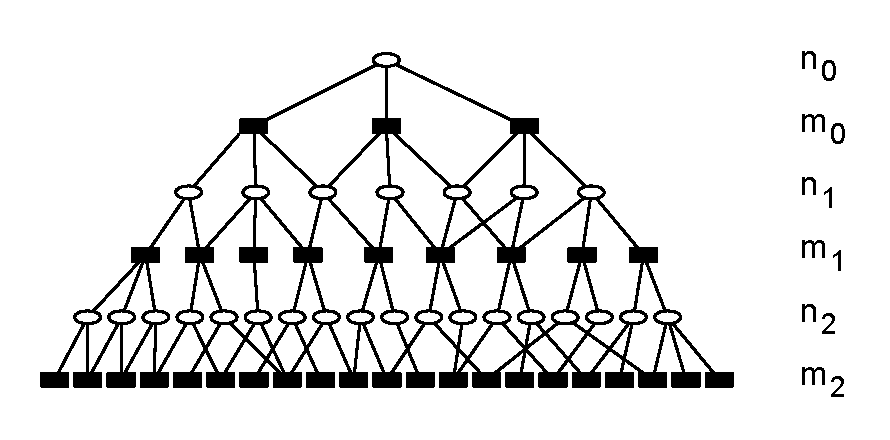
\includegraphics[width=5in]{figures/snowball_sample.eps}
\caption{Schematic of the Snowball Sampling Method}
% JMH to DJW: can we change levels to u_0, l_0, u_1, l_0, etc? (for users @ level 0, lists @ level 0, ...)
\label{fig:snowball_sample_schematic}
\end{figure}

Table~\ref{tab:snowball_sample} shows how many (a) users and (b) lists were
obtained at each level of the snowball sample.  In total, $495,000$ users
were obtained, who appeared on $7,000,000$ lists.  Because users can be
listed in multiple categories (e.g., Oprah Winfrey is frequently included
in lists of ``celebrity'' and ``media''), we next compute a user $u$'s
membership score in category $c$:
\begin{equation}
w_{uc}=\frac{n_{uc}}{N_c},
\end{equation}
where $n_{uc}$ is the number of lists in category $c$ that contain user $u$
and $N_c$ is the total number of lists in category $c$. We then assign each
user to the category in which he or she has the highest membership
score. Users that appear in the follower graph but not in the snowball
sample are assigned to the ``ordinary'' category.


\begin{table}
\centering
%\begin{scriptsize}
\caption{Snowball Sample}
\label{tab:snowball_sample}
\begin{tabular}{|c|r|r|r|r|}
\hline
Level 		& celeb	& media & org 	& blog \\ \hline
$u_0$		& 3 	& 2 	& 4		& 32 \\ \hline
$l_0$		& 2342 	& 11403	& 1170 	& 1347 \\ \hline \hline
$u_1$		& 3607 	& 5025 	& 20122	& 16317 \\ \hline
$l_1$		& 30490 & 71605	& 4970 	& 9546 \\ \hline \hline
$u_2$		& 108836 & 309056 & 115034 & 140251 \\ \hline
$l_2$		& 91873 & 171912 & 22518 & 19946 \\ \hline
\end{tabular}
%\end{scriptsize}
\end{table}


\subsection{Activity Sample of Twitter Lists}
Although the snowball sampling method is convenient and is easily
interpretable with respect to our theoretical motivation, it is also
potentially biased by our particular choice of seeds. To address this
concern, we also generate a sample of users based on their
activity. Specifically, we crawl all lists associated with all users who
tweet at least once every week for the entire observation period.
% DW to SW: Do we retain users who tweet at least once per week, or who
% tweet at least one URL per week?  
% SW: the first case: tweet at least once per week.

This ``activity-based'' sampling method, which yields $750,000$ users and
$5,000,000$ lists (see Table~\ref{tab:sampling-comp} for comparison to the
snowball method), is also clearly biased towards users who are consistently
active. Importantly, however, the bias is likely to be quite different from
any introduced by the snowball sample; thus obtaining similar results from
the two samples should give us confidence that our findings are not
artifacts of the sampling procedure.

\begin{table}
\centering
%\begin{scriptsize}
\begin{tabular}{|c|r|r|r|r|} \hline
 & \multicolumn{2}{|c|} {Snowball Sample} & \multicolumn{2}{|c|} {Activity Sample} \\ \hline
\textit{category} & \# of users & \# of lists & \# of users  & \# of lists\\ \hline
celeb & 108,836 & 91,873 & 22,803 & 68,810 \\ \hline
media & 309,056 & 171,912 & 66,300 & 145,176\\ \hline
org & 115,034 & 22,518 & 19,726 & 16,532\\ \hline
blog & 140,251& 19,946 & 49,987 &17,259\\
\hline
\end{tabular}
\caption{Statistics of crawled lists. The number of users refers only to
  people who appear in at least one list of the specific category.}
\label{tab:sampling-comp}
%\end{scriptsize}
\end{table}

% \begin{figure}
% \centering
% 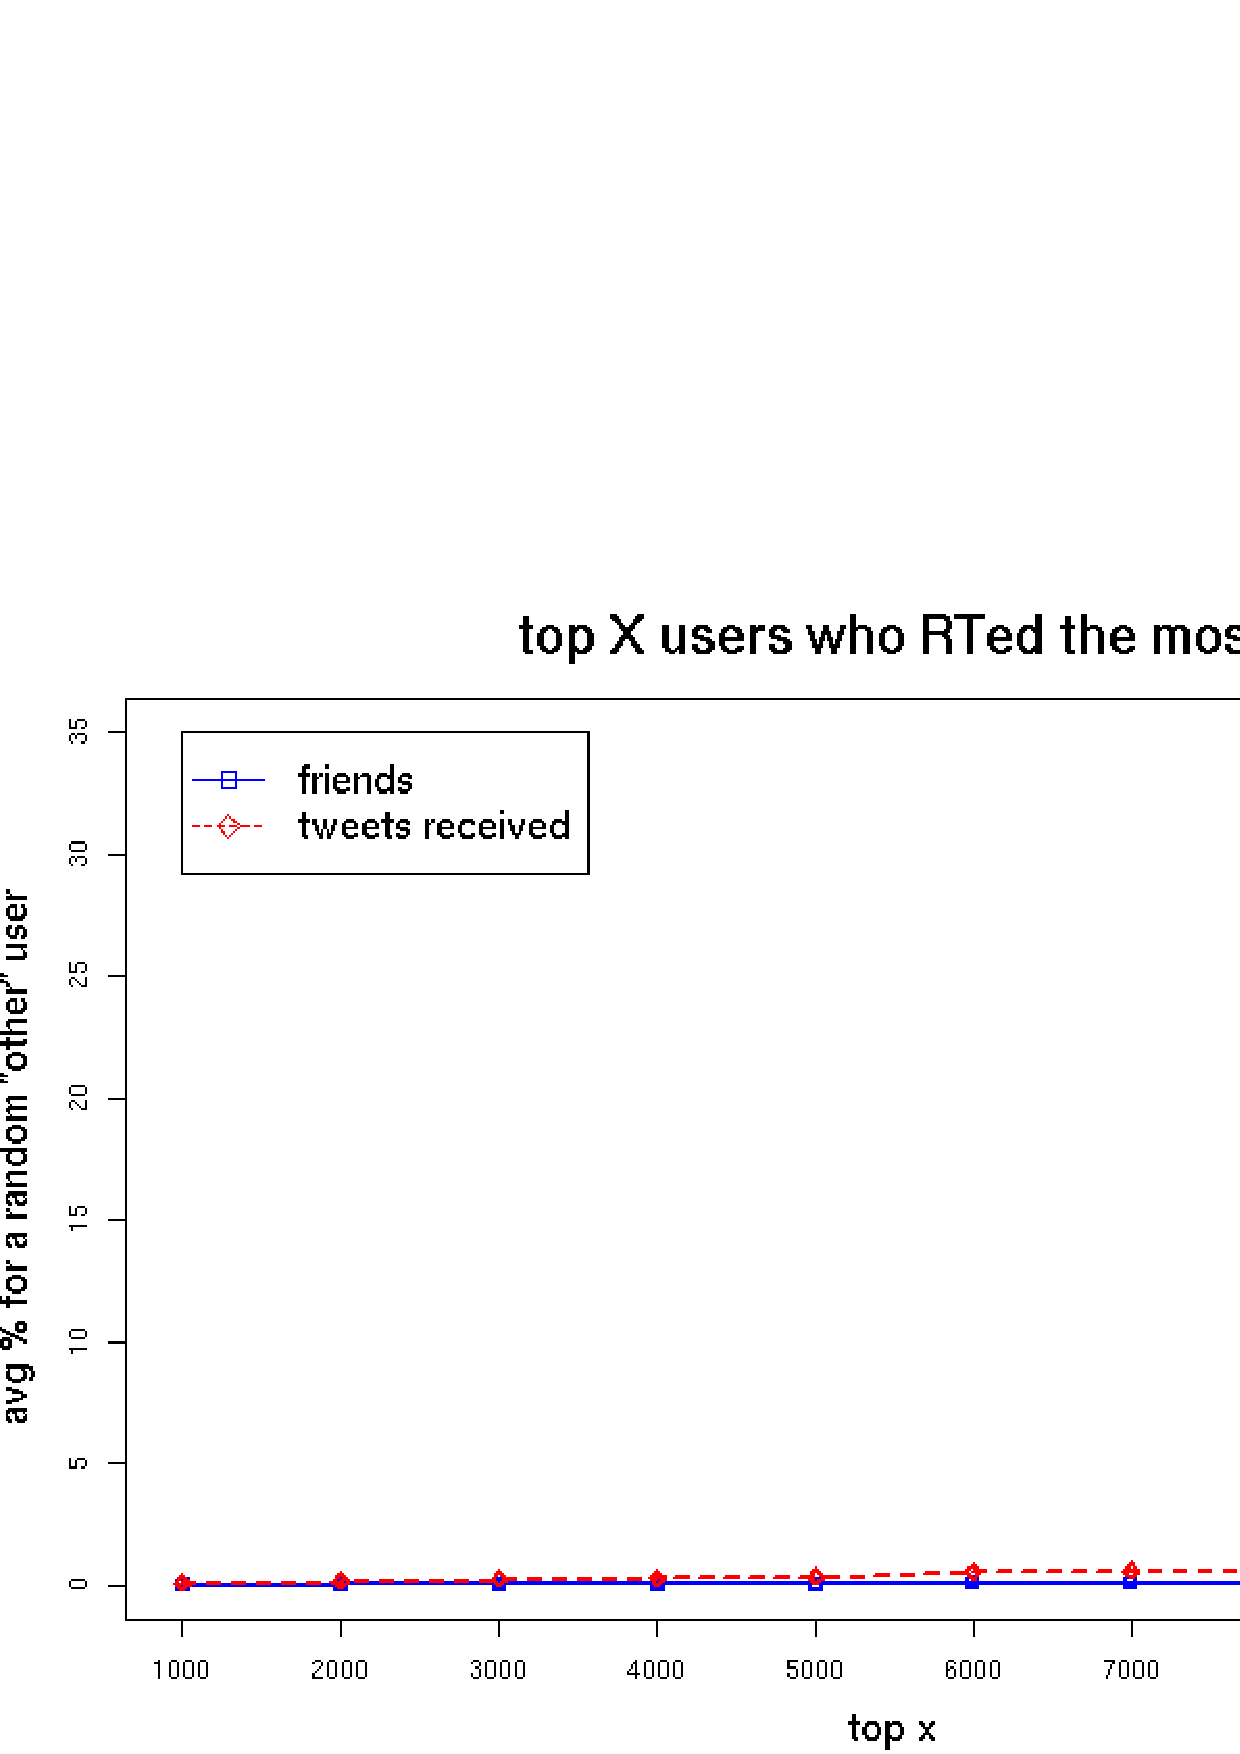
\includegraphics[width=3in]{figures/mostRTing_user_outflow_to_random_other_users.png}
% \caption{}
% \label{top_k_volume_other}
% \end{figure}

\section{Distribution of attention}

After categorizing people into categories, we can calculate the amount of attention sent and received by each category, at a global level. The approach we take is to measure the reach of the ``elite'' categories, which can be considered as the influence of each category, as well as an estimate of the impact of the information introduced by each category. In other words, it is the maximal reach of the information produced by each category.


\subsection{Concentration of attention}
\label{sec:attention}
With either sampling method, the initial categorization of users is quite
coarse and noisy as a result of the arbitrary labeling allowed in Twitter
Lists.  To filter categories to the most representative users, we further
rank the users in each of the 4 elite categories by how frequently they are
listed in each category, and take only the top $k$ users in each category,
relabeling the remainder as ``ordinary'' users. To determine the
appropriate $k$, we measure the flow of information from the four elite
categories to an average ``ordinary'' user in two ways: the proportion of
people the user follows in each category, and the proportion of tweets the
user received from everyone the user follows in each category.  We sampled
100K random ``ordinary'' users and calculated the average information flow
from the ``elite'' users using these two measures.

Figure~\ref{fig:attention_elites_snowball} shows that each category
accounts for a significant share of both the following links and also the
tweets received by an average user, where celebrities outrank all other
categories, followed by the media, organizations, and bloggers.  Also of
note is that the bulk of the attention is accounted for by a relatively
small number of users within each category, as evidenced by the relatively
flat slope of the attention curves in Figure
\ref{fig:attention_elites_snowball}. In order to define which users should
be classified as ``elites'', we seek a tradeoff between (a) keeping each
category relatively small, so as not to include users who are not
distinguishable from ordinary users, while (b) maximizing the volume of
attention that is accounted for by each category. In addition, it is also
desirable to make the four categories the same size, so as to facilitate
comparisons.  Balancing these requirements, we therefore choose 5K as a
cut-off for the elite categories.

\begin{figure}[ht]
\centering
\subfigure[Snowball sample]{
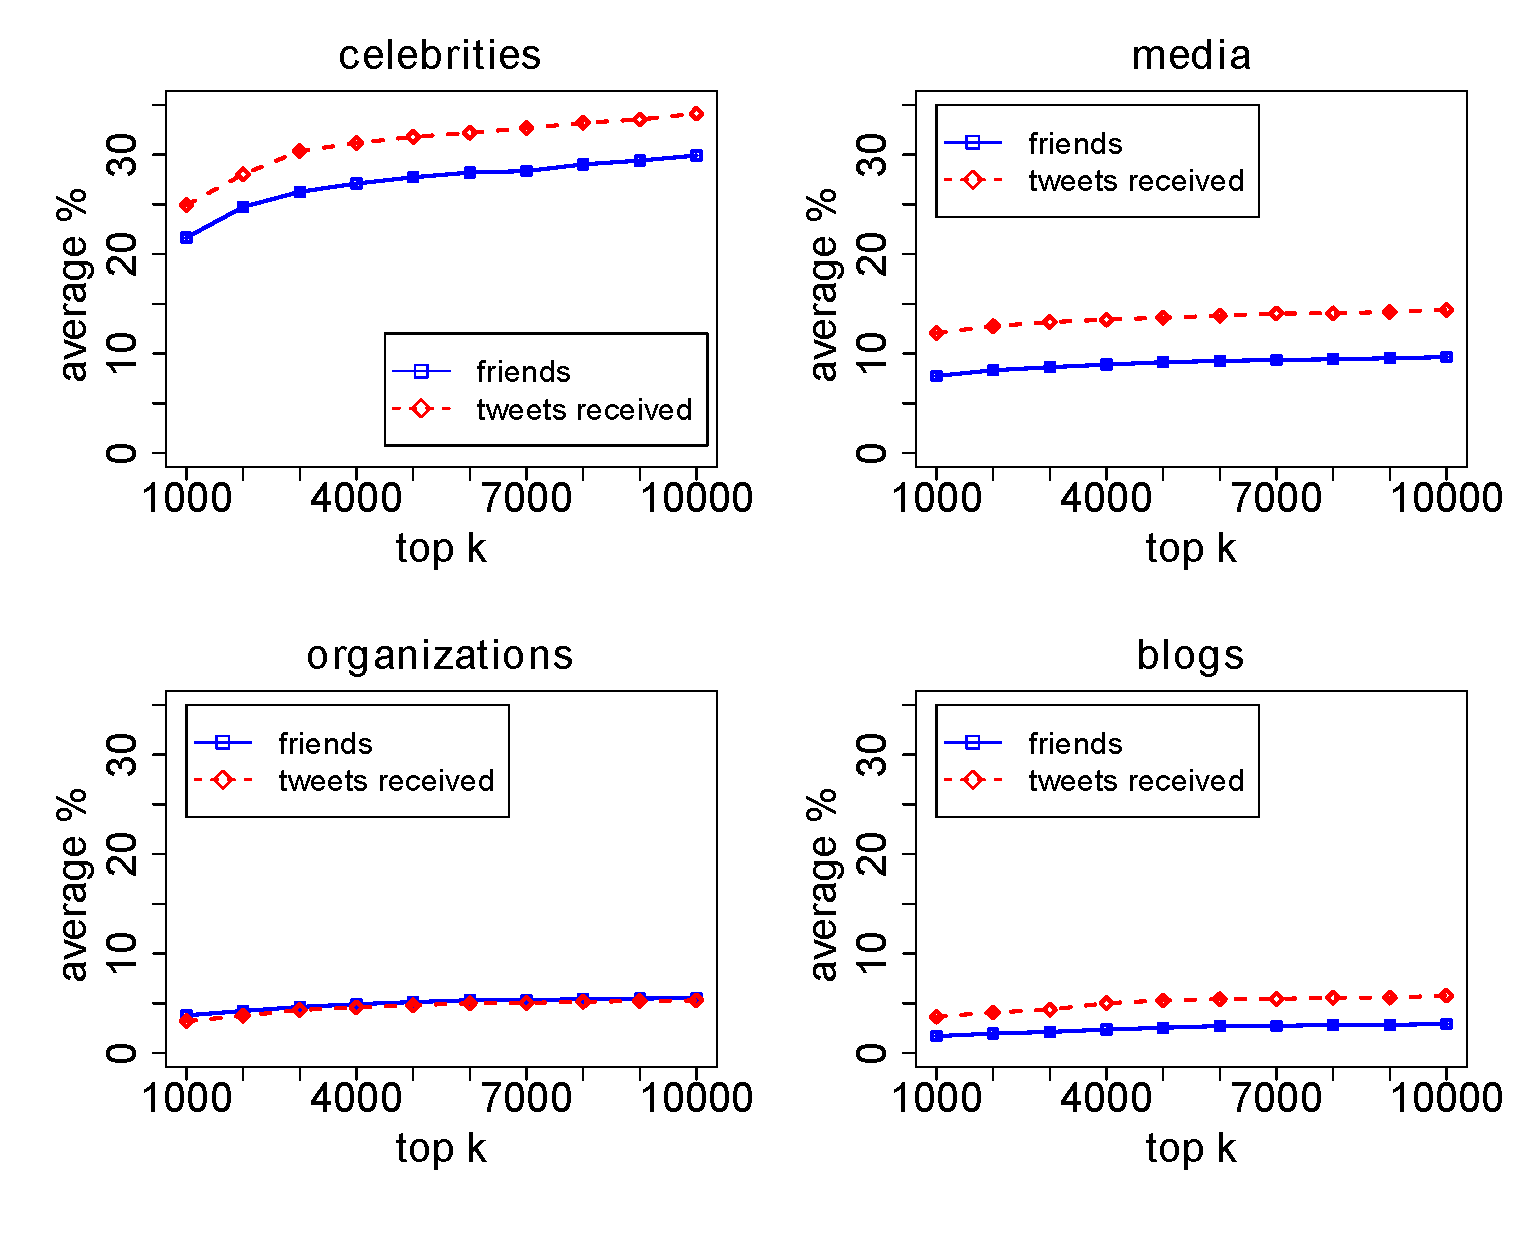
\includegraphics[width=5in]{figures/top_users_outflow_to_random_other_users_500K.eps}
\label{fig:attention_elites_snowball}
}
\subfigure[Activity sample]{
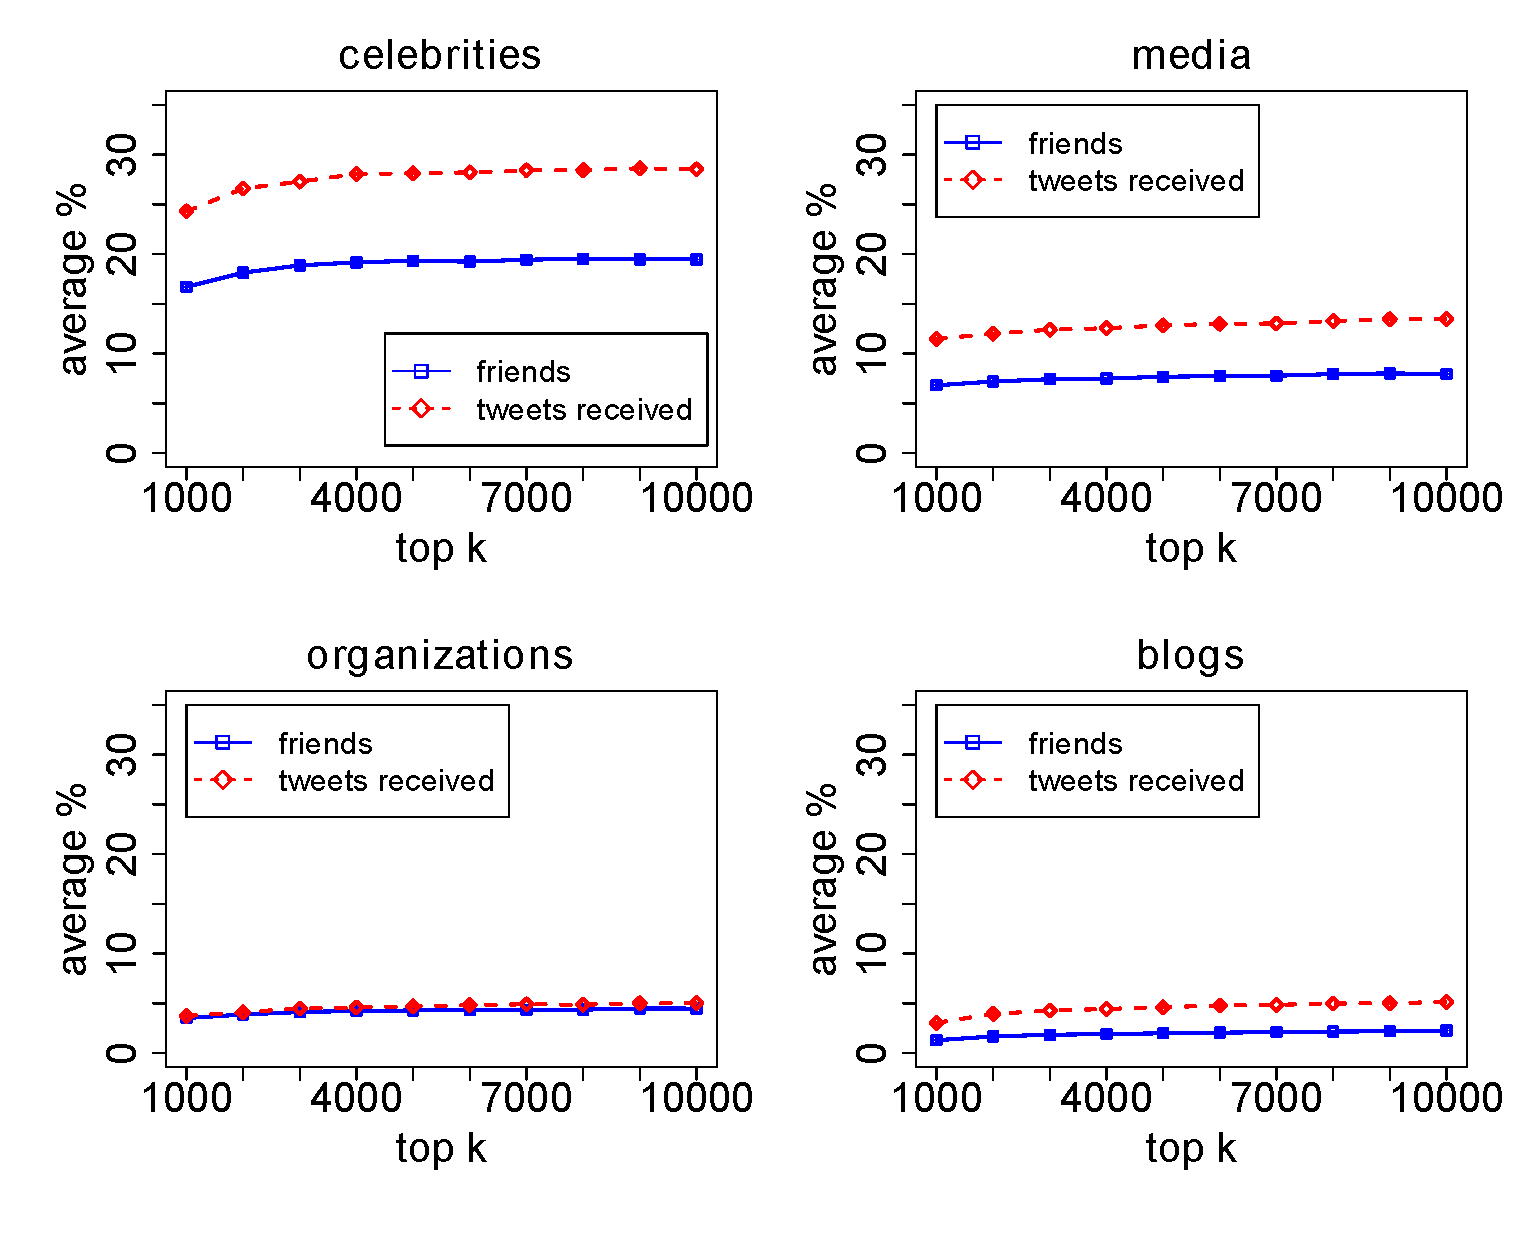
\includegraphics[width=5in]{figures/top_users_outflow_to_random_other_users_800K.eps}
\label{fig:top_k_elite_volume}
}
\caption{Average fraction of $\#$ following (blue line) and $\#$
  tweets (red line) for a random user that are accounted for by the
  top K elites users crawled}
\label{fig:attention_to_top_k_elite}
\end{figure}

%\begin{figure}
%\centering
%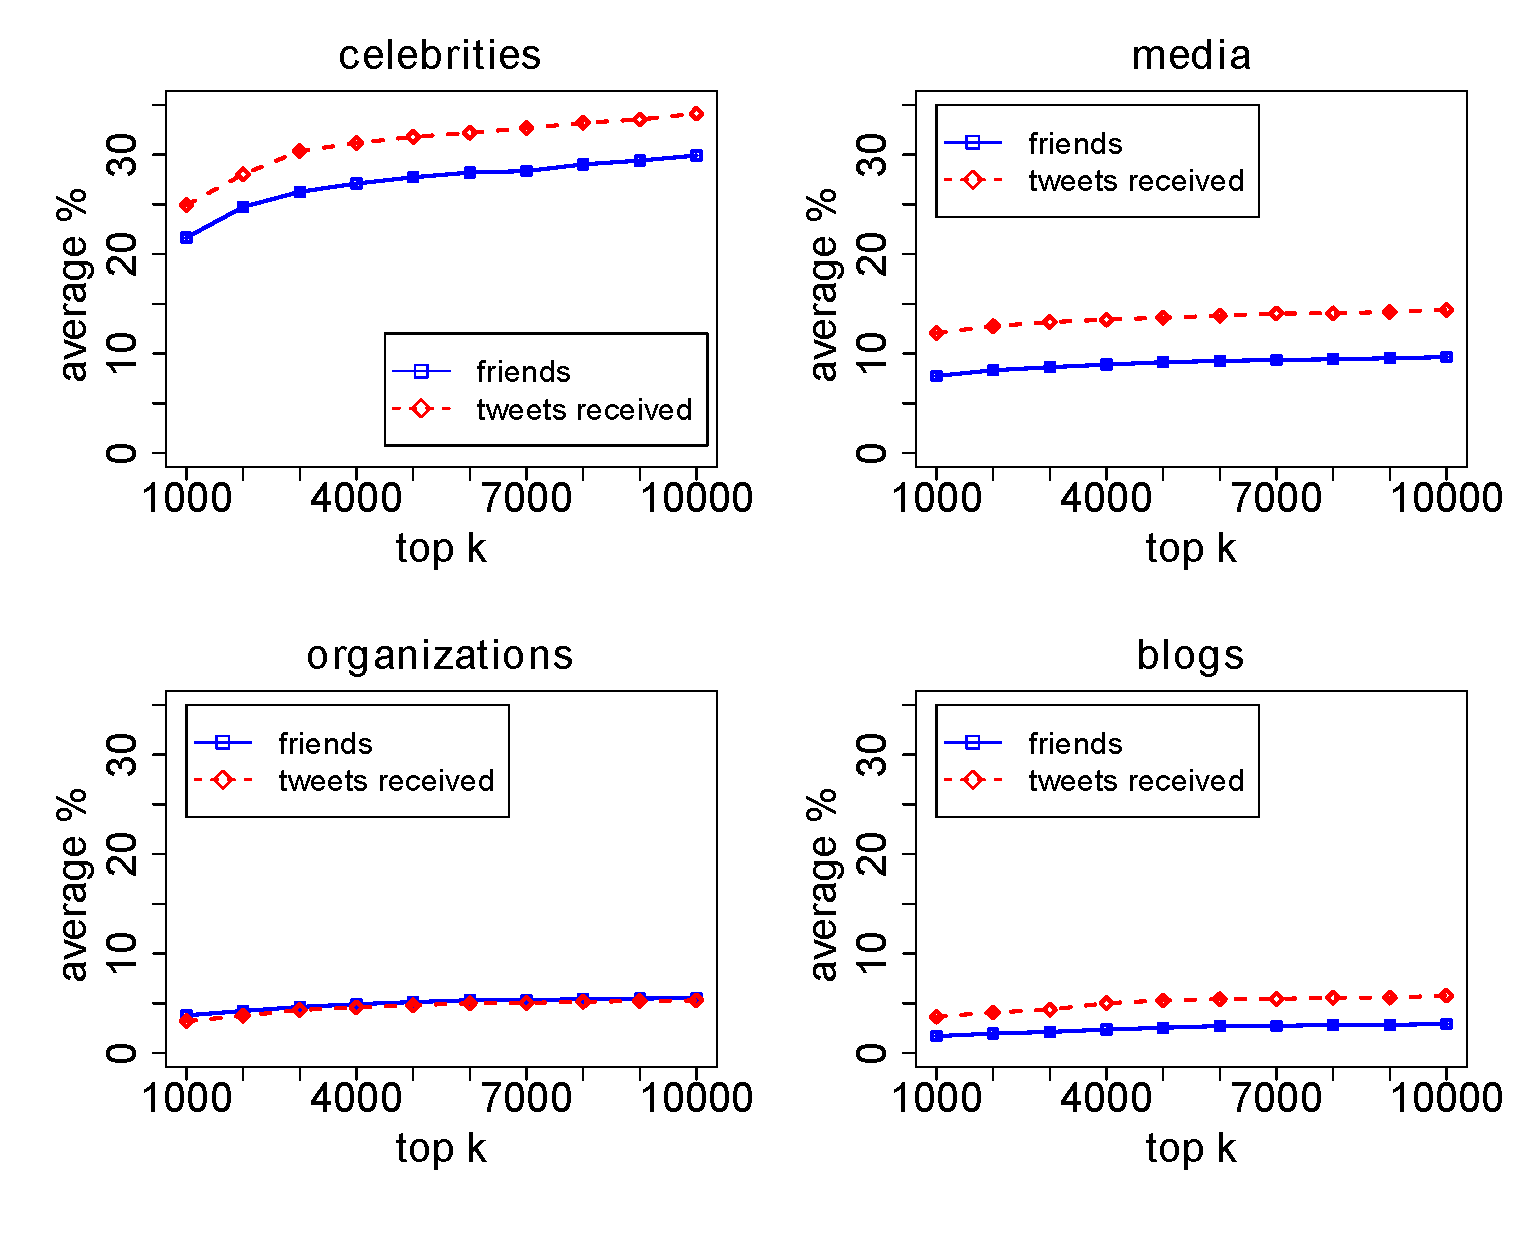
\includegraphics[width=3in]{figures/top_users_outflow_to_random_other_users_500K.eps}
%\caption{Average fraction of $\#$ following (blue line) and $\#$
%  tweets (red line) for a random user that are accounted for by the
%  top K elites users crawled}
%\label{fig:attention_elites_snowball}
%\end{figure}

%\begin{figure}
%\centering
%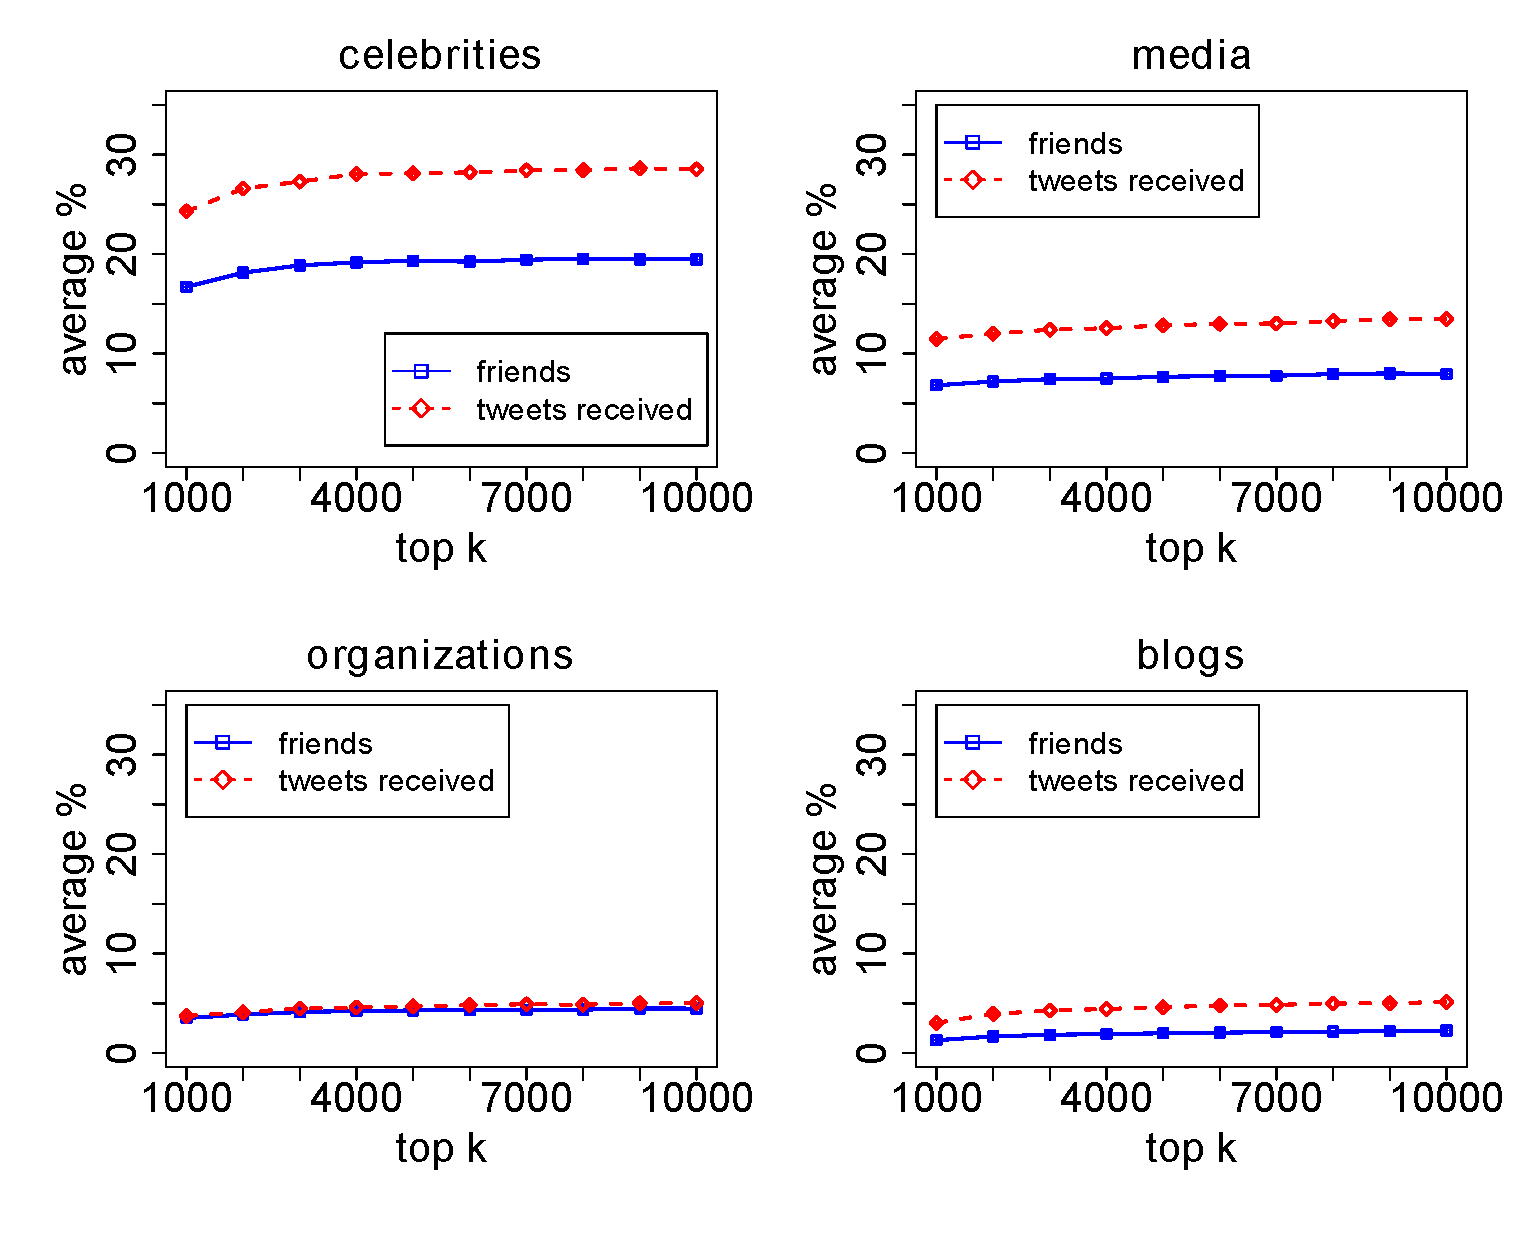
\includegraphics[width=3in]{figures/top_users_outflow_to_random_other_users_800K.eps}
%\caption{Average fraction of $\#$ following (blue line) and $\#$ tweets
%  (red line) for a random user that are accounted for by the top $k$ users
%  classified in one of our four categories}
%\label{fig:top_k_elite_volume}
%\end{figure}


Consistent with this view, we find that the population of users identified
by the activity sample is somewhat different from the snowball sample: the
intersection of the two populations is only 20$\%$ (100,000
accounts). However, the intersection of the top $k$ users in each
population increases as $k$ decreases: for the top $5,000$ users in each
category, the intersection is $41\%$, and for the top $1,000$ users it is
$51\%$. Thus, although the population of consistently active users is
somewhat different from those reached with the snowball sample, the most
frequently listed users in both populations tend to be similar. In
addition, Figure \ref{fig:top_k_elite_volume} shows that the attention paid
to the top $k$ users in the four categories is essentially the same as for
the snowball sample.  Thus in the rest of this paper, when we talk about
``celebrity'', ``media'', ``organization'', ``blog'', we mean the top 5K
users listed as ``celebrity'', ``media'', ``organization'', ``blog'',
respectively, drawn from the snowball sample. Table
\ref{tab:top_k_examples} shows the top 5 users in each of
the four categories.

%  while Figure \ref{top_k_other_volume} reassures us
% that again the unclassified users account for at most a negligible
% fraction of attention.

% JMH to SW: should the axis be adjusted here for better resolution? or
% will this give the false appearance that there's lots of variation wrt x?
% SW: which axis? 

\begin{table}
\centering
%\begin{scriptsize}
\caption{Top 5 users in each category}
\label{tab:top_k_examples}
\vspace{2pt}
\begin{tabular}{|c|c|c|c|} 
\hline 
%\multicolumn{4}{|c|} {Top 5 users} \\ 
%\hline
\textit{Celebrity} & \textit{Media} & \textit{Org} & \textit{Blog} \\ 
\hline
aplusk & cnnbrk & google & mashable \\
ladygaga & nytimes & Starbucks & problogger \\
TheEllenShow & asahi & twitter & kibeloco \\
taylorswift13 & BreakingNews & joinred & naosalvo \\
Oprah & TIME & ollehkt & dooce \\
\hline 
%\multicolumn{4}{|c|} {Bottom 5 users} \\ 
%\hline
%\textit{Celebrity} & \textit{Media} & \textit{Org} & \textit{Blog} \\ 
%\hline
%rajolaurel & singaporenews & worldvisioncan & nicolamattine \\
%wongfupro & TelegraphSci & fujiqnow & machedavvero \\
%FUCKCITY & SZ\_Wirtschaft & KNT\_gakusei & BrideTide \\
%tonyfernandes & TheOaklandPress & overdrive\_jp & theselvedgeyard \\
%Silver90210 & USDOL & ProOkubo & averyps \\
%\hline
\end{tabular}
%\end{scriptsize}
\end{table}


To confirm the validity of these categories, we now consider the number of
URLs introduced by various categories. As Table \ref{tab:urls_initiated}
(left column) shows, the vast majority of URLs are initiated by ordinary
users, not by any of the elite categories.  This result, however, is
deceptive: as we have just determined, our elite categories number only
$20K$ users in total, whereas we classify over $40M$ users in the
``ordinary'' category.  A more calibrated view is presented in the right
hand column of Table \ref{tab:urls_initiated}, which shows the per-capita
number of URLs originating from various categories.  Here it is clear that
users classified as ``media'' far outproduce all other categories, followed
by bloggers, organizations, and celebrities. In contrast to the previous
result, ordinary users originate on average only about $6$ URLs
each---far fewer than any category of elite users.

%%DW: Need to note at some point in this section that from now on we will
%%use snowball sample; all results are the same.
%%WM: done, in previous paragraph

% JMH: Need to add a second column for per-capita initiations.
% WM: done
\begin{table}
\centering
\caption{\# of URLs initiated by category}
\label{tab:urls_initiated}
\begin{tabular}{l r r}
\textit{category} & \# of URLs & per-capita \# of URLs \\ 
\hline
celeb	& 139,058 & 27.81 \\ 
media	& 5,119,739 & 1023.94 \\ 
org	& 523,698 & 104.74 \\ 
blog	& 1,360,131 & 272.03 \\ 
other	& 244,228,364 & 6.10\\
\end{tabular}
\end{table}


Conceivably, our classification scheme above has omitted an important
category; that is, within the current ``other'' category may be hidden
additional categories of opinions.  As Figure~\ref{fig:top_k_volume_other}
shows, however, even the top 10,000 most followed of these users
accounts for a negligible fraction of attention among the remaining
population.  
 
\begin{figure}
\centering
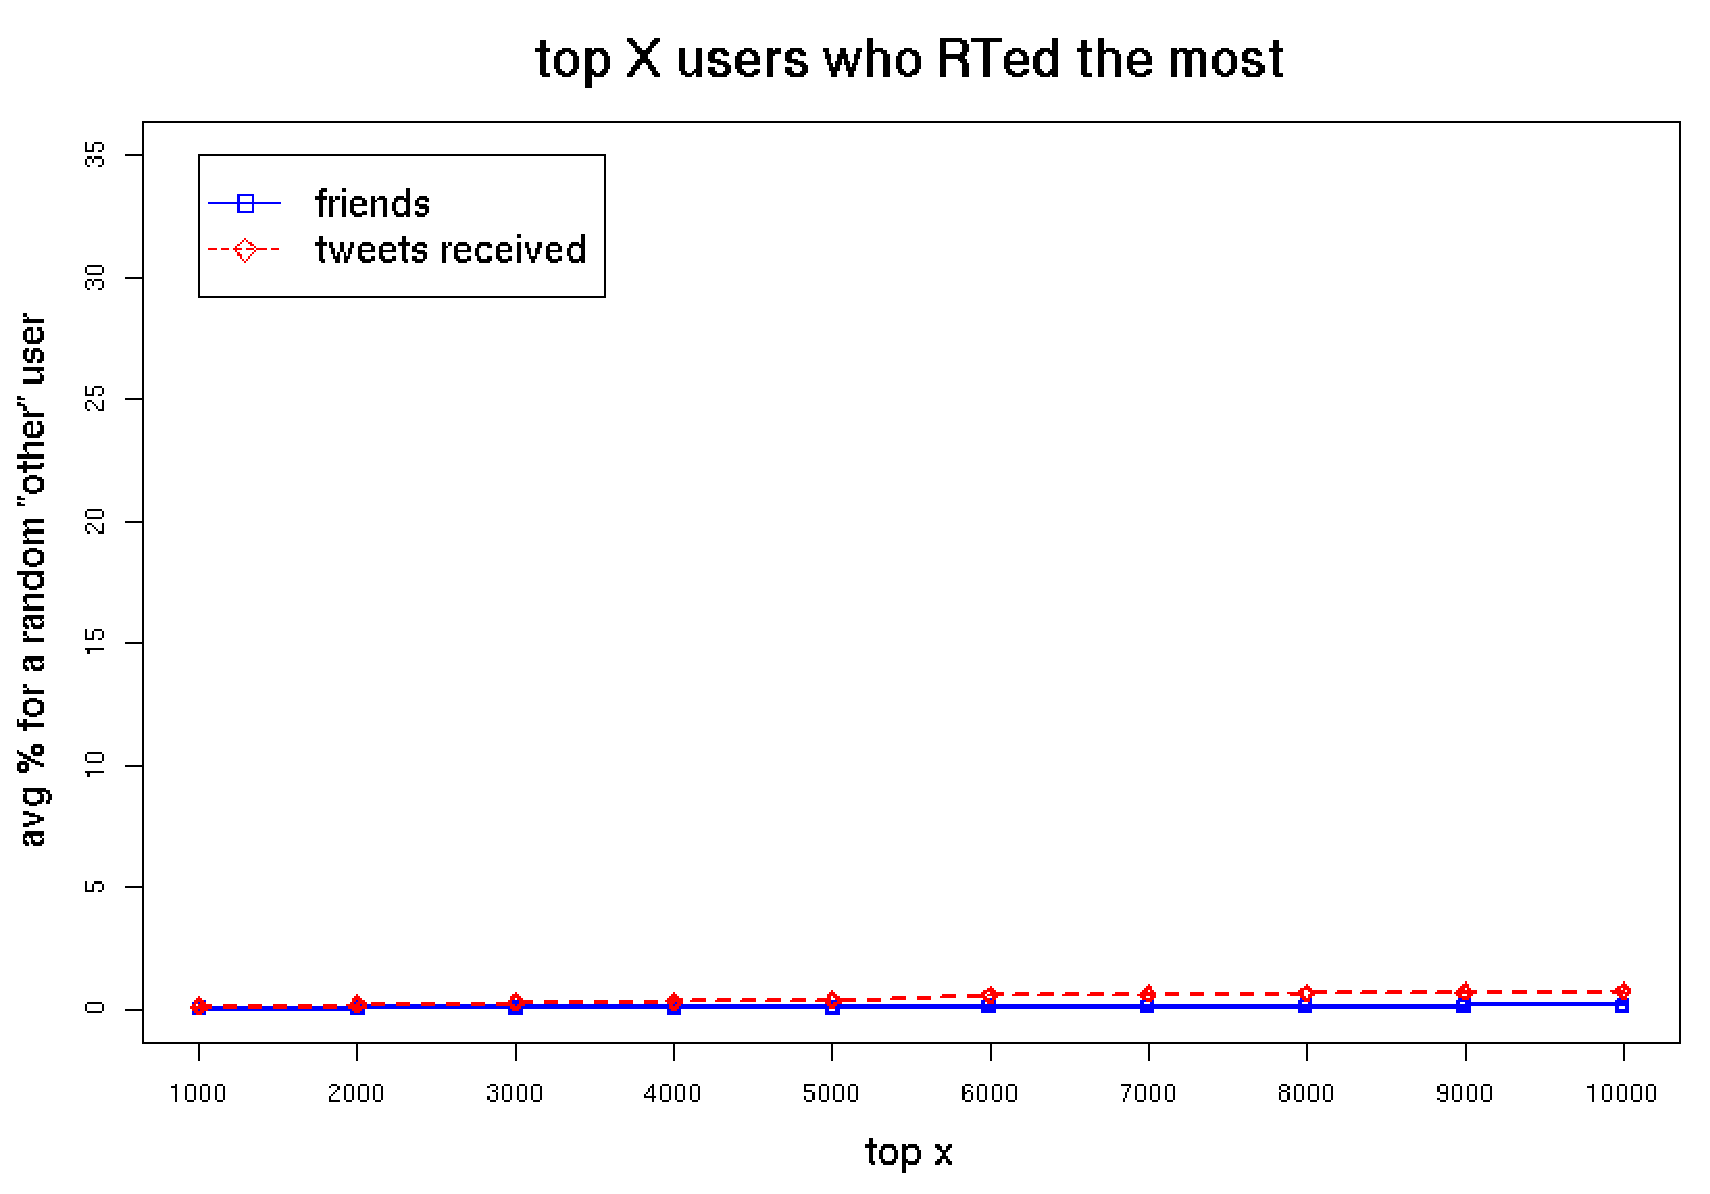
\includegraphics[width=5in]{figures/mostRTing_user_outflow_to_random_other_users.eps}
\caption{Average fraction of $\#$ following (blue line) and $\#$
  tweets (red line) for a random user that are accounted for by the
  top K most retweeted users in the ``Other'' category}
\label{fig:top_k_volume_other}
\end{figure}


\subsection{Homophily of influence}

As indicated above, the top $20K$ elite users account for almost $50 \%$ of
all attention within Twitter; yet this population of users comprises less
than $0.05\%$ of the population.
% As we can see in Figure \ref{fig:topuser_to_other}, for an ordinary
% Twitter user, a significant portion of people he follows are among the
% small number of ``elite'' users we identified, and an even higher
% portion of the tweets he receives are directly from those elite users.
In other words, although Twitter clearly reflects the conventional wisdom
that audiences have become increasingly fragmented, it nevertheless shows
remarkable concentration of information production and received attention
among a relatively small number of actors. Even if the media has lost
attention relative to other elites, information flows have not become
egalitarian by any means.

The prominence of elite users raises the question of how these different
categories listen to each other.  To address this issue, we compute the
percentage of following links and received tweets among elite
categories. Specifically, Table \ref{tab:flow_among_categories} shows the
average percentage of friends/tweets category $i$ get from category
$j$. Table \ref{tab:flow_among_categories} shows striking homophily with
respect to attention: celebrities overwhelmingly pay attention to other
celebrities, media actors pay attention to other media actors, and so on.
The one slight exception to this rule is that organizations pay more attention
to bloggers than to themselves.  In general, in fact,
attention paid by organizations is more evenly distributed across
categories than for any other category.

\begin{table}
\centering
%\begin{scriptsize}
\caption{Information flow among the elite categories}
\label{tab:flow_among_categories}
\vspace{2pt}
\begin{tabular}{|c|r|r|r|r|}
\hline
\% of friends &	in celeb  &	in media &	in org	& in blog \\\hline
celeb	& \bf{30.56} & 3.63 & 1.99 & 1.64 \\ \hline
media	& 3.59 & \bf{16.67} & 2.07 & 2.15 \\ \hline
org	& 3.62 & 3.33 &	\bf{7.38} & 2.65 \\ \hline
blog	& 4.41 & 2.27 &	2.03 &	\bf{10.25} \\ \hline
\hline
\% of tweets &	from celeb	&from media	&from org	&from blog \\ \hline
celeb	& \bf{38.27} & 6.23 & 1.55 & 3.98\\ \hline
media	&3.91 & \bf{26.22} & 1.66 & 5.69 \\ \hline
org	&4.64 & 6.41 &	8.05 & \bf{8.70} \\ \hline
blog	&4.94 & 3.89 & 1.58 & \bf{22.55} \\ \hline
\end{tabular}
%\end{scriptsize}
\end{table}

\begin{figure}
\centering
\includegraphics[width=5in]{figures/visualization_500K_tweets.eps}
\caption{Share of attention among elite categories}
\label{fig:topuser_to_other}
\end{figure}


\begin{comment}
\chapter{ZZZZZ: Transmissive probability}
ZZZZZ: should we combine this section with previous or next section?

For information that do spread, most previous works study the factors that contribute to the spread at each hop, independently. (ZZZZZ related work).

The categorization of actors, as introduced previously, also helped shed some light on the one-hop diffusion probability, depending on the type of users in the diffusion edge, and people's interest at different types of content.

My contribution:
\begin{enumerate}
\item Show homophily at diffusion;
\item Show difference in attention and influence (as measured by RTs)
\item Show people's interest at different content.
\end{enumerate}

\section{People}
The origin of information will influence how it will be RTed. 
\end{comment}

Figure~\ref{fig:attention_to_top_k_elite}, it should be noted, shows only how many URLs
are received by category $i$ from category $j$, a particularly
weak measure of attention for the simple reason that many
tweets go unread. A stronger measure of attention, therefore,
is to consider instead only those URLs introduced by
category $i$ that are subsequently retweeted by category $j$.
 
Before proceeding, it is helpful to differentiate between two mechanisms by
which information can diffuse in Twitter. The first is via retweeting, when
a user, having received a tweet, subsequently rebroadcasts it to his or her
own followers. In some instances, users retweet each other using the
official retweet function provided by Twitter, but in other cases they
credit the retweet with an informal convention, most commonly either ``RT
@user" or ``via @user.'' The second mechanism is what we label
reintroduction, where a user independently tweets a URL that has previously
been introduced by another user.
%\footnote{Because users do sometimes retweet other users without
%  acknowledgement, we have likely misclassified some fraction of retweets
%  as reintroductions. One way to address this issue would be to count as a
%  retweet any appearance of a URL that had previously been tweeted by a
%  user that the current user is following. However, this solution raises
%  additional problems, and in any case does not occur sufficiently
%  frequently to affect our results; thus we treat all reappearances of a
%  URL as reintroductions unless specifically acknowledged as a retweet.}.

In addition to attention, Table \ref{tab:rt_breakdown} shows how much
information originating from each category is retweeted by other
categories, while Table \ref{tab:reintro_breakdown} shows how much is
subsequently reintroduced.  As with attention, both retweeting and
reintroduction activities are strongly homophilous among elite categories;
however, bloggers are disproportionately responsible for retweeting and
reintroducing URLs originated by all categories. This result reflects the
characterization of bloggers as recyclers and filters of information;
however, Table \ref{tab:rt_breakdown} and \ref{tab:reintro_breakdown} also
show that the total number of URLs either RT'd or reintroduced by bloggers
is vastly outweighed by the number retweeted or reintroduced by ordinary
users.  Even though on a per-capita basis, therefore, bloggers
disproportionately occupy the role of information recyclers, their actual
impact is relatively minimal (see Figure \ref{fig:topuser_to_other}).

\begin{table*}
\centering
\caption{RTs among categories}
\label{tab:rt_breakdown}
\begin{tabular}{|l|r|r|r|r|r|r|}
\hline
 &  by celeb & by media & by org & by blog & by other & TOTAL\\ \hline
celeb & 4,334 & 1,489 &	1,543 &	5,039 &	1,070,318  & 1,082,723\\ \hline
media & 4,624 & 40,263 & 7,628&32,027 & 5,204,719  & 5,289,261\\ \hline
org & 1,570 & 2,539 & 18,937 & 11,175 & 1,479,017 & 1,513,238\\ \hline
blog & 3,710 & 6,382 & 5,762 & 99,818 & 3,457,631 & 3,573,303\\ \hline
other & 34,455 & 93,934 & 86,630 & 318,537 & 34,814,456 & 35,348,012\\ \hline
\end{tabular}
\end{table*}

\begin{table*}
\centering
\caption{Re-introductions among categories}
\label{tab:reintro_breakdown}
\begin{tabular}{|l|r|r|r|r|r|r|}
\hline
& by celeb & by media & by org & by blog & by other & TOTAL\\ \hline
celeb &	2,868 & 1,239 & 522 & 1,664 & 488,229 & 494,522\\ \hline
media & 1,678 & 205,165 & 2,439	& 9,681	& 2,006,888 & 2,225,851\\ \hline
org & 816 & 1,511 & 8,628 & 3,711 & 610,373 & 625,039\\ \hline
blog & 1,415	& 5,644	& 1,416	& 52,909 & 1,148,137 & 1,209,521\\ \hline
other & 45,547 & 793,741 & 69,441 & 335,690 & 86,853,224 & 88,097,643\\ \hline
\end{tabular}
\end{table*}

\begin{figure}
\centering
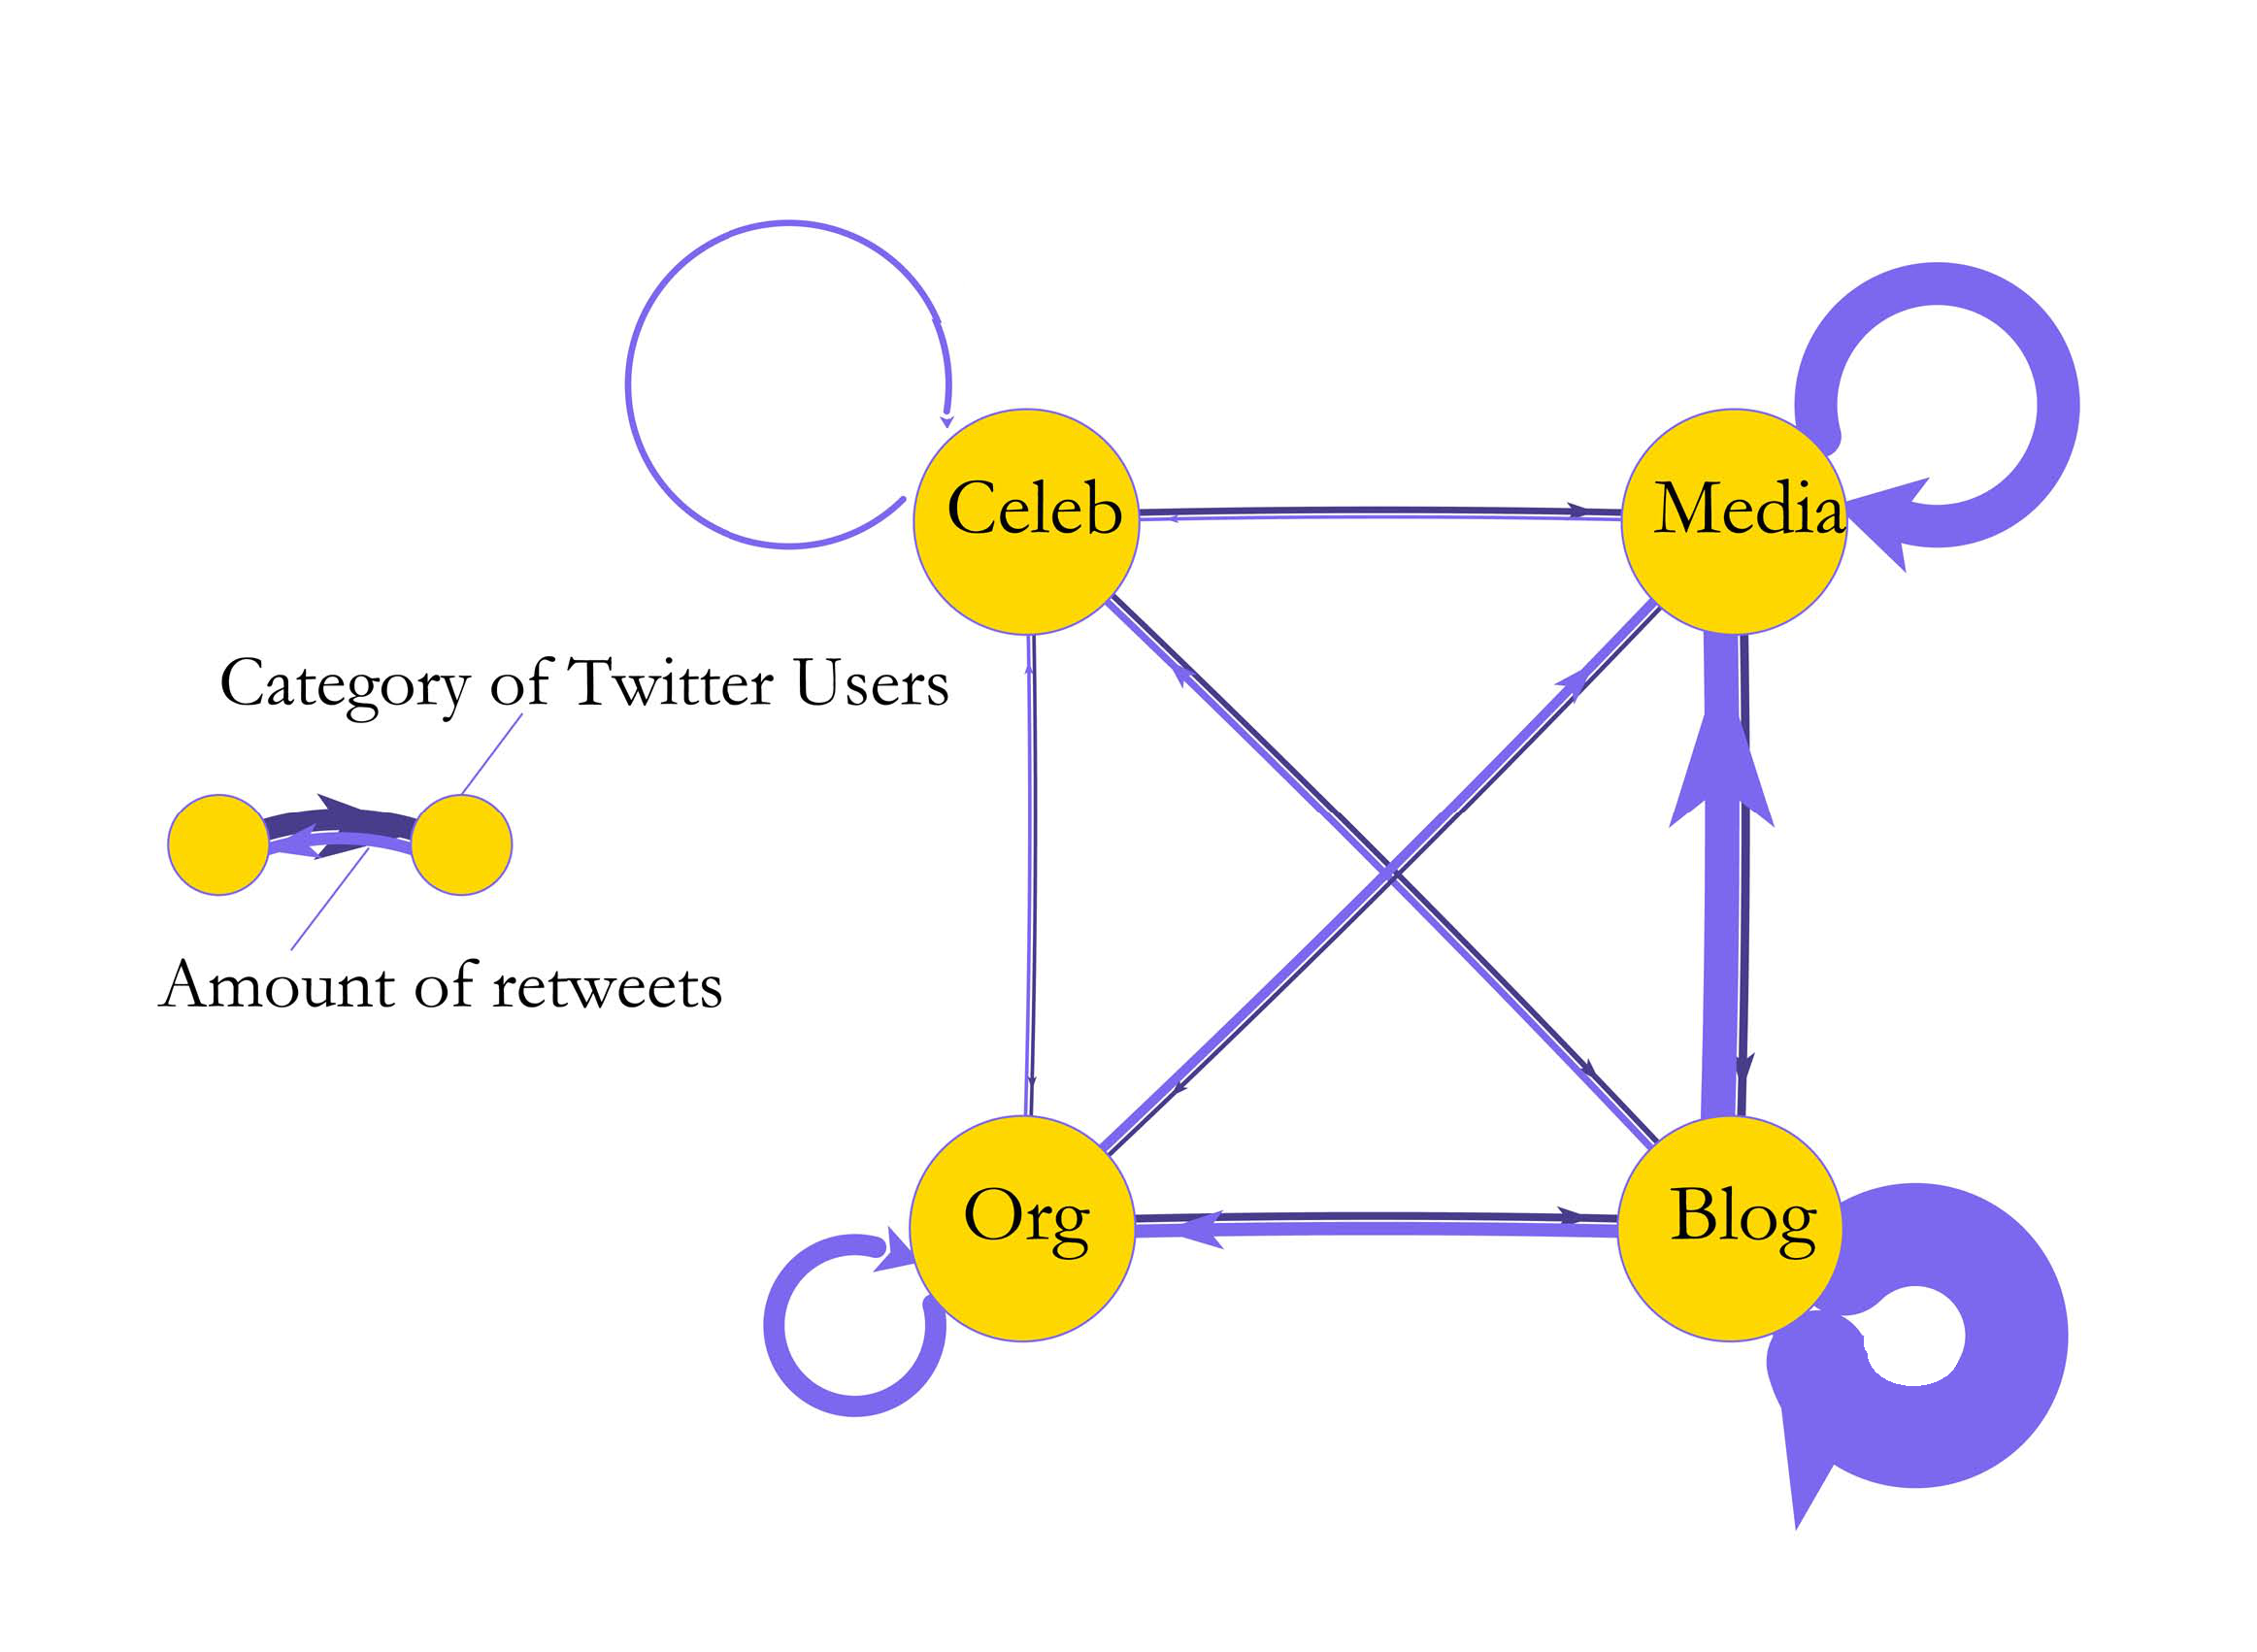
\includegraphics[width=5in]{figures/rt_topUsers_500K.eps}
\caption{RT behavior among elite categories}
\label{fig:RT_topuser}
\end{figure}


\section{Revisiting two-step flow theory: what are the opinion leaders?}
\label{sec:two-step}
The two-step flow theory, first proposed in the 50's, is still one of the most successful theories that captured the dueling importance of mass media and interpersonal influence.  The essence of the two-step flow is that
information passes from the media to the masses not directly, as supposed
by early theories of mass communication, but rather via an intermediary
layer of \emph{opinion leaders}, who act as filters and interpreters for their
followers. Although deeply ackowledged by marketers, it has been difficult to identify opinion leaders at a large scale, or quantify their impact to the public. As we have already gathered a confident list of mass media accounts, it becomes a natural problem for us to verify the two-step flow theory on Twitter, and ask, what are the opinion leaders, and what proportion of the information originating from media sources is broadcast directly to the masses, and what proportion is transmitted indirectly via some population of intermediaries. In addition, we may inquire whether these intermediaries,
to the extent they exist, are drawn from other elite categories or from
ordinary users, as claimed by the two-step flow theory; and if the latter,
in what respects they differ from other ordinary users.

Before proceeding with this analysis, we note that there are two ways
information can pass through an intermediary in Twitter. The first is
via retweeting, which occurs when a users explicitly rebroadcasts a
URL that he or she has received from a friend, along with an explicit
acknowledgement of the source---either using the official retweet
functionality provided by Twitter or by making use of an informal
convention such as ``RT @user" or ``via @user.''  Alternatively, a
user may tweet a URL that has previously been posted, but without
acknowledgement of a source; in this case we assume the information
was independently rediscovered and label this a ``reintroduction'' of
content.
%The second mechanism is what we label reintroduction, where a user
%subsequently tweets a URL that has previously been introduced by another
%user, but without the acknowledgment, in which case we assume the
%information has been rediscovered independently.
% (where we note that because users do sometimes retweet other users
% without acknowledgement, we have likely misclassified some fraction of
% retweets as reintroductions).  
For the purposes of studying when a user receives information directly from
the media or indirectly through an intermediary, we treat retweets and
reintroductions equivalently.  If the first occurrence of a URL in Twitter
came from a media user, but a user received the URL from another source,
then that source can be considered an intermediary, whether they are
citing the source within Twitter by retweeting the URL, or reintroducing
it, having discovered the URL outside of Twitter.

To quantify the extent to which ordinary users get their information
indirectly versus directly from the media, we sampled 1M random ordinary
users\footnote{As before, performing this analysis for the entire
  population of over 40M ordinary users proved to be computationally
  unfeasible.}, and for each user, counted the number $n$ of bit.ly URLs
they had received that had originated from one of our 5K media users, where
of the 1M total, 600K had received at least one such URL.  For each member
of this 600K subset we then counted the number $n_2$ of these URLs that
they received via non-media friends; that is, via a two-step flow. The
average fraction $n_2/n = 0.46$
%%DW: Check that this number stays the same
therefore represents the proportion of media-originated content that
reaches the masses via an intermediary rather than directly. As Figure
\ref{fig:two_step_volume} shows, however, this average is somewhat
misleading.  In reality, the population comprises two types---those who
receive essentially all of their media-originating information via two-step
flows and those who receive virtually all of it directly from the media.
Unsurprisingly, the former type is exposed to less total media than the
latter.  What is surprising, however, is that even users who received up to
100 media URLs during our observation period received all of them via intermediaries.


%%DW to SW: need to put figure in SVN
\begin{figure}
\centering
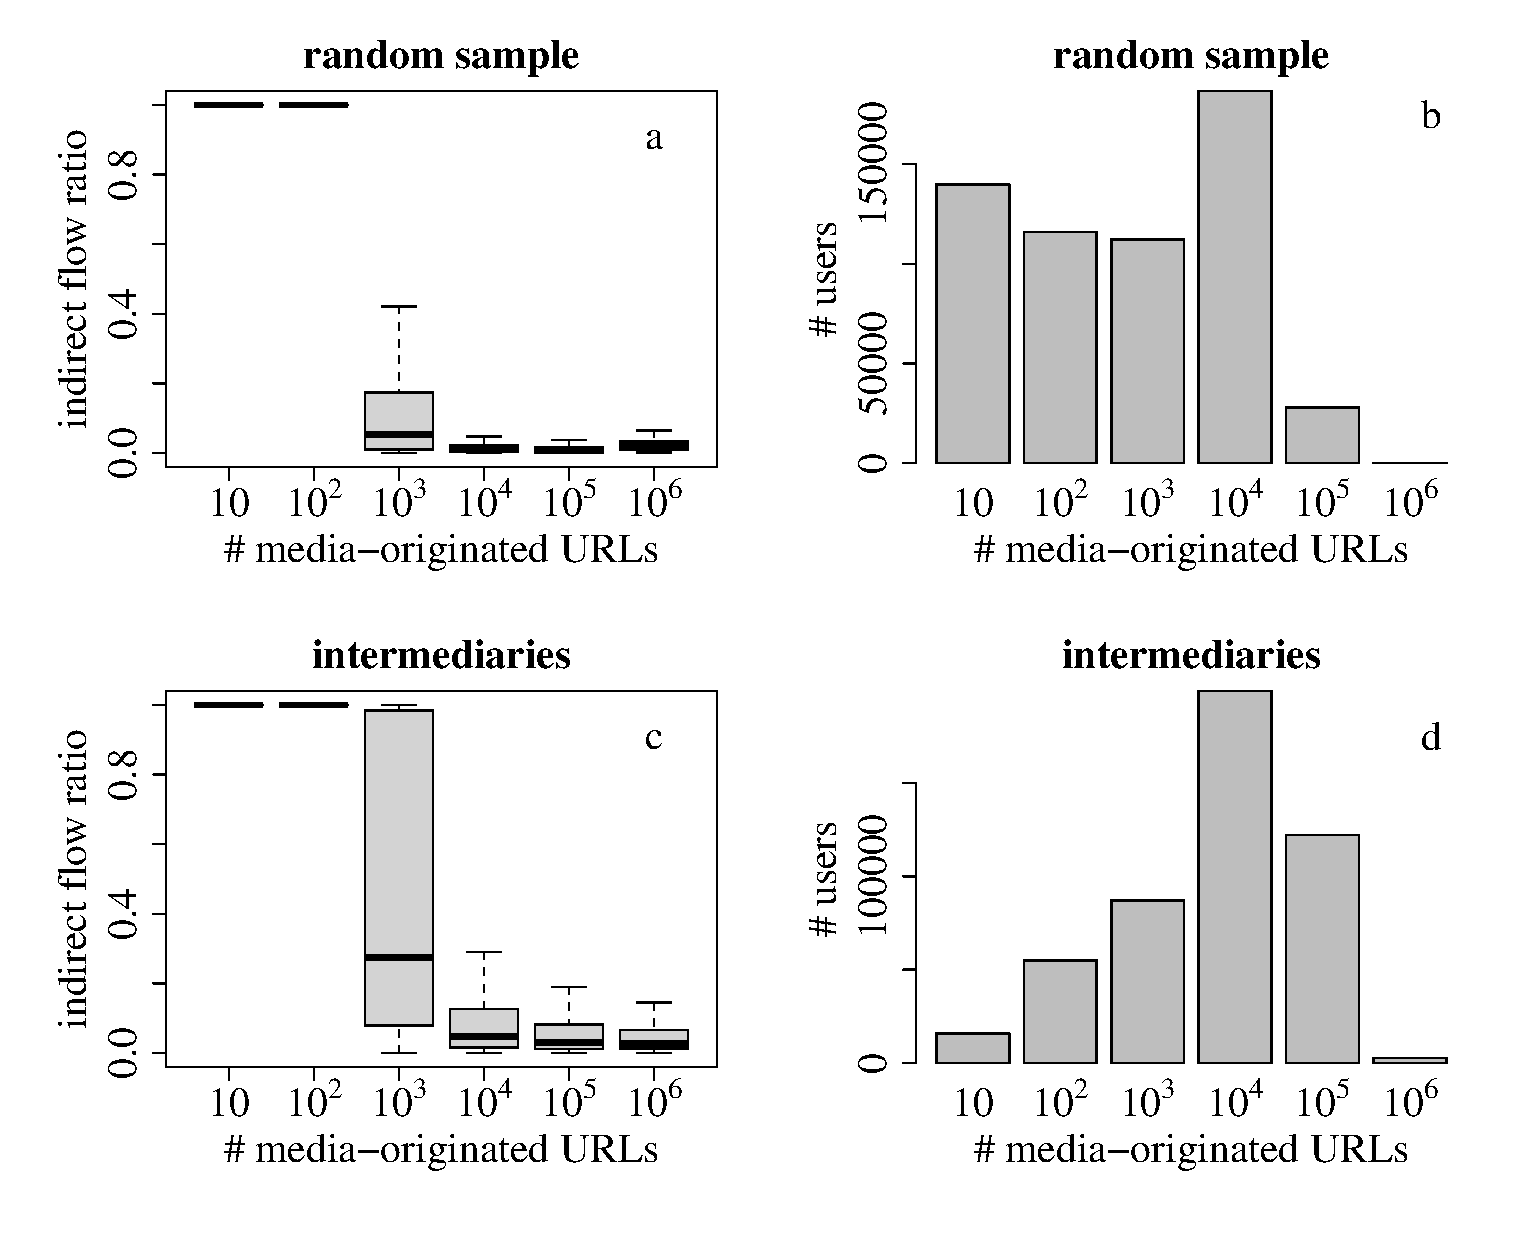
\includegraphics[width=5in]{figures/1M_random_sample_two_step_flow_ratio.eps}
\caption{Percentage of information that received via an
  intermediary as a function of total volume of media content to which
  a user is exposed}
\label{fig:two_step_volume}
\end{figure}

% ======= 
% Differentiating these opinion leaders from ordinary users, however, is
% difficult. To begin with, Table ~\ref{rt_breakdown} shows that very few
% URLs are RT'd by any elite category; thus the bulk of the retweeting and
% reintroduction that we observe is attributable to users we have
% classified as ordinary. Conceivably, our classification scheme above has
% omitted an important category; that is, within the current ``other''
% category may be hidden additional categories of opinions.  As Figure
% \ref{top_k_volume_other} shows, however, even the top 10,000 of these
% users who retweeted the most accounts for a negligible fraction of
% attention among the remaining population.  To the extent that there
% exists a meaningful population of opinion leaders, therefore, it is
% highly distributed.  In fact, for the above 60K sample of recipients, the
% corresponding population of referrers is 160,000---that is, the set of
% opinion leaders is actually larger than the corresponding population of
% followers. Moreover, as Table \ref{two_step_intermediaries} shows, almost
% all of these intermediaries are ordinary users.


Who are these intermediaries, and how many of them are there? In total, the
population of intermediaries is smaller than that of the users who rely on
them, but still surprisingly large, roughly 490K, the vast majority of
which (484K, or 99\%) are classified as ordinary users, not elites. To
illustrate the difference, we note that whereas the top 20K elite users
collectively account for nearly 50\% of attention, the top 10K
most-followed ordinary users account for only 5\%.
% the 480K ``ordinary'' intermediaries account for only ????\%
%%DJW Need to fill in this number, which I think Shaomei calculated at some
%% point SW(1/22/11): I can't find this number for 480K intermediaries in
%% my blog. Duncan, do you think it's in one of the emails? can you search
%% your inbox? If we can't get the exact number, can we somehow assume it
%% is small based on the relatively small attention attracted by the top
%% ordinary users?
Moreover, Figure~\ref{fig:two_step_volume}c also shows that at least some
intermediaries also receive the bulk of their media content indirectly,
just like other ordinary users.

Comparing Figure~\ref{fig:two_step_volume}a and
~\ref{fig:two_step_volume}c, however, we note that intermediaries are not
like other ordinary users in that they are exposed to considerably more
media than randomly selected users (9165 media-originated URLs on average
vs. 1377),
%% DJW: more numbers to fill in.
hence the number of intermediaries who rely on two-step flows is smaller
than for random users. In addition, we find that on average intermediaries
have more followers than randomly sampled users (543 followers versus 34)
and are also more active (180 tweets on average, versus 7). Finally,
Figure~\ref{fig:opinion_leadership} shows that although all intermediaries,
by definition, pass along media content to at least one other user, a
minority satisfies this function for multiple users, where we note that the
most prominent intermediaries are disproportionately drawn from the 4\% of
elite users---Ashton Kucher (aplusk), for example, acts as an intermediary
for over 100,000 users.

% 
% \begin{figure}
% \centering
% \includegraphics[width=3in]{figures/1M_comparison_tweets_followers_opinionleader_ordinaryuser.pdf}
% \caption{Comparison of \# followers and \# tweets for intermediaries and randomly sampled users respectively}
% \label{fig:opinion_leaders_stats}
% \end{figure}


\begin{figure}
\centering
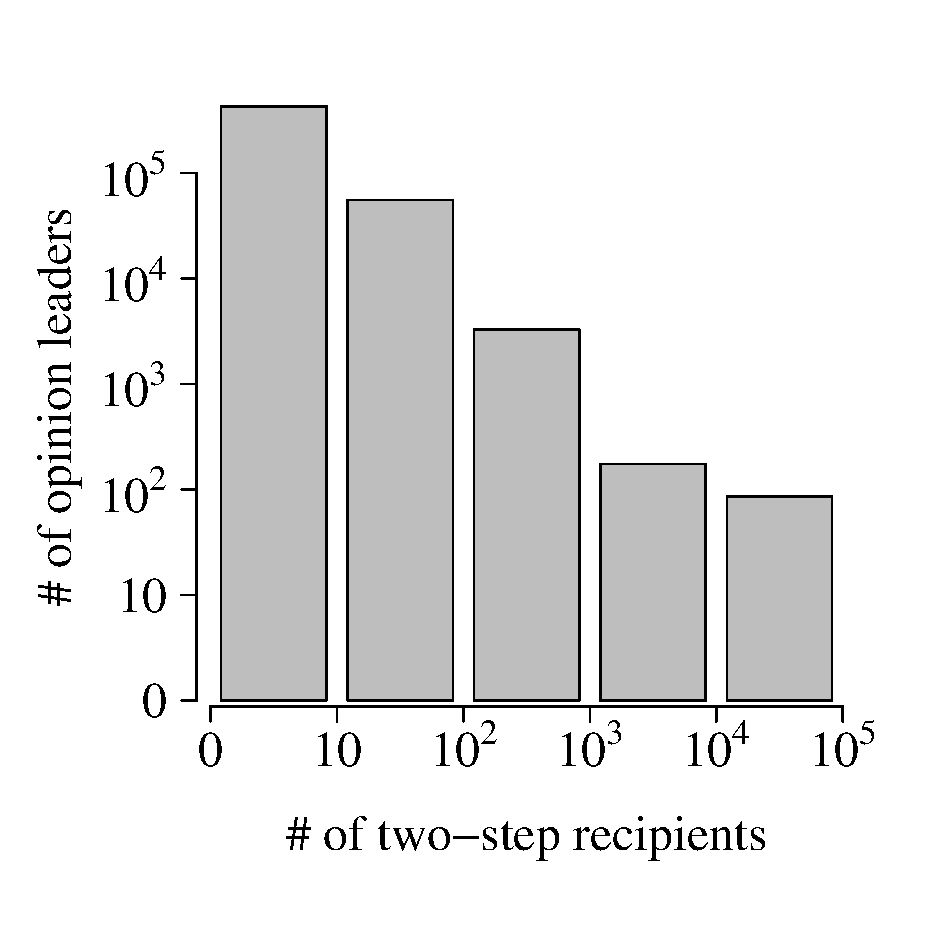
\includegraphics[width=3.5in]{figures/opinion_leader_referral_freq.eps}
\caption{Frequency of intermediaries binned by \# randomly sampled users to whom they transmit media content}
\label{fig:opinion_leadership}
\end{figure}


% Although ordinary in terms of the attention they
% receive, however, intermediaries differ from recipients
% in two respects. First, as Figure \ref{fig:two_step_volume} shows, intermediaries are
% exposed to considerably more media than recipients; and second, they
% receive a larger fraction of media-originating URLs directly from media
% sources (although they are themselves the recipients of referred links
% 26\% of the time).

% These results stand in contrast with the recent marketing literature,
% which has tended to emphasize the importance of a few ``special
% people'' in promoting social change \ref{gladwell}. 

% In terms of the volume of information received, therefore, this result appears to
% support the two-step-flow model of communication~\cite{katz_lazarsfeld},
% which claims precisely that information does not flow directly from the
% media to the masses, but passes first through an intermediate layer of
% ``opinion leaders'' who decide which information to rebroadcast to their
% followers, and which to ignore.

Interestingly, these results are all broadly consistent with the original
conception of the two-step flow, advanced over 50 years ago, which
emphasized that opinion leaders were ``distributed in all occupational
groups, and on every social and economic level,'' corresponding to our
classification of most intermediaries as
ordinary~\cite{katz_lazarsfeld}. The original theory also emphasized that
opinion leaders, like their followers, also received at least some of their
information via two-step flows, but that in general they were more exposed
to the media than their followers---just as we find here. Finally, the
theory predicted that opinion leadership was not a binary attribute, but
rather a continuously varying one, corresponding to our finding that
intermediaries vary widely in the number of users for whom they act as
filters and transmitters of media content.  Given the length of time that
has elapsed since the theory of the two-step flow was articulated, and the
transformational changes that have taken place in communications technology
in the interim---given, in fact, that a service like Twitter was likely
unimaginable at the time---it is remarkable how well the theory agrees with
our observations.

%%DJW: In the abstract and intro we say that we also find some interesting
%%differences.  So either we should specificy some differences, or we
%%should delete the bits where we claim to find them. Do we think there are
%%interesting differences?  500K seems like a lot, but KL don't specify any
%%number, so it's not inconsisent with what they say. Also the blurry
%%boundary between elite and ordinary opinion leaders adds color to the
%%concept, but is again not inconsistent with anything KL said.

\begin{comment}
\begin{table}
\centering
\caption{Referrers of Media-originating URLs}
\label{tab:two_step_intermediaries}
\begin{tabular}{lr}
celeb	& 770 \\ 
media	& 2,796 \\ 
org	& 904 \\ 
blog	& 1,732 \\ 
other	& 152,628 \\
\end{tabular}
\end{table}
\end{comment}

\section{The interaction between people and content}
\label{sec:interaction}
The results in Section~\ref{sec:attention} demonstrate the ``elite'' users
account for a substantial portion of all of the attention on Twitter, but
also show clear differences in how the attention is allocated to the
different elite categories. As illustrated previously, users have natural preferences on content, and influence on Twitter is topic-dependent\cite{Leskovec-EC-2006,Cha-2010}. It is therefore interesting to consider what
kinds of content is being shared by these categories. 

Given the large size of the URL population in our observation period
($260M$), and the large number of ways in which one can classify content
(video vs. text, news vs. entertainment, political news vs. sports news,
etc.), classifying even a small fraction of URLs according to content is an
onerous task. Bakshy et al \cite{bakshy_11}, for example, used Amazon's
Mechanical Turk to classify a stratified sample of 1,000 URLs along a
variety of dimensions; however, this method does not scale well to larger
sample sizes.

Instead, we restrict attention to URLs originated by the New York Times
which, with over 2.5M followers, is the second-most followed news
organization on Twitter after CNN Breaking News. NY Times, however, is
roughly ten times as active as CNN Breaking News, so is a better source of
data. To classify NY Times content, we exploit a convenient feature of
their format---namely that all NY Times URLs are classified in a consistent
way by the section in which they appear (e.g. US, World, Sports, Science,
Arts, etc)
~\footnote{http://www.nytimes.com/year/month/day/category/\\title.html?ref=category}.
Of the 6398 New York Times bit.ly URLs observed, 6370 could be successfully
unshortened and assigned to one of 21 categories. Of these, however, only 9
categories had more than 100 URLs over the observation period, one of
which---``NY region''---was highly specific to the New York metropolitan
area; thus we focused our attention on the remaining 8 topical categories.
Figure \ref{fig:nytimes_categories} shows the overall RT and reintroduction
rates by category. World news is the most popular category, followed by US
news, business, and sports, where increasingly niche categories like
Health, Arts, Science, and Technology are less popular still.  In general,
the overall pattern is replicated for all categories of users, but there
are some minor deviations: In particular, organizations show
disproportionately little interest in business and arts-related stories,
and disproportionately high interest in science, technology, and possibly
world news. Celebrities, by contrast, show greater interest in sports and
less interest in health, while the media shows somewhat greater interest in
US news stories.

% ======= 
% Instead, we adopt a more limited approach. First, we restrict attention
% to URLs originated by one of just two major news organizations, the New
% York Times and CNN; and second, after unshortening all such URLs, we
% exploit a convenient feature of their format---namely that all such URLs
% are classified in a consistent way by the section in which they appear
% (e.g. US, World, Sports, Science, Arts, etc).  For example, all New York
% Times URLs that appear in the business section have the format:
% http://www.nytimes.com/XXXX/XX/XX/business/123abc.html?ref=business,
% while CNN has an analogous structure; thus it is a trivial matter to
% associate all 6,398 NYTimes and 1,804 CNN URLs with the corresponding
% topic section.

\begin{figure}
\centering
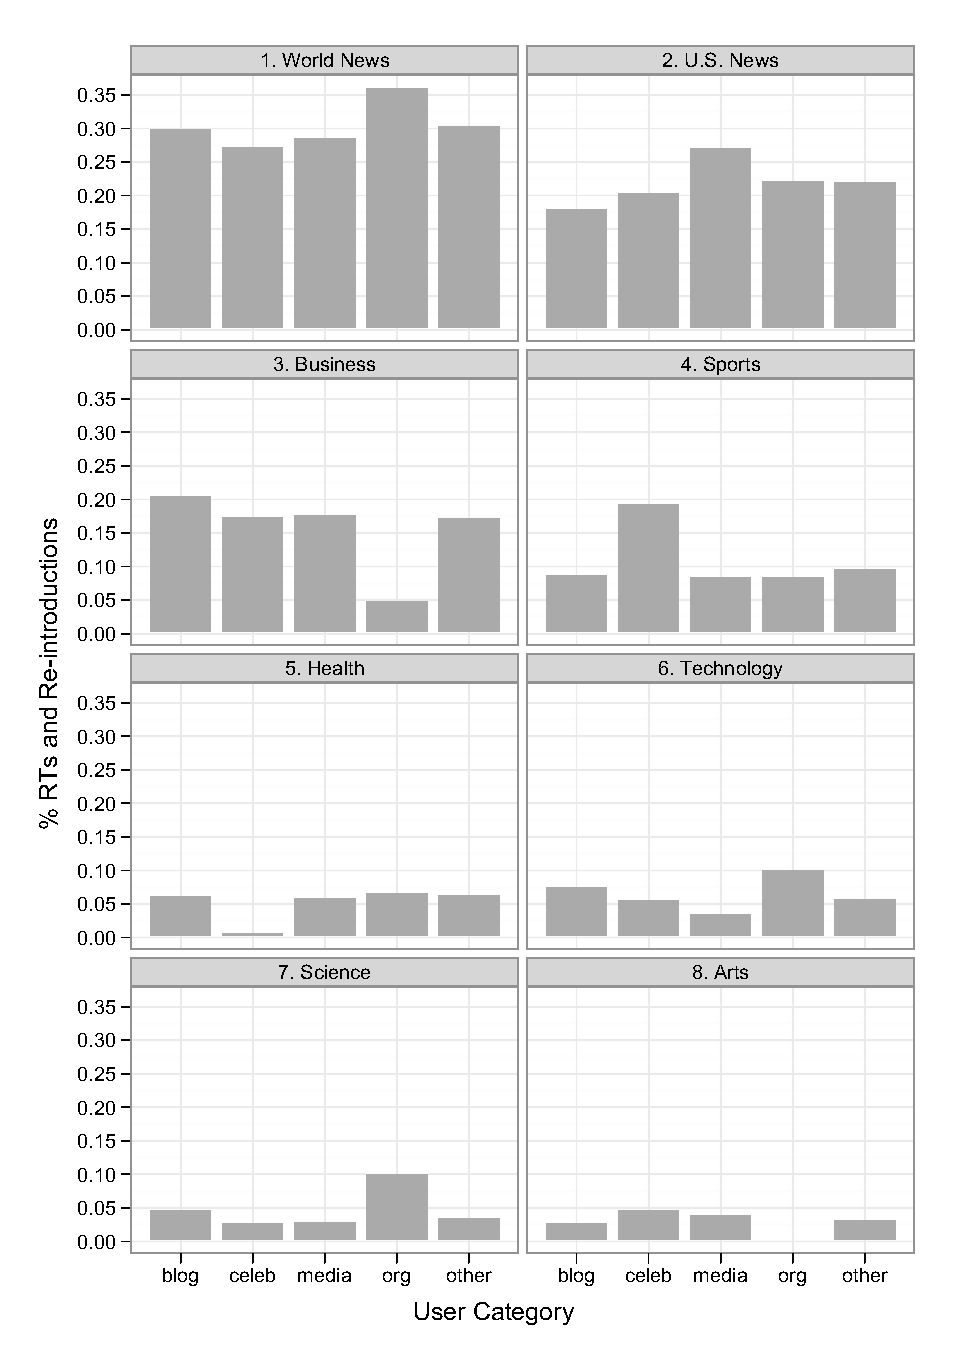
\includegraphics[width=5in]{figures/nyt_url_cat.eps}
\caption{Number of RT's and Reintroductions of New York Times stories by content category}
\label{fig:nytimes_categories}
\end{figure}

In addition, we also consider the accumulated RT/Reintroduction behavior for a
small selection of the most popular URLs. As Figure \ref{fig:popular_URLs}
shows, the link to the official White House blog, which expressed the
administration's initial response to the Haiti earthquake, was rebroadcast
in largely the same manner by all categories of users, as was the
announcement of President Obama winning the Nobel Peace Prize.  By
contrast, the news story announcing the unexpected death of the actress
Brittany Murphy was rebroadcast largely by bloggers, while the breaking
news about Tiger Woods' accident and affair was picked up mostly by the
news media and other celebrities.  Finally, Figure \ref{fig:popular_URLs}
shows two examples of URLs that exhibit very different patterns from news
stories.  First, the URL for DealPlus, a website for ``finding, discussing,
and sharing thousands of deals and coupons for all types of stores,'' was
popular among ordinary users, but almost completely ignored by all
categories of elite users. And second, the video for the song ``Brick by
Boring Brick," by the band Paramore, was again reposted mostly by ordinary
users, but in this case celebrities also reposted it.  Although this
analysis is far from systematic, it suggests that different categories of
users respond to different sorts of content in ways that are consistent
with our classification scheme.

\begin{figure}
\centering
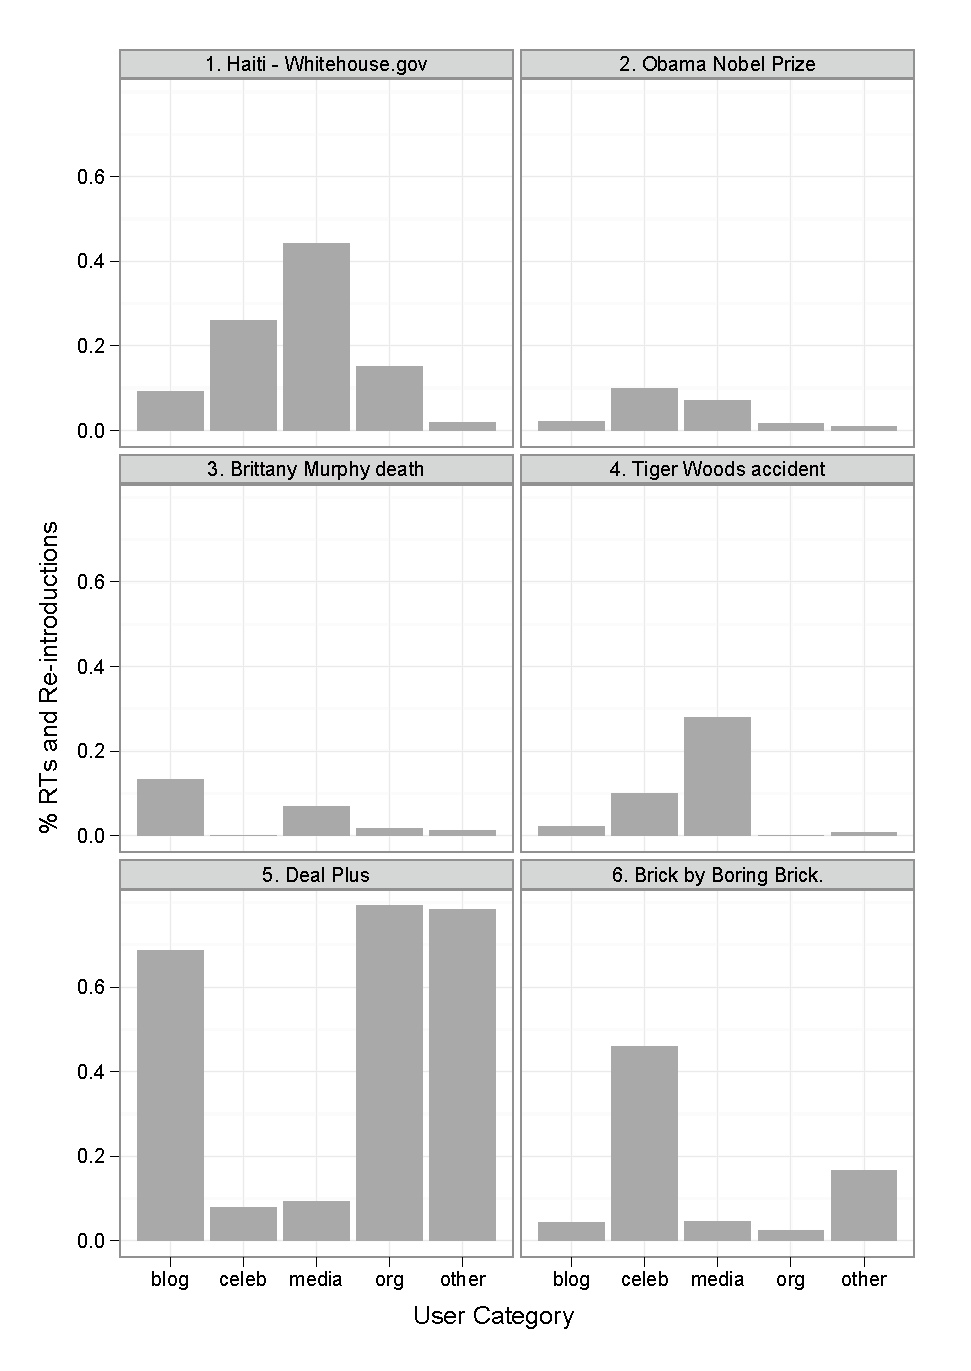
\includegraphics[width=5in]{figures/pop_url_cat_RT.eps}
\caption{Number of RT's and Reintroductions of most popular URLs originating from media and other}
\label{fig:popular_URLs}
\end{figure}

\section{Lifespan of content by category}
\label{sec:lifespan}
% Returning the motivating question in Section \ref{introduction}, ``who
% says what to whom with what effect,'' we now address the issue of
% effects. As noted in Section \ref{introduction} the nature of the data
% available precludes observing the kinds of effects, such as voting or
% purchasing behavior, that communications researchers have been most
% interested in. Nevertheless, we can consider a more limited type of
% effect--namely the duration for which information persists.

% In the second part of our study, we investigate the effect of the
% originating category on.  \begin{itemize} % DW: Already covered in
% previous section \item How much information first introduced by each
% category is retweeted and reintroduced by other categories?  \item How
% does the originating category relate to the lifespan and success of a
% URL?  \item For certain special cases where we can also classify the
% content of a URL, how does content type modify the above?  \end{itemize}

In addition to different types of content, URLs introduced by different
types of elite users or ordinary users may exhibit different lifespans,
by which we mean the time lag between the first and last appearance of a
given URL on Twitter.

Naively, measuring lifespan seems a trivial matter; however, a finite
observation period---which results in censoring of our
data---complicates this task. In other words, a URL that is last observed
towards the end of the observation period may be retweeted or reintroduced
after the period ends, while correspondingly, a URL that is first observed
toward the beginning of the observation window may in fact have been
introduced before the window began. What we observe as the lifespan of a
URL, therefore, is in reality a lower bound on the lifespan. Although
this limitation does not create much of a problem for short-lived
URLs---which account for the vast majority of our observations---it does potentially
create large biases for long lived URLs. In particular, URLs that appear
towards the end of our observation period will be systematically classified
as shorter-lived than URLs that appear towards the beginning.

%%DW: Insert Figures: () schematic of window estimation procedure; (b) tau vs delta tau


\begin{figure}
\centering
\subfigure{
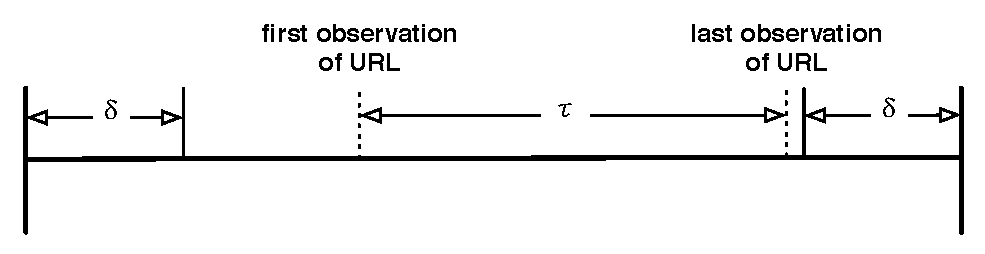
\includegraphics[width=5in]{figures/window_estimation_scheme.eps}
\label{fig:censoring_a}
}
\subfigure{
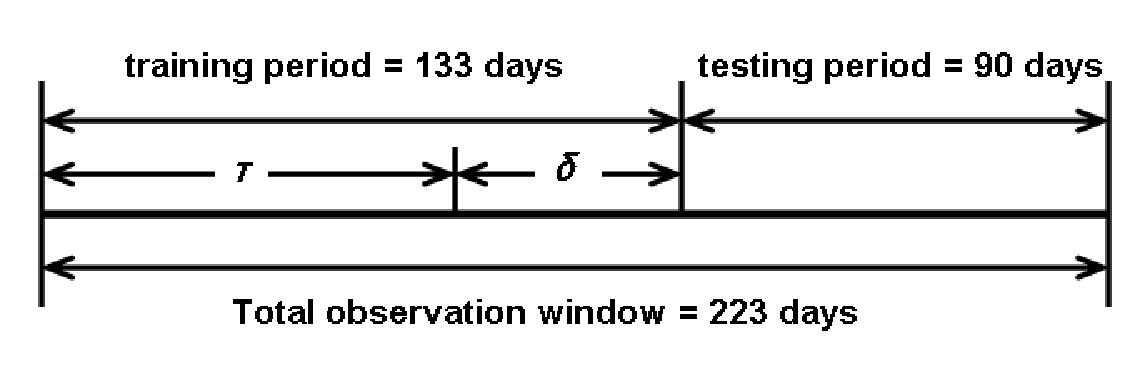
\includegraphics[width=5in]{figures/window_estimation_procedure_scheme.eps}
\label{fig:censoring_b}
}
\caption{(a) Definition of URL lifespan $\tau$ (b) Schematic of lifespan estimation procedure}
\label{fig:censoring}
\end{figure}
% 
% \begin{figure}
% \centering
% 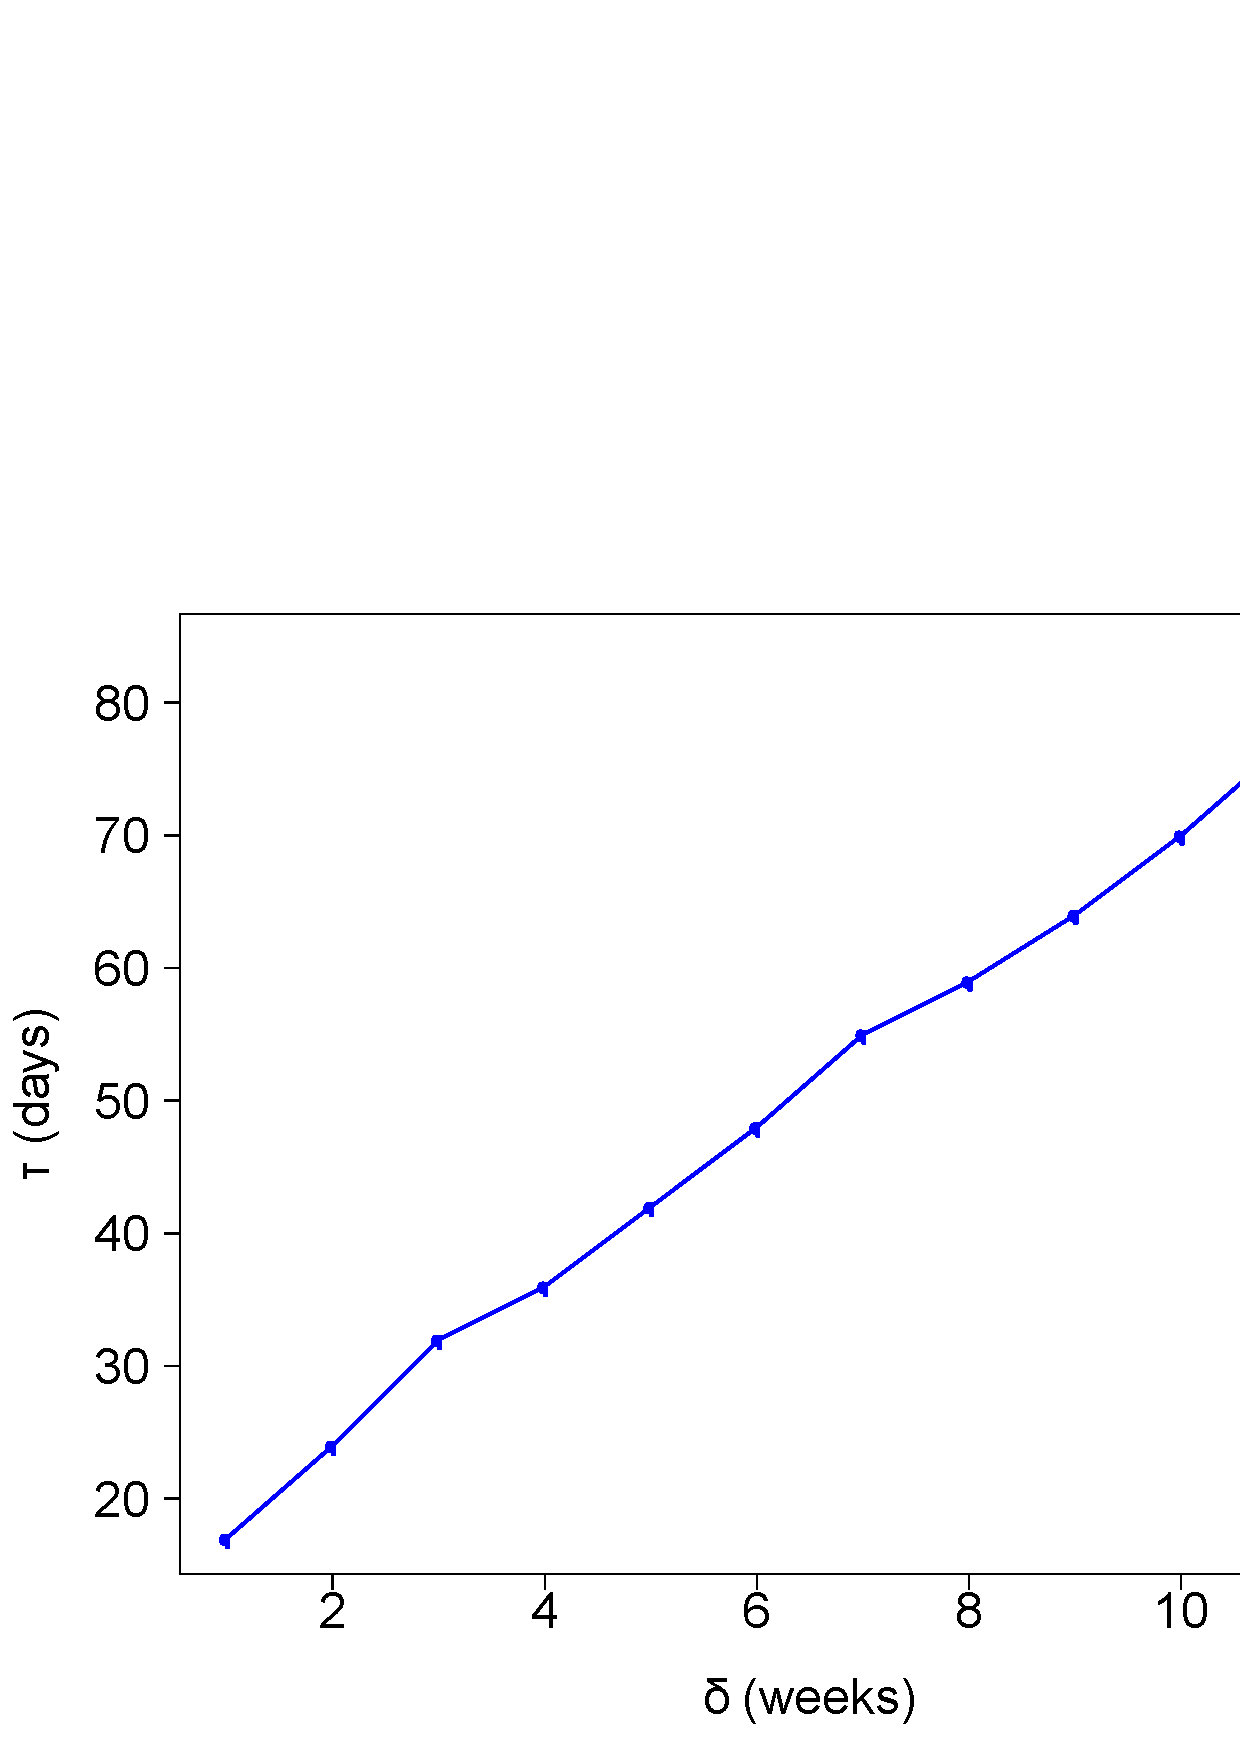
\includegraphics[width=3in]{figures/tau_delta.pdf}
% \caption{Upperbound of $\tau$ with confidence level $>$ 0.95, as a function of $\delta$.}
% \label{fig:tau_v_delta}
% \end{figure}

To address the censoring problem, we seek to determine a buffer
$\delta$ at both the beginning and the end of our $223$-day period,
and only count URLs as having a lifespan of $\tau$ if (a) they do not
appear in the first $\delta$ days, (b) they first appear in the
interval between the buffers, and (c) they do not appear in the last
$\delta$ days, as illustrated in Figure~\ref{fig:censoring_a}.
% That is, we seek a value for $\delta$ which balances the
% number of URLs whose lifetimes we report with the degree of accuracy
% to which these lifespans can be estimated.
To determine $\delta$ we first split the $223$ day period into two
segments---the first 133 day estimation period and the last 90 day
evaluation period (see Figure~\ref{fig:censoring_b})---and then ask: if we
(a) observe a URL first appear in the first $(133 - \delta)$ days and (b) do
not see it in the $\delta$ days prior to the onset of the evaluation period, how likely
are we see it in the last 90 days?  Clearly this depends on the actual
lifespan of the URL, as the longer a URL lives, the more likely it will
re-appear in the future. Using this estimation/evaluation split, we find an
upper-bound on lifespan for which we can determine the actual lifespan with
$95 \%$ accuracy as a function of $\delta$. Finally, because we require a
beginning and ending buffer, and because we can only classify a URL as
having lifespan $\tau$ if it appears at least $\tau$ days before the end of
our window, we need to pick $\tau$ and $\delta$ such that $\tau + 2\delta
\leq 223$. We determined that $\tau = 70$ and $\delta=70$ sufficiently
satisfied our constraints; thus for the following analysis, we consider
only URLs that have a lifespan $\tau \leq 70$~\footnote{We also performed our analysis with different values of $\tau$, finding very similar results; thus our conclusions are robust with respect to the details of our estimation procedure.}.


\begin{figure}[ht]
\centering
\subfigure[Count]{
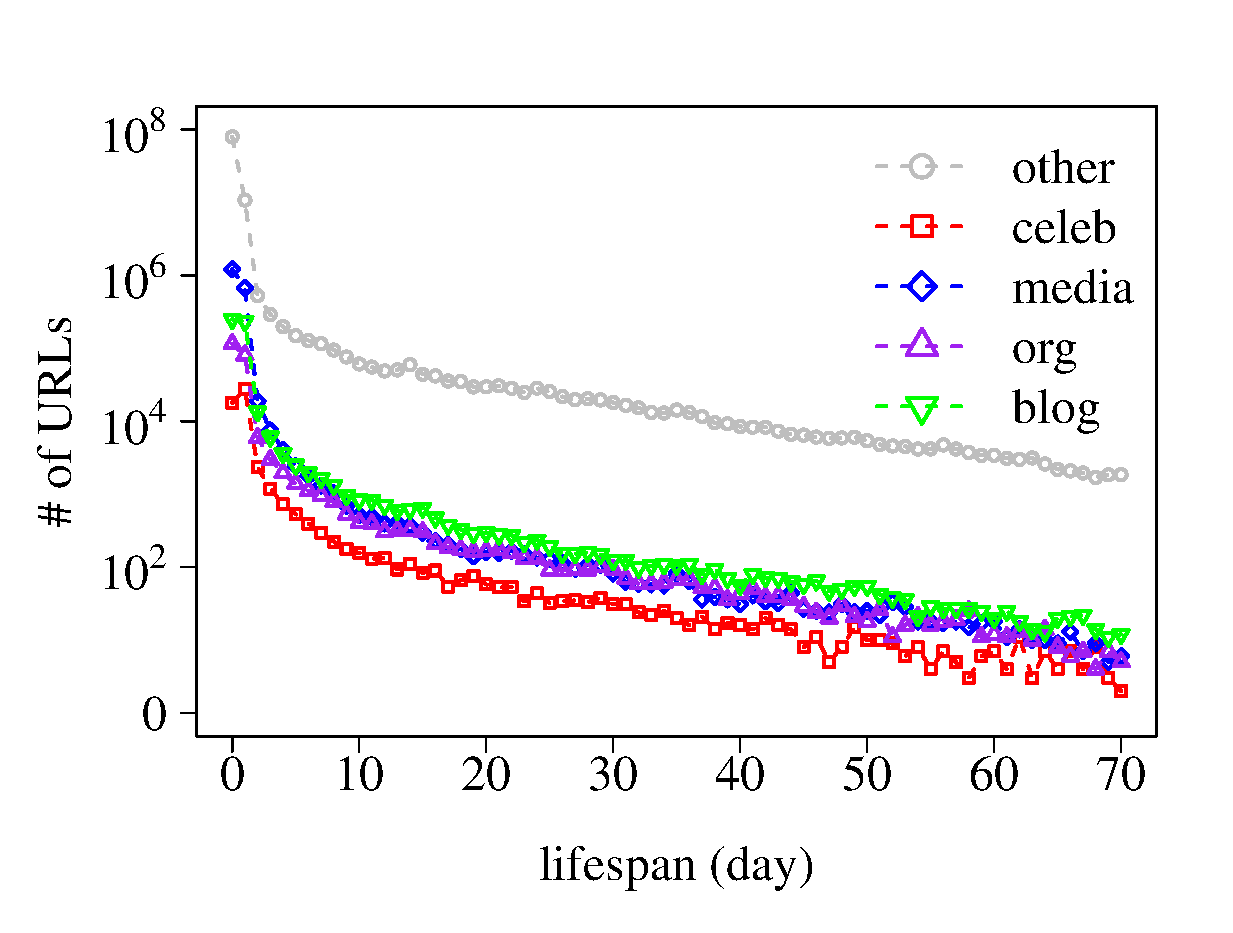
\includegraphics[width=3.5in]{figures/url_lifespan_by_categories_500K_censored.eps}
\label{fig:lifespan_category}
}
\subfigure[Percent]{
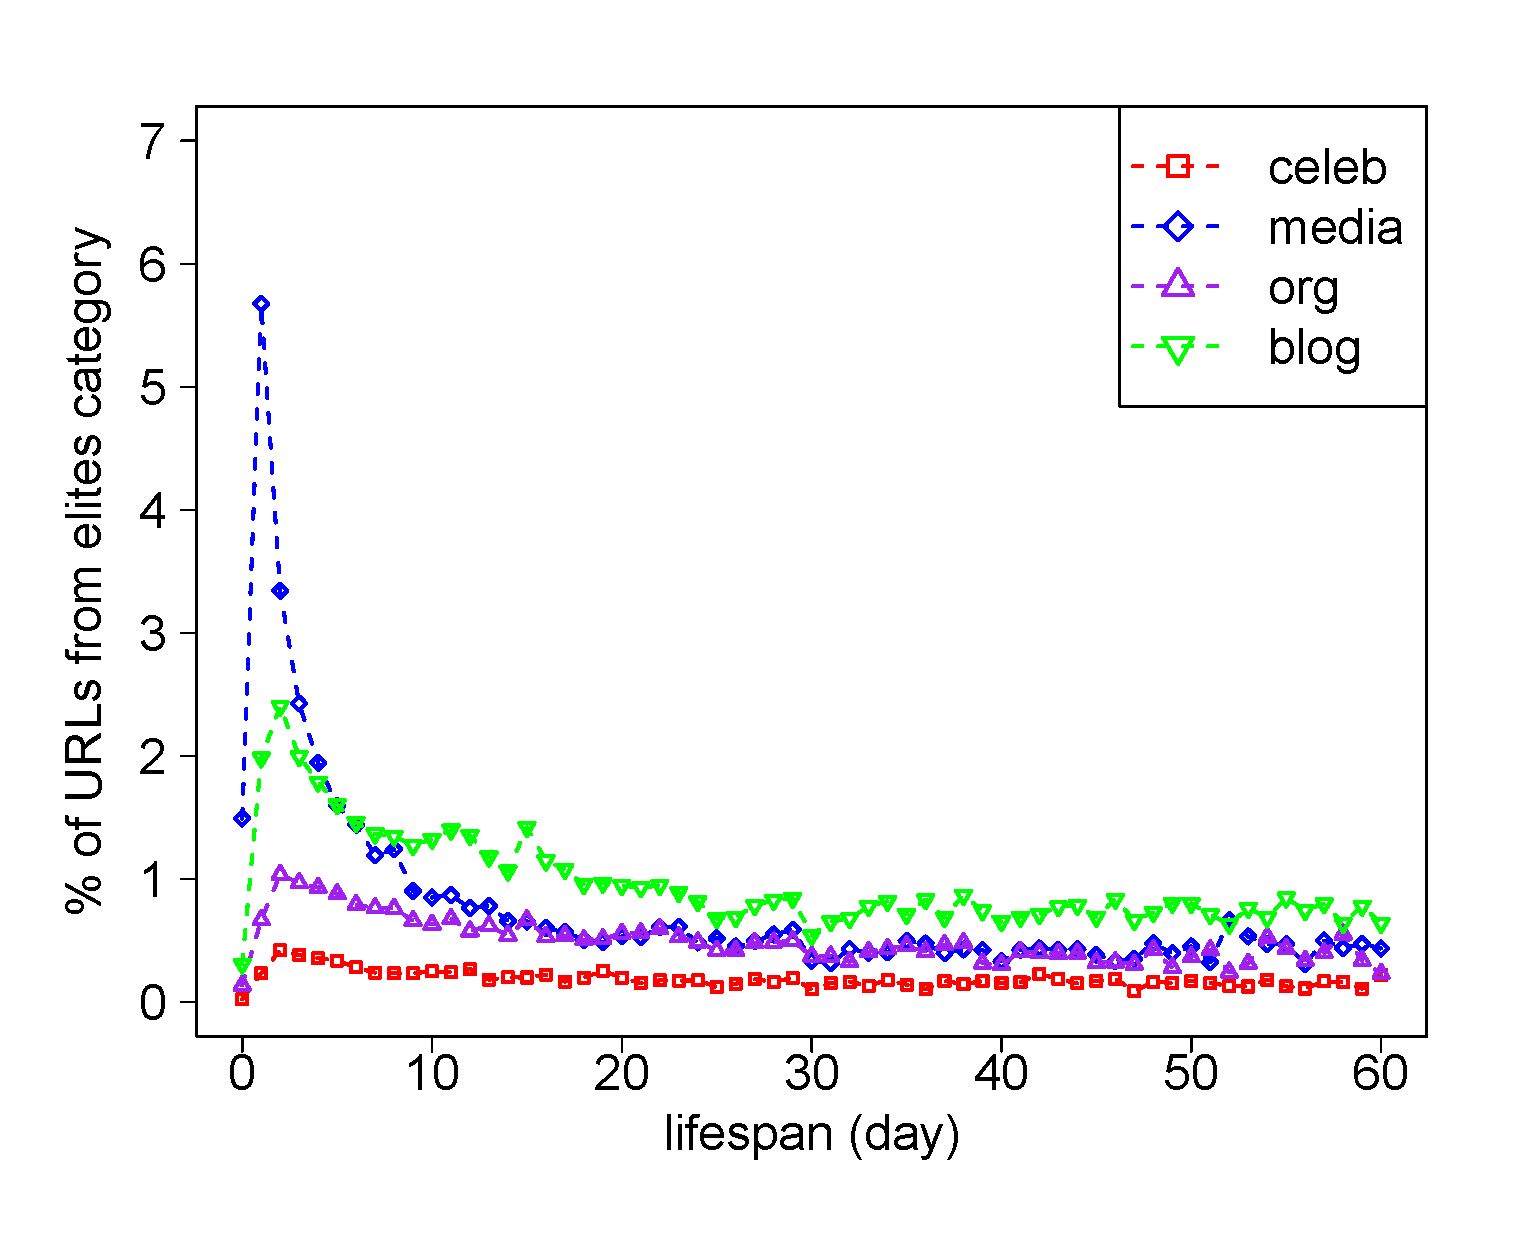
\includegraphics[width=3.5in]{figures/url_lifespan_percentage_by_categories_500K_censored.eps}
\label{fig:lifespan_percentage_category}
}
\caption{(a) Count and
  (b) percentage of URLs initiated by
  4 categories, with different lifespans}
\label{fig:lifespan}
\end{figure}


\begin{figure}[ht]
\centering
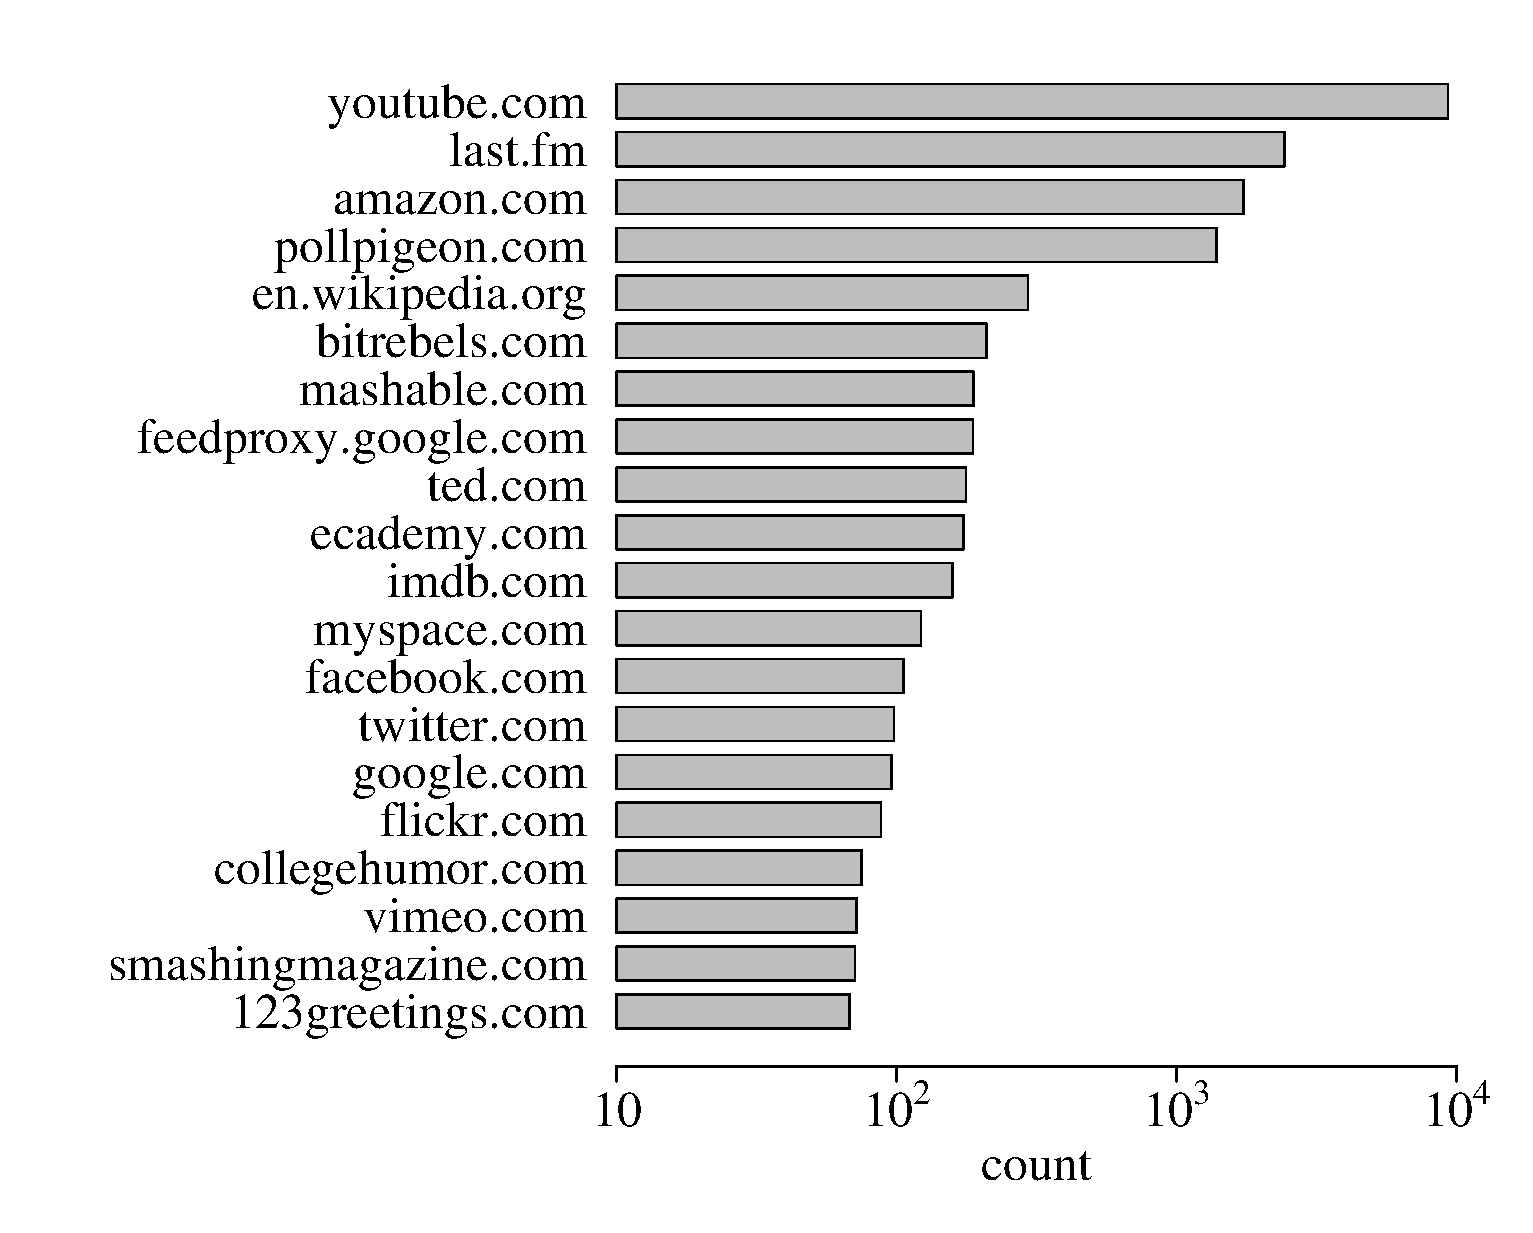
\includegraphics[width=5in]{figures/domains_breakdown_longlived_urls.eps}
\caption{Top 20 domains for URLs that lived more than 200 days}
\label{fig:longlived_urls}
\end{figure}

Having established a method for estimating URL lifespan, we
now explore the lifespan of URLs introduced by different categories of
users, as shown in Figure \ref{fig:lifespan_category}.
% \footnote{This
%   figure only shows URLs that appeared in our dataset more than once.
%   The majority of the URLs (220M) appeared only once, which is 10
%   times as many URLs as had a lifespan of only a day.}.
%
URLs initiated by the elite categories exhibit a similar distribution over
lifespan to those initiated by ordinary users. As Figure
\ref{fig:lifespan_percentage_category} shows, however, when looking at the
percentage of URLs of different lifespans initiated by each category, we
see two additional results: first, URLs originated by media actors generate
a large portion of short-lived URLs (especially URLs with $\tau=0$, those
that only appeared once); and second, URLs originated by bloggers are
overrepresented among the longer-lived content.  Both of these results can
be explained by the type of content that originates from different sources:
whereas news stories tend to be replaced by updates on a daily or more
frequent basis, the sorts of URLs that are picked up by bloggers are of
more persistent interest, and so are more likely to be retweeted or
reintroduced months or even years after their initial introduction.
Twitter, in other words, should be viewed as a subset of a much larger
media ecosystem in which content exists and is repeatedly rediscovered by
Twitter users. Some of this content---such as daily news stories---has a
relatively short period of relevance, after which a given story is unlikely
to be reintroduced or rebroadcast. At the other extreme, classic music
videos, movie clips, and long-format magazine articles have lifespans that
are effectively unbounded, and can seemingly be rediscovered by Twitter
users indefinitely without losing relevance.

To shed more light on the nature of long-lived content on Twitter, we used
the bit.ly API service to unshorten 35K of the most long-lived URLs (URLs
that lived at least 200 days), and mapped them into 21034 web domains. As
Figure \ref{fig:longlived_urls} shows, the population of long-lived URLs is
dominated by videos, music, and consumer goods.  
Two related points are illustrated by Figure
\ref{fig:RT_lifespan_category}, which shows the average RT rate (the
proportion of tweets containing the URL that are retweets of another tweet)
of URLs with different lifespans, grouped by the categories that introduced
the URL\footnote{Note here that URLs with lifespan = 0 are those URLs that
  only appeared once in our dataset, thus the RT rate is zero.}.
%
First, for ordinary users, the majority of appearances of URLs after the
initial introduction derives not from retweeting, but rather from
reintroduction, where this result is especially pronounced for long-lived
URLs.  For the vast majority of URLs on Twitter, in other words, longevity
is determined not by diffusion, but by many different users independently
rediscovering the same content, consistent with our interpretation above.
% above that certain types of online content retain their relevance
% indefinitely, and their persistence on Twitter is driven mostly by users
% rediscovering content outside of the Twitter ecosystem.
Second, however, for URLs introduced by elite users, the result is somewhat
the opposite---that is, they are more likely to be retweeted than
reintroduced, even for URLs that persist for weeks.  Although it is
unsurprising that elite users generate more retweets than ordinary users,
the size of the difference is nevertheless striking, and suggests that in
spite of the dominant result above that content lifespan is determined to a
large extent by the type of content, the source of its origin also impacts
its persistence, at least on average---a result that is consistent with
previous findings~\cite{bakshy_11}.

\begin{figure}
\centering
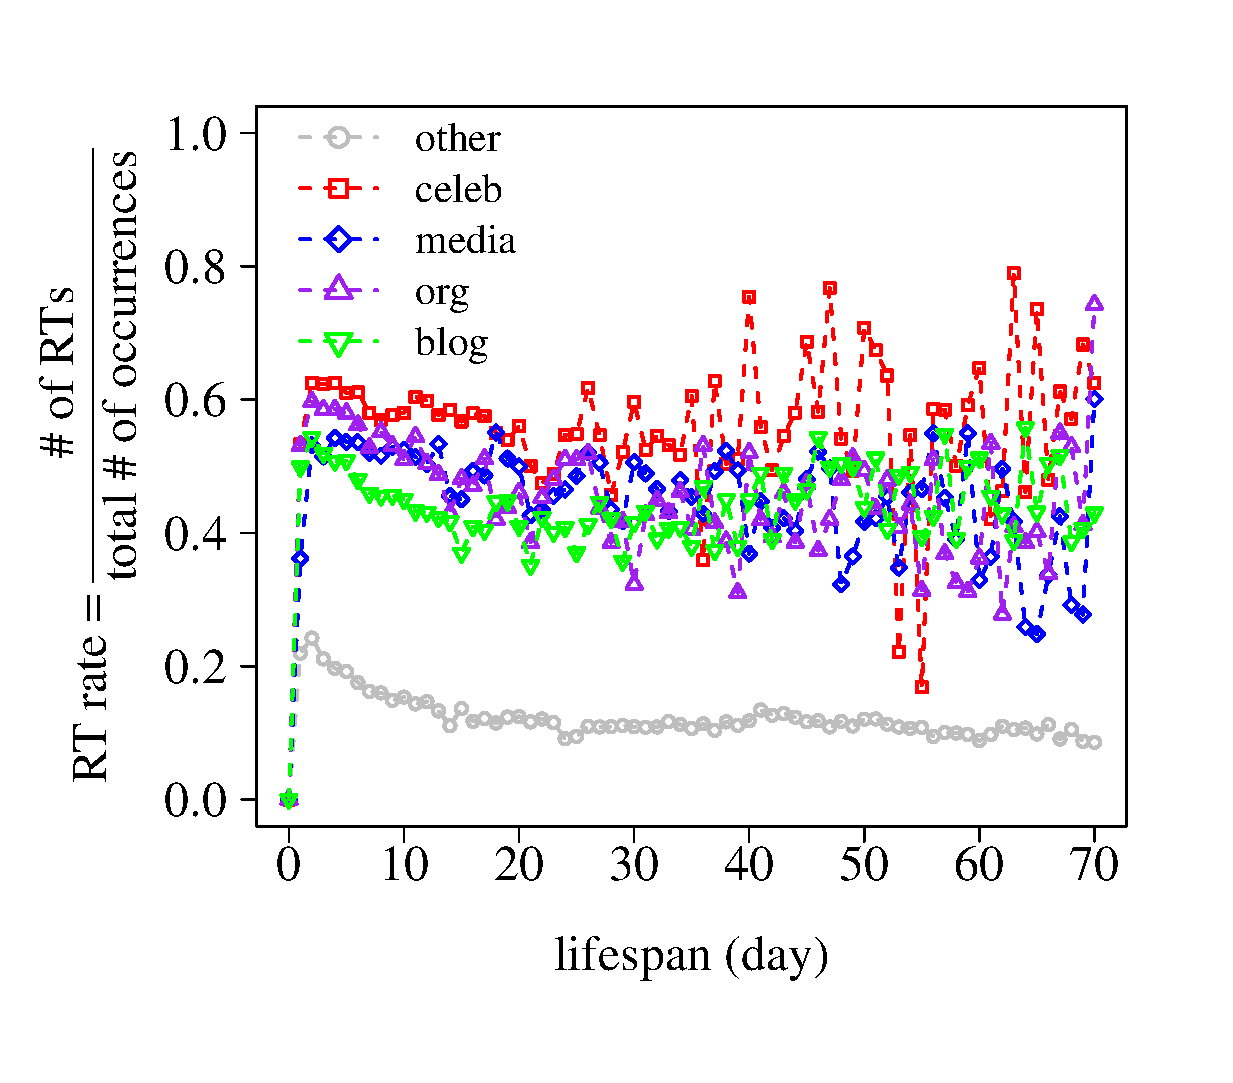
\includegraphics[width=4in]{figures/url_lifespan_RTrate_by_categories_500K_censored.eps}
\caption{Average RT rate by lifespan for each of the originating categories}
\label{fig:RT_lifespan_category}
\end{figure}


\section{Conclusion}
\label{sec:conclusion}
In this chapter, we investigated the influencer problem by incorporating exogenous influence into the context of Twitter.  
In particular, we find that although audience attention has indeed fragmented among
a wider pool of content producers than classical models of mass media,
attention remains highly concentrated, where roughly 0.05\% of the population
accounts for almost half of all posted URLs.  Within this
population of elite users, moreover, we find that attention is highly homophilous, with
celebrities following celebrities, media following media, and bloggers
following bloggers.  Second, we find considerable support for the two-step
flow of information---almost half the information that originates from the
media passes to the masses indirectly via a diffuse intermediate layer of
opinion leaders, who although classified as ordinary users, are more
connected and more exposed to the media than their followers.  Third, we
find that although all categories devote a roughly similar fraction of
their attention to different categories of news (World, U.S., Business,
etc), there are some differences---organizations, for example, devote a
surprisingly small fraction of their attention to business-related news.
% We also find that certain types of popular URLs attract quite
% different levels of attention from different categories, reflecting
% their distinct interests. 
We also find that different types of content exhibit very different
lifespans: media-originated URLs are disproportionately represented among
short-lived URLs while those originated by bloggers tend to be
overrepresented among long-lived URLs. Finally, we find that the
longest-lived URLs are dominated by content such as videos and music, which
are continually being rediscovered by Twitter users and appear to persist
indefinitely. We will further investigate the role of content in the diffusion process in next chapter.

By restricting our attention to URLs shared on Twitter, our conclusions are
necessarily limited to one narrow cross-section of the media landscape.  An
interesting direction for future work would therefore be to apply similar
methods to quantifying influence via more traditional channels, such
as TV and radio on the one hand, and interpersonal interactions on the
other hand.  Moreover, although our approach of defining a limited set of
predetermined user-categories allowed for relatively convenient analysis
and straightforward interpretation, it would be interesting to explore
automatic classification schemes from which additional user categories
could emerge.
%In particular, such an approach would allow one to examine the category of
% opinion leaders in more detail, possibly identifying opinion leaders for
% different topics, as has been proposed elsewhere ~\cite{weimann_94}.

%Finally, another two areas for future work are first, to extract content information in a more systematic manner---the ``what'' of Lasswell's maxim; and second, to focus more on the effects of communication by merging the data regarding information flow on Twitter with other sources of outcome data, such as the opinions or actions of the recipients of the information.


\chapter{The role of content}
\label{chap:content}
As shown in previous chapter, the content originated by different people exhibit different lifespan, however, the connection between content and authors are relatively weak thus does not have much predictive power (for example, bloggers can write about a variety of things). In this chapter, we present a large scale empirical study directly on the textual content in relationship to the perisistence of information. Our goal is to look for intrinsic qualities of the content that effectively affect the dissemination process, especially, resulting in different lifespans of information. We make two main contributions:
\begin{itemize}
% (this is method but not contribution)\item We find power-law in the distribution of the lastingness of webpages and then formalize the problem into a binary classification problem.
\item We build a classifier that predicts the decay/persistence of information with textual features, providing one of the first empirical studies of the connection between content and temporal variations of information in online social media.
\item We investigate the properties of the text that are associated
with different temporal patterns, finding significant differences in
word usage and sentiment between rapidly-fading and long-lasting information.
\end{itemize}

In the following sections of this chapter, we first provide an overview of the data we are using for this study, then present a binary classifier that predicts the persistence of URLs, using texual features from webpages pointed to by the URLs. We further examine and discuss different aspects of the content that are correlated with the difference in temporal patterns. In the end, we provide some additional insights about the quality of YouTube videos in relationship to the decay time.

\section{Data}

\subsection{Summary}
In this study, we used the dataset publicly shared by the authors of \cite{Yang-2011}\footnote{http://snap.stanford.edu/data/twitter7.html}, 
consisting of approximately $20\%$-$30\%$ of all the tweets generated between June 1, 2009 and December 31, 2009. 
%Since it is collected over a continuous period of time, this dataset is desirable to study the temporal patterns of information. 
We only study the temporal patterns of bit.ly URLs for two reasons, 
following the arguments of \cite{Wu-Twitter-2011}. First, 
shortened URLs have a unique token that is easily traceable in individual tweets. 
Second, the associated webpages provide a much richer source of content beyond the 140-character limit of tweets. 
From the total 476M tweets contained in the dataset, we find 118M distinct URLs embedded in 186M tweets. 
Among all the URLs, nearly half of them (56M) are bit.ly URLs (i.e., start with http://bit.ly/). 
For simplicity, we only extract the time series of bit.ly URLs and use them as a representative sample of all temporal patterns. 
Considering that a large portion of URLs mentioned in Twitter are spam and may not be able to provide meaningful content, 
we restrict our study to the bit.ly URLs that appeared more than 10 times in retweets \footnote{We recognize a post as retweet when it contains ``RT @'' or ``via @''.}, 
which gives us 131K bit.ly URLs. 
We are able to crawl 117K webpages pointed to by these bit.ly URLs, the remaining 14K URLs that we fail to crawl are mostly misspelled 
or linked to webpages that no longer exist. 

%% possibly move to the next section?
We further restrict our study to URLs that are mentioned more than 50 times in order to remove spam and have sufficient observations to measure temporal dynamics, which leaves us with 21K URLs. 
In the rest of this paper, when we talk about URLs and temporal patterns, we mean these 21K bit.ly URLs and the temporal pattern in their time series.

\subsection{Persistence of URLs}
After extracting the data of interest, we first propose a quantitative metric of persistence and present some insights on the overall temporal pattern of the URLs we study.

As the focus of this study is how fast URLs fade, we measure decay rates following peak attention. 
For each URL $u$, let the hour of maximum attention (also called
the peak of attention) be hour $0$. 
Then the {\em decay time} $t_u$ is defined as the hour after the peak 
when the number of mentions first reaches $75\%$ of the total.
Instead of measuring the time lag between the first and last mention of a given URL \cite{Wu-Twitter-2011}, we intentionally choose to measure the time lag from the peak of attention to the point when the URL fades away, as given the limited observation window when the dataset was collected, it is not obvious to determine when exactly a URL was first introduced or last appeared on Twitter.
The distribution of $t_u$ shows heavy tail(see Figure~\ref{fig:tu_distribution}), as found previously in the distribution of URL lifespan\cite{Wu-Twitter-2011}.
%The distribution of $t_u$ approximately follows a power-law (see Figure \ref{fig:tu_distribution}), as found previously in the distribution of URL lifespan \cite{Wu-Twitter-2011}.
Among all URLs we studied, the mean $t_u$ is 217.3  hour and the median $t_u$ is 19 hours.

%\vspace{-0.1in}
\begin{figure}[htb!]
\centering
\epsfig{figure=figures/tu_distribution.eps, width=5in}
%\vspace{-0.3in}
\caption{Distribution of URL decay time $t_u$}
\label{fig:tu_distribution}
\end{figure}

We further examine the relationship between $t_u$ and the overall popularity of URLs. Figure~\ref{fig:tu_tweet_rt} shows the average number of tweets and retweets accumulated by each URL as a function of $t_u$. Given the power-law distribution of $t_u$, we bin URLs by the integer part of $\log_2(t_u)$, and calculate the mean for each bin.  Although the persistent URLs are mentioned in slightly more tweets, the rapidly-fading URLs do better at attracting retweets. This result is consistent with previous findings that the longevity of information is determined not by diffusion, but by independent generation of tweets of the same content over time \cite{Wu-Twitter-2011}.

%\vspace{-0.1in}
\begin{figure}[htb!]
\centering
\epsfig{figure=figures/tu_rt_tweet.eps, width=5in}
%\vspace{-0.3in}
\caption{URL overall popularity as a funtion of $t_u$}
\label{fig:tu_tweet_rt}
\end{figure}


\section{Predicting temporal patterns based on content}
In this section, we formally define the temporal pattern classification task and present our findings.

\subsection{Identifying information with two distinct temporal patterns}
We start by casting our question into a binary classification problem
in which class 1 is defined as consisting of those
URLs with $t_u < 6$ and class 0 is defined
defined as consisting of those
URLs with $t_u > 24$. In this way we get a positive class
with 7042 examples and a negative class with 6185 examples. We exclude
the 7K examples in the middle, as the data is much noisier and the
persistence of these URLs is ambiguous --- our goal in this first
exploration of persistence prediction is to construct a 
well-defined and tractable task from which we can understand whether there
are features that meaningfully separate rapidly-fading URLs
from long-lasting ones.
 

%    To study whether the content of webpage is related with its temporal pattern, as we have introduced in the Section \ref{sec:data}, we take the two distinct temporal patterns and formalize the problem into a binary classification.

%    To elaborate, we take the peak hour of attention as the signal that the hottest time point of the webpage, denoted as time $0$. Starting from the peak, we define the hour when  \# of tweets containing the url reaches $75\%$ of the total volume we observed as the signal that this webpage has faded away, denoted as hour $t$.

%    As for labeling each webpage, according to our observation, we take the urls with $t < 6$ and $t > 24$ as two distinct temporal patterns and label them as following:

%\begin{itemize}
%\item $t < 6$: urls die fast in this class. They tend to be soon ignored after they get attention.They are labeled as positive class (+).
%\item $t > 24$: urls last much longer in this class. They receive continuous attention.We label them as negative class (-).
%\end{itemize}

%Details about the number of instances in each class are shown in \ref{tb:classnumber}

%\begin{table}
%\caption{Number of Instances}
%\label{tb:classnumber}
%\centering
%\begin{tabular}{|c|c|c|}
%\hline
%& Positive & Negative \\
%\hline
%Number & 6185 & 7042 \\
%\hline
%\end{tabular}
%\end{table}

To better illustrate our classification scheme, we apply the time series normalization method introduced in \cite{Yang-2011} and calculate the centroid of time series for each class, as shown in Figure \ref{fig:classexample}. The two classes we define do in fact collectively exhibit very different temporal patterns: URLs of the positive class fade away slowly, with periodic, multiple peaks of attention; URLs of the negative class have a single spike and a rapid decay afterwards.
 

%Figure \ref{fig:classexample} shows the temporal pattern of the centroid in the two classes. (generated according to the method introduced in [Yang and Leskovec 2011].)

%\vspace{-0.1in}
\begin{figure}[htb!]
\centering
\epsfig{figure=figures/class_centroids.eps, width=5in}
\caption{Normalized time series centroids for two classes}
\label{fig:classexample}
%\vspace{-0.2in}
\end{figure}

\subsection{Features}
To predict the temporal class of URLs, we extract and experiment with the following four incremental sets of unigram features from the HTML webpages linked by the URLs (one-character tokens and those that consist only of numbers are filtered out):

\begin{itemize}
\item Header. The text in the header of HTML, within tags ``$<$title$>$'',``$<$description$>$'', and ``$<$keywords$>$''. 
\item Header + URL.  In addition to Header, this feature set also uses the terms tokenized from the URL links embedded in the HTML (i.e.,within ``$<$href$>$'' ). 
\item Header + Body. In addition to Header, this feature set includes all the text in the body of HTML. 
\item Header + URL + Body. This feature set combines all the features mentioned above. 
\end{itemize}

As mentioned above, to get more meaningful unigram features, after tokenizing all the textual content into word terms, we filter the terms with length 1 (e.g., ``s'', ``t'') and the terms consisting of only numbers. As the dimension increases tremendousely in the last 3 sets of features, we also filter the infrequent terms (i.e., terms with total frequency less than 20). Table \ref{table:feature-sets} gives a summary of the number of features in each set.

\begin{table}[t]
\centering
\caption{Feature size}
\label{table:feature-sets}
\begin{tabular}{c|c}
\hline
 \emph{Feature} & \emph{$\#$ of unique unigram terms} \\
\hline
Header & 18471  \\
\hline
Header + URL & 27433 \\
\hline
Header + Body & 59475 \\
\hline
Header + Body + URL & 76487\\
\hline
\end{tabular}
\end{table}

\subsection{Classifier performance}
To predict the persistence of webpages, we employ a Support Vector Machine (SVM)\footnote{The SVM package we use is SVMLight, \url{http://svmlight.joachims.org/}} classifier with a binary representation of unigram features (if a term appears in a webpage, the corresponding coordinate has value 1, and value 0 otherwise). To work with high-dimensional features, we use the linear SVM kernel for efficiency. 
We also apply the default parameters for SVM classifier for a fair comparison among different sets of features. Table \ref{table:performance} gives the performance of classifiers with different sets of features using 10-fold cross validation. 

%In this part we presents the performance of classifiers. We use svmlight\footnote{http:\\blabla}. To make a fair comparison, we use default parameters, that is, SVM with linear kernel. The performance is shown in Table \ref{tb:performance}. The experiment is generated by 10-fold cross validation in the dataset.

\begin{table}[t]
\caption{Results for predicting lastingness of information}
\label{table:performance}
\centering
\begin{tabular}{c|c|c|c}
\hline
\emph{Feature} & \emph{Accuracy} & \emph{Pos F1} & \emph{Neg F1}\\
\hline
Header & 0.6909 & 0.7399 & 0.6186 \\
\hline
Header + URL & 0.7177 & 0.7666 & 0.6423\\
\hline
Header + Body & 0.7136 & 0.7664 & 0.6296\\
\hline
Header + Body + URL & 0.7224 & 0.7708 & 0.6478\\
\hline
\end{tabular}
\end{table}

Table \ref{table:performance} shows that in general, the simple linear-kernel SVM classifier can predict the persistent/rapidly-fading category of URLs with impressively high accuracy (around $70\%$), as comparedd to $53\%$ for always predicting positive. Also, the F1 score for positive class is around $75\%$, which shows a remarkable balance of precision and recall at identifying the persistent content. This result provides strong evidences for the connection between the content of HTML pages and the persistence of the associated URLs.  Moreover, comparing across 4 feature sets, we see that the more information we have about the content, the better the classifier performs. This finding further confirms the relationship between textual content and the persistence of attention of the information.

%As we can see in the Table, the Accuracy is around 70\%, and the F1 score for negative class (long lasting urls) reaches 75\%. It shows that we can predict temporal pattern with  content. Also, the more information we have the performance is better. It further validates our assumption that the contents of webpage are related to the temporal pattern.

\section{How temporal patterns vary with types of content}
The SVM classifier shows that the content provides enough information
to predict persistence reasonably well.
However, SVMs are not as effective at providing a readily
comprehensible sense for which properies of the text are
the most related to the variations in
temporal patterns. Here we address this question, 
by looking more closely at the textual content and identifying
the aspects that exhibit the 
most significant difference across temporal classes.

%%After showing the connection between content and temporal pattern, we now describe different aspects of content that are associated with the persistence of information.
\subsection{LIWC analysis}

Linguistic Inquiry and Word Count (LIWC) \cite{liwc} is a widely used text analysis tool that maps words onto 60 pre-defined categories, covering linguistic, psychological, and social dimensions. Using LIWC categories, we start by comparing the distribution of words across two classes.


\begin{figure*}[htb!]
 \centering
 \epsfig{figure=figures/liwc_distribution.eps, width=6.5in}
\caption{Class distribution in 60 LIWC dimensions, using words from HTML header}
 \label{fig:liwc-dist}
\end{figure*}

%Using LIWC dictionary, we generate a 60-dimension binary vector based on the Header feature for each URL (the value for a given dimension is 1 when there is at least one word under the corresponding LIWC category in the extracted header text). 
We say a LIWC category occurs in a URL when we find at least one word under that category from the header of the associated HTML page.\footnote{We also conduct the same analysis with text from the other 3 feature sets, however, since the number of words increases markedly in these feature sets, and LIWC dictionary many times maps a word into multiple categories, the binary vector for each URL is easily saturated and the $f_w(t)$ curve becomes too flat to show interesting difference.} Figure \ref{fig:liwc-dist} shows the percentage of occurrence for all LIWC categories in webpages from two classes. As illustrated by Figure \ref{fig:liwc-dist}, the two classes differ the most in the following three groups of LIWC categories,
\begin{itemize}
\item Emotion: \emph{posemo} (positive emotion), \emph{negemo} (negative emotion).
\item Cognitive process: \emph{cogmech} (cognitive process), \emph{insight} (words like \emph{think}, \emph{know}, \emph{consider}), \emph{incl} (inclusive, words like \emph{and}, \emph{with}, \emph{include}), \emph{discrep} (discrepancy, words like \emph{should}, \emph{would}, \emph{count}).
\item Part of speech: \emph{verb} (common verbs), \emph{auxverb} (auxiliary verbs), \emph{preps} (prepositions), \emph{present} (present tense, words like \emph{is},\emph{does}, \emph{hear}), \emph{future} (future tense, words like \emph{will},\emph{gonna}).
\end{itemize}
% related to emotions (\emph{posemo},\emph{negemo}), cognitive process (\emph{cogmech\footnote{Words related to cognitive process.}},\emph{insight\footnote{Insight: words like think, know, consider.}},\emph{incl}\footnote{Inclusive, words like and, with, include.},\emph{discrep}\footnote{Discrepancy, words like should, would, count.}), and certain parts of speech (\emph{verb},\emph{auxverb}\footnote{Auxiliary verbs.}, \emph{}). work and leisure, and some linguistic categories.

%\vspace{-0.1in}
\begin{figure*}[htb!]
 \centering
 \epsfig{figure=figures/liwc_trends.eps, width=6.5in}
 \caption{Trending LIWC categories}
 \label{fig:liwc-trend}
\end{figure*}

To better see the trend in the frequency of specific categories as a function of $t_u$, for each category $w$, we define $f_w(t)$ as the fraction of occurrences of $w$ in all URLs $u$ for which $t_u=t$, and plot $y=f_w(t)$ for different groups of LIWC categories in Figure \ref{fig:liwc-trend}.



Again, to balance the power-law distribution of $t_u$, we bin $t_u$ by integer part of $\log_2(t_u)$, and plot the value $f_x(w)$ for each bin $x$ (instead of hour $x$). In this way, the later bins would still contain a substantial number of URLs so that the probabilistic curve is smoother. Similar as in \cite{Berger-2010,Hansen:11} we find the sentiment of content plays an important role in its dynamics: there is a clear trend of words with positive emotion rising in the persistent content, and the opposite for words with negative emotion. However, the amount of words related to affect stays more or less constant across $t_u$. We also see a drop of words related to cogntive process  when $t_u$ increases, suggesting that, content associated with more complicated cognitive process can be more viral\cite{Berger-2010}, yet not so persistent. Not surprisingly, we find that rapidly-fading content with more words related to actions (verb, auxverb, preps) and tense (present, future), presumably because these webpages contain more action-demanding, time-ciritical information that expires after a certain event or time.

%positive emotion (\emph{posemo}) words rising in the persistence content, and opposite for negative emotion (\emph{negemo}) words. However, the amount of words related to affect stays more or less constant across $t_u$. We also see a big decrease of words related to cogntive process (\emph{cogmech}) in persistent content, adding to the results reported by Berger and Milkman (2010) that news articles that demands more cognitive efforts are more likely to be emailed to friends. Not surprisingly, words associated with future tense appear less in the long-lasting content. The higher portion of common verbs (\emph{verb}), auxilliary verbs (\emph{auxverb}) and prepositions (\emph{preps}) in lower $t_u$ matches with previous results that the content related to actions is more likely to fade away quickly.




%Title words
%    * URLs in (+) class: funct, cogmech, verb, auxverb, preps, article, relativ, time, negemo
%    * URLs in (-) class: work, posemo, leisure, affect, money, pronoun, 


\subsection{Topic analysis}

Although LIWC offers the most straightforward insights from the text, as a manually-generated, pre-defined category system, it is limited by the underlying psychololinguistic concepts.
%To account for the possible miss of dimensions defined 
%inherent bias introduced by LIWC categorization scheme, in this part,
To extend the dimensions of text described in LIWC, we also build topic models that represent mixtures of words,
and see how these topics vary across our temporally-defined classes.
For this we use 
Latent Dirichlet Allocation (LDA)\footnote{We use the software
from \url{http://www.cs.princeton.edu/~blei/lda-c/index.html}
with the number of topics set to 50.
}, a flexible generative model for collections of discrete data\cite{Blei:03}. Here, we use it to find proper underlying generative probabilistic semantics from content. We use the corpus consisting of the unigrams in the two classes. 
With the topic distribution for each document, we try to study whether the temporal patterns are correlated with ``topics''. 
First, we will show the probability of topics in the two classes and find those topics with significant differences across different topics.  
Then we interpret these topics to find some differences between
persistent webpages and rapidly-fading webpages. As for the details of
running LDA, we use the features in ``header+body'' because we find
that when using features from URLs, the results will include some
irregular words, while with only ``header'', it cannot include enough
words in detail. 

First, since the output of LDA provides a
continuous value of topic weight for each document, we cast it into binary by assigning 1 when the weight is above the default value. For each topic, we compute the probability that one
document contains this topic in the positive class and in the negative class
respectively. More specifically, we conduct a paired t-test between the two classes on each topic and find that, on 39 topics, the two classes are  different at significance level $\alpha=5\%$. 24 of them are with p-value $0$. This shows that these two classes differ significantly in the space of topics.
Figure \ref{fig:ldadistribution} shows topics distribution in all 50 topics.  
We notice that the most significant differences occur at topics 18, 25 (with a high probability in rapidly-fading webpages), and topics 32, 37 (with a high probability in persistent webpages).

\begin{figure*}[htb!]
 \centering
 \epsfig{figure=figures/topics_distribution.eps, width=6.5in}
\caption{Class distribution in 50 LDA topics, using words from HTML header and body}
\label{fig:ldadistribution}
\end{figure*}

Providing a closer look at those topics, Table \ref{tb:ldatopics}
shows top 20 words given by the topic model. We see some similar
phenomena as in previous section: words related to strong - and mostly negative - emotions tend to appear more in the topics highly weighted in rapidly-fading webpages. For example, negative words, such as ``die'', ``freaking'', ``incredibly'', ``incredible'' and ``destroy'', show up in topic 18 and 25. 
In the topics associated with persistent webpages, interestingly, we notice an increase of nouns.
% I'd omit this, unless there's stronger evidence. --Jon
% We also find some more interesting
% evidence that persistent webpages are more objective. 
%The words in the
%rapidly-fading webpages are related to much stronger emotion, such as
%``freaking'', ``incredibly'', ``incredible'' and ``destroy'', whereas
%in slow-fading webpages, more nouns appear.

\begin{table}[t]
\centering
\caption{LDA Topics}
\label{tb:ldatopics}
\small
\begin{tabular}{c|c|c|c}
\hline
\emph{Topic 32} & \emph{Topic 37} & \emph{Topic 18} & \emph{Topic 25}\\
\hline
fred & incident & net & die\\
net & website & dan & gov\\
care & subscriber & fred & fields\\
produce & clean & pack & static\\
incident & rates & gov & say\\
mas & net & impressed & expensive\\
office & considering & read & read\\
hello & potentially & native & york\\
julian & die & worm & freaking\\
teen & gov & user & seek\\
red & money & attempts & destroy\\
democratic & donation & treatment & dear\\
boy & dennis & august & supporters\\
tagging & seek & incredibly & tagged\\
ways & read & incident & office\\
opinion & dislike & potentially & microwave\\
read & il & talented & challenges\\
different & challenges & die & fred\\
british & posted & placed & british\\
heads & kind & busy & august\\
\hline
\end{tabular}
\normalsize
\end{table}

\subsection{Trending words analysis}
After measuring the content in LIWC categories and latent topics, in this part, we examine the content with more details, trying to discover the nuance between classes at the word level. We calculate and compare the most representative words in the two classes. Picking the words to describe a collection of documents can be turned into a trend detection problem: let the webpages of negative class be the corpus of early period and the webpages of positive class be the later period, negative class can thus be described by the most significant ``falling words'' whereas the positive class can be described by the most significant ``rising words''.  To do so, we apply the methods as presented in \cite{Kleinberg:2004} on the Header feature set, and generate the top 20 trending words for each class (see Table \ref{table:trending-words})\footnote{We also tried the same method on the other three feature sets, but as the number of terms largely increases, the data becomes too noisy to be described with a few words, and the results are difficult to interprete.}. 

\begin{table}[t]
\centering
\caption{Representative words for two temporal classes}
\label{table:trending-words}
\small
%\begin{tabular}{p{0.45in}|p{0.43in}|p{0.45in}|p{0.45in}|p{0.43in}|p{0.45in}}
\begin{tabular}{c|c|c|c|c|c}
\hline
\multicolumn{2}{c|}{\emph{Absolute change}} 
& \multicolumn{2}{|c|}{\emph{Relative change}} 
& \multicolumn{2}{|c}{\emph{Prob. change}} \\
\hline
\emph{pos} & \emph{neg} & \emph{pos} & \emph{neg} & \emph{pos} & \emph{neg} \\
\hline
twibbon & cnn & twibbon & cnn & small & plan \\
marketing & google & marketing & blogs & mp3 & net \\
support & iphone & contest & source & creative & better \\
giveaway & blogs & trailer & finest & open & girl \\
quot & america & review & onion & view & file \\
free & source & support & apple & vs & touch \\
best & apple & vote & house & story & smashing \\
contest & onion & giveaway & iphone & kids & pictures \\
win & finest & big & white & ipod & using \\
review & app & movie & guardian & american & organizing \\
design & house & design & google & know & cancer \\
trailer & white & quot & users & party & game \\
vote & jackson & win & app & dj & technology \\
big & live & good & download & use & want \\
amp & official & best & america & star & page \\
movie & uk & love & jackson & things & single \\
good & obama & green & public & daily & don \\
home & iran & week & myspace & care & action \\
music & michael & funny & today & life & watch \\
love & guardian & version & uk & song & need \\
\hline
\end{tabular}
\normalsize
\end{table}
%\vspace{-0.1in}


To get the words that are most meaningful, we filter all the numbers, and the words with frequency less than 20 (mostly specific names) or greater than 400 (mostly stopwords and website names). As discussed in \cite{Kleinberg:2004}, trending words identified by the three metrics have different bias. Words based on \emph{normalized absolute change} are biased towards words that are frequent in both classes. Words selected by \emph{relative change} are biased towards words frequent in one class but not the other. Words selected by \emph{probablistic change} are the ones that based on the frequency of occurrence in one class, most unlikely to be seen in the other class. Although \cite{Kleinberg:2004} recommends the probabilistic change as a metric that gives the cleanest results, 
we find the selected words in all three categories highlight
interesting points that reinforce, and provide some intuitive basis for,
the results to emerge from the LIWC analysis earlier in this section.
\begin{itemize}
\item normalized absolute/relative change. First of all, we again find the persistent content most represented by positive words (e.g. \emph{good}, \emph{best}, \emph{love}). In terms of the semantics of content, the persistent webpages are more related to art (e.g. \emph{music}, \emph{movie}), advertisement, and online marketing (e.g. \emph{twibbon}, \emph{marketing}, \emph{givaway}, \emph{free}, \emph{win}, \emph{review}), whereas the rapidly-fading webpages contain more news (e.g. cnn, google, onion, guardian, blogs), and names (e.g. \emph{michael jackson}, \emph{white house}, \emph{obama}, \emph{iran}, \emph{america}, \emph{uk}).
% as well as art (e.g. music, movie).Also, the persistent content (positive) are more related to advertisement and online marketing (e.g. twibbon, marketing, givaway, free, win, review), whereas the fleeting content (negative) contains more news (e.g. cnn, google, onion, guardian, blogs) and names (e.g. michael jackson, white house, obama, iran, america, uk). 
\item probabilistic change. By this metric, we find the trending words for persistent content are more associated with lifestyle (e.g. \emph{party}, \emph{dj}, \emph{care}, \emph{life}, \emph{song}) and family (e.g. \emph{kids}, \emph{care}, \emph{life}), whereas the short-lived content again has a higher portion of words related to time critical concepts (e.g. \emph{technology}, \emph{game}), or action (e.g., \emph{plan}, \emph{touch}, \emph{using}, \emph{want}, \emph{action}, \emph{watch}, \emph{need}).
\end{itemize}

These results are mostly consistent with the findngs from the previous parts, confirming the prominence of positive emotion in the persistent content, and the fleetingness of content with many action and time-critical terms. The distinct existence of news and art content of two classes supports the claim by authors of \cite{Wu-Twitter-2011} that the persistent content - although not as viral as news - exhibits more association with art.

%Filtering all the numbers, all the words with freq less than 20, the top 300 most freq words (stop words)


%\begin{figure}
%\caption{Word Analysis}
%\label{fig:wordtrend}
%\centering
%\epsfig{figure=fig/word_trends_logbin.eps, width=3in}
%\end{figure}

%Observations:
%1. the word ``youtube'' is trending towards URLs with greater $t_u$ value, whereas ``iphone'' and ``facebook'' are more prominent in the URLs with smaller $t_u$ value;
%2. words like ``tech'' and ``music'' seem neutral in both categories.


\section{The quality and persistence of YouTube videos}
In our dataset of 20K bit.ly URLs, there is a significant portion ($15\%$) of them linked to YouTube videos. Among these linked videos, 707 are already removed by the user and 2304 are still available online. Noting that the \emph{content} of videos may not be accurately represented by the text of the YouTube page, we conduct a separate study of the persistence of YouTube videos, leveraging the user rating feature YouTube provides - namely, \emph{likes} and \emph{dislikes} - to assess the content from the quality perspective.

First, Figure \ref{fig:youtube_tu} shows the distribution of decay time $t_u$ for the 2304 available YouTube videos. In contrast to the overall distribution of $t_u$ for all URLs (see Figure \ref{fig:tu_distribution}), YouTube videos in general receive a longer span of attention. 

%\vspace{-0.1in}
\begin{figure}[htb!]
\centering
\epsfig{figure=figures/youtube_tu_distribution.eps, width=5in}
%\vspace{-0.1in}
\caption{Distribution of $t_u$ for YouTube videos}
\label{fig:youtube_tu}
\end{figure}


We also study the user-rated quality of these 2304 videos as a
function of $t_u$. Figure 8 shows two indicators
of the quality (a) the average likes/dislikes rate, (b) the ratio of
\emph{bad} videos, for videos in each bin of $t_u$(the binning method
is the same as in previous sections). Interestingly, we find that
although the quality of video overall increases with $t_u$, there is a
drop of quality in the middle - videos with medium persistence seem to
be of the worst quality.  

\begin{figure}[htb!]
\centering
\begin{tabular}{cc}
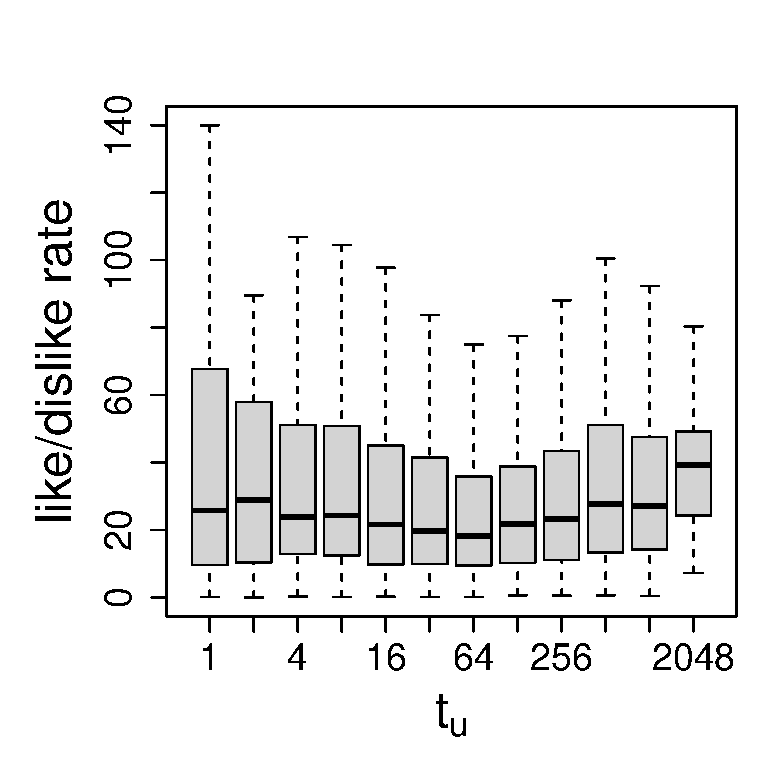
\includegraphics[width=2.5in]{figures/youtube_like_dislike_rate.eps}
& 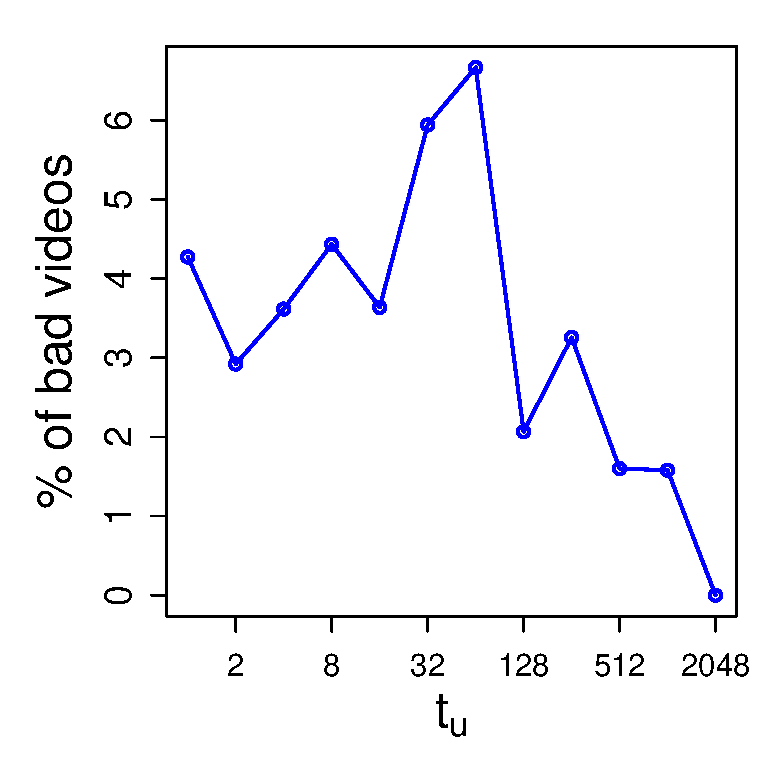
\includegraphics[width=2.5in]{figures/youtube_bad_rate.eps} \\
(a) Average likes/dislike rate & (b) Bad video rate
\end{tabular}
\caption{The quality of videos as a function of decay time $t_u$. \emph{Like/dislike rate} is the number of likes divided by the number of dislikes. \emph{Bad videos} are those with the number of dislikes greater than half of the number of likes. There are in total 83 out of 2304 ``bad'' videos by our definition.}
\end{figure}

Sampling videos with different $t_u$ values suggests a further
way to break the YouTube videos in our set into categories.
We find that the most persistent videos are mostly music videos,
again underscoring the increasing appearance of art-related
topics in this class.
On the other hand, many home-recorded
video clips have very small value of $t_u$; as seen in Figure
\ref{fig:tu_tweet_rt}, content that fades away quickly might not have
lasting value, but in general is more viral. 
% I'm not sure I follow this; I'd either expand on it or omit. --Jon
% As suggested in
% \cite{Berger:10,Hansen:11}, viral content also tends to carry more
% positive sentiments - which can be the reason why people like more
% these amateur video clips.

\begin{figure}[htb!]
\centering
\epsfig{figure=figures/youtube_comment_view.eps, width=5in}
%\vspace{-0.1in}
\caption{Average number of views and comments as a funtion of $t_u$}
\label{fig:youtube_comment_view}
\end{figure}

Finally, in Figure \ref{fig:youtube_comment_view}, we consider the
number of views and comments on the videos in our set.
We find an increase in views and comments particularly for 
very large values of $t_u$, in a way that is more extreme
than the variation in the number of tweets from 
Figure \ref{fig:tu_tweet_rt}, and that also forms an intriguing
contrast with the trend in the number of RTs from that figure.
Understanding how persistence translates into these secondary
popularity measures such as view count is an interesting question.

%\begin{figure}
%\caption{Comparing likes and dislikes of YouTube videos. \emph{Bad videos} are defined as videos with the number of dislikes greater than half of the number of likes. There are 83 out of 2304 videos are ``bad'' by our definition.}
%\label{fig:youtubelike}
%\centering
%\epsfig{figure=fig/youtube_like_dislike.eps, width=5in}
%\end{figure}

%Regarding to our previous concerns that the long-lasting URLs can be spamy, it does not seem to be the case, at least for YouTube videos: the long-lasting ones are not disliked more than liked comparing to the short-lived ones. In fact, the long-lasting ones have a slightly higher likes/dislikes ration than the short-lived ones, on average.

\section{Conclusion}
In this chapter, we explore the relationship between content and the temporal dynamics of information in the context of TWitter. In particular, we find that using the textual features extracted from the content, we can predict the persistence of information with high accuracy. Second, we employ different text analysiss techniques to understand the nature of content that contributes to persistence. We examin and compare the fleeting and lasting content on three aspects, including the psychologuistic characteristics, trending words, and latent topics distribution. We find that the persistent information is more related to content with long-term value, such as positive emotions, life, family, and art. On the other hand, the rapidly-fading content contains
 mostly time-critical information that carries relatively more negative
sentiments, demanding more cognitive effort, or is associated with
quick action.

By restricting our scope of study to the time series of bit.ly URLs mentioned on Twitter, our findings can be limited to the types of social media and the dynamics of information they support. An interesting direction for future work could be studying the content and temporal patterns of information across systems. One possibility is to use the transcribed content of TV, radio, together with materials from online social madia. Also, since we only predicted the persistence of content for two extreme cases, it would be interesting to further investigate the connection between content and persistence as a continuous variable.


\chapter{Network structure and the spread of disengagement}
\label{chap:network}

%\section{Negative influence}

There has been significant focus on the dynamics of propagation in social networks, especially, with the local and global structure involved\cite{Newman:2002,Dodds:2005,Bakshy-2011,Leskovec:2007,Backstrom:2006,Romero-2011,Nowell-2008,Gruhl-2004}. In many cases, such as the decision to become a member or use a product, the story does not end at
adoption.  Instead, the user may decide at any point to cease using
the product, or to depart the community.  It is not clear that a
decision of this type, to ``reverse'' a prior socially-mediated
decision to adopt, will follow the same dynamics as the original
decision to adopt.  In this paper, we study this question in the
context of arrivals and departures within online social networks.

A natural place to look for models of arrivals and departures is the
existing literature on the spread of infectious physical disease.
These models often include a recovery component\cite{Newman:2002,
  Dodds:2005}, which is akin to a reversal of the decision to become
infected.  Typically, however, this component assumes that an infected
user recovers based on properties of the immune system, without
reference to any social process.  In our case, we are motivated by the
metaphor of a user at a party with friends.  The user is more likely
to attend upon discovering that some number of friends will also
attend.  If some or all of the friends then opt to depart, whether for
a new party or to curl up with a good book, then the original user is
much more likely to follow suit.  Hence, we anticipate that social
forces play a significant role in both arrivals and departures.

We begin to address this question with a basic study of the temporal
correlation of arrivals and departures, and show that both processes
introduce significant correlation among friends; in fact, we show that time intervals between
the departure of friends are more tightly distributed than the
equivalent distribution of gaps between arrival of friends.

In this sense, we might consider arrival as the propagation of a
``join'' virus, and departure as simply the propagation of a new
virus, in this case representing the decision to cease usage.
However, this formulation is at odds with our conception of the
underlying process.  It is plausible that seeing one friend join a
social network, then two, then three, might impel a user to join, as
we see in prior work~\cite{Backstrom:2006}.  However, once a user has two
hundred friends, will the departure of one, then two, then three friends 
have a qualitatively different impact on the user's likelihood to
depart?  Perhaps like the decision to join, the decision to depart
depends more on the number of active friends than the number of
inactive friends.  Or perhaps departure is a fundamentally different
decision that depends on an assessment of the pulse of the
neighborhood, captured more accurately by the fraction of friends who
remain active.

We study this question in the context of a large social network, and
argue that in fact a hybrid of these models provides the most accurate
characterization.  While number of active neighbors is known to be a
strong predictor of joining a group, for users with twenty or more
friends, overall neighborhood activity, measured by the fraction of
friends who remain active, is by far the best predictor of likelihood
to depart.  Surprisingly, this likelihood is linear in the fraction of
active friends throughout almost its entire range, and the linear form
is identical in both slope and intercept for several different buckets
of neighborhood size.  Raw counts of inactive friends have low
predictive power, and raw counts of active friends, while stronger,
remain weak compared to the overall fraction of active friends.  On
the other hand, for users with fewer than twenty friends, the actual
count of active friends remains a strong predictor of likelihood to
depart. From these findings we reach a picture that users with few
friends rely heavily on their continued presence, while users with
more friends are pushed one unit closer to departure by each
successive fraction of existing friends observed to depart.

From this emerging local picture of behavior, we may then ask how
arrival and departure dynamics interact with the global structure of
the graph.  In particular, we seek to understand where departures
happen in the graph.  It is possible, for example, that departures
tend to occur as high-status users in the core of the graph choose to
depart in search of the next big thing.  Alternately, it is possible
that departure happens at the ``fringes'' of the graph, and then
spreads inwards from there.  We study this problem by computing the
density and conductance of the subgraphs of active and inactive users
through time, and comparing these results to thought experiments in
which each node decides independently whether to remain active.  These
experiments allow us to conclude that a core of active nodes remains
at much higher internal density than the set of inactive nodes. We
also compare the densities observed against the expected density and
conductance under a planted degree constraint model.  The results
suggest that although the inactive set of nodes densifies, its densification is
not just a consequence of the degree distribution, but really a
consequence of well-connected cluster of nodes from the fringes
departing.  We are led to believe that departures happen from the
fringes and heavily influence their immediate neighborhoods, while
an internal dense core of active nodes survives.

\section{Data}

In this chapter, we study the structure properties in relation to the arrival and departure of users, using a snapshot
of the DBLP co-authorship graph and a well-known social network.  The DBLP snapshot
that we consider contains 1072718 nodes and 1839605 edges, for each author we store his/her co-authors
and the year of the last publication. Furthermore for each author to author edge we also
store the year of the first publication. in the rest of the paper we will refer to
it as DBLP. The network we study contains millions of
users and over a billion edges.  For each user, we have the timestamp
of signup and last login, and for each edge, we have the timestamp of
edge creation. In the rest of the paper we will refer to this network as SN.  

To study the pattern of user arrivals and departures, we first
describe each user at each timestamp as either active or inactive,
based on his most recent activity time. Given a snapshot of the SN network
at time $t$, we consider a user \emph{inactive} if his last login time
is earlier than two months prior to $t$, and consider a user
\emph{active} otherwise. Given a snapshot of the DBLP network
at time $t$, we consider a user \emph{inactive} if he/she has not published any 
paper in the earlier than five year prior to $t$, and consider a user
\emph{active} otherwise. Note that our results do not depend on the time frame that we used. In fact, they hold for two quite different networks and time frames.

\section{Arrival and departure correlation among friends}
In this section, we study the temporal patterns of arrivals and
departures, for both local dynamics and global trends.  We wish to understand whether users typically arrive
and/or depart together in social networks.  However, we cannot
directly compare gaps between arrivals and departures of friends, as
networks are not stationary---consider for example the case of a
network that grows very rapidly during a brief period, resulting in a
flurry of temporally-proximate arrivals, leading to a mistaken
conclusion that arrivals tend to be tightly clustered in time.

We must therefore normalize in some way against global rates of
arrival and departure, which we do by the following technique. Given a snapshot of the network at time $t$, we
consider two samples of user-pairs, one in which the pair of users are
friends, and another in which the pair of users is chosen uniformly
from all possible pairs\footnote{Note that although technically, it is possible for a random pair to be a pair of friends, 
%as we only sample 1M among the total tens of billions of possible pairs, 
given the service policy that each user has a rather small upperbound for the number of friends, the chance of a random pair being friends is negligible.}.  We then consider the distribution of the gap in arrival time between pairs in the two cases.  Differences in these
distributions will then highlight temporal correlation of arrivals of
friends compared to strangers.

To study departures, we adopt the same technique.  We consider only
inactive users, and generate again a set of
pairs of friends, and another set of pairs chosen uniformly at random.
In this section, we fix $t$  then define the last login time of inactive users as their departure time. We pick 1M pairs for each of these four sample groups, and shows the
Cumulative Distribution Function (CDF) for these distributions in Figure~\ref{fig:time_gap_cdf}.

\begin{figure}[h]
\centering
%\vspace{-8pt}
\subfigure[SN]{\label{fig:orkut_time_gap_cdf}\includegraphics[width=0.40\textwidth]{figures/arrival_and_departure_time_gap_cdf.eps}}       \hspace{0.05\textwidth}            
\subfigure[Dblp]{\label{fig:dblp_time_gap_cdf}\includegraphics[width=0.40\textwidth]{figures/dblp_arrival_and_departure_time_gap_cdf.eps}}
\caption{\small The CDF curve for the difference in arrival and departure
  time between friends and random pairs of users.}
 \label{fig:time_gap_cdf}
%\vspace{-3pt}
\end{figure}

The CDF for both arrivals and departures of friends lies significantly
above the CDF for random pairs, indicating that friends both arrive
and depart together, in comparison to the control group of random
pairs.  As the figure shows, in the case of SN $43\%$ of random pairs depart within 200
days of one another, while $61\%$ of friends depart within the same
period, a large relative increase of $41\%$. We find similar pattern in the time interval of arrival - only $31\%$ of random pairs arrive within 200 days, but $45\%$ of friends arrive within the same period. This observation is even more evident in Dblp where the lines are clearly apart.

To quantify the differences, we plot in
Figure~\ref{fig:friend_random_cdf_gap} the distribution of absolute
difference in the CDF values at each time, for arrivals and
departures(at least in SN).  The correlation of departures is seen to be stronger than
the correlation of arrivals, although the two gaps peak around roughly
the same value.


%% A possible explanation for this observation is that some of the
%% friendship only formed online - after two friends both sign up to the
%% service, thus the impact of friendship of this kind is weak, or does
%% not exist before a user arrives. Evidence for this explanation can be
%% seen in Figure~\ref{fig:friend_signup}.

%%TODO(shaomei): add description, more discussion 

\begin{figure}[h]
\centering
\small
%\vspace{-8pt}
\subfigure[SN]{\label{fig:orkut_friend_random_cdf_gap}\includegraphics[width=0.40\textwidth]{figures/friend_random_cdf_gap.eps}}     \hspace{0.05\textwidth}              
\subfigure[Dblp]{\label{fig:dblp_friend_random_cdf_gap}\includegraphics[width=0.40\textwidth]{figures/dblp_friend_random_cdf_gap.eps}}
%\epsfig{file=}
\caption{\small Gap between CDF curves.}
\label{fig:friend_random_cdf_gap}
%\vspace{-3pt}
\end{figure}

We also consider the eventual set of friends acquired by a user at the snapshot time $t$, and
ask whether those friends join before or after the user.  First, in contrast to the observations in previous research\cite{Backstrom:2006}, the number of friends who already signed up seem to have a ``diminishing effect'' only on the case of the co-authorship graph and not of SN. In Figure~\ref{fig:friend_signup_count}, we see that in SN as the number of adopted friends increases, the probability of a user signup increases, but rather linearly, throughout almost the entire range x-axis. On the other hand, the expected
fraction of friend pairs joining before the user will always be 0.5, as the friend network is undirected and each edge contributes one pair in
which $a$ joins before $b$, and the opposite pair in which the reverse
happens.  Thus, for regular graphs (of constant degree), the mean of
the distribution of fraction of friends already signed up will be at
0.5.  The results are shown in Figure~\ref{fig:friend_signup}.  True
social networks are of course non-regular, and while the distribution
of plot (Figure~\ref{fig:friend_signup_fraction}) appears largely symmetrical, there are some outliers.  In particular, both in SN there are more than 20 times as many users users for whom, at
signup, 100\% of their friends have already signed up, compared to
users for whom 0\% of their eventual friends have already signed up. These can be explained by many low-degree nodes who are attracted to the network by a friendship invitation but never really engage in the network afterwards. In Dblp the situation is a bit different, this is probably explainable by the fact that several papers are written by community of student that after the master or the PhD do not publish any more. Overall, we think that there is certain network effect towards the arrival of users, however, this effect is quite weak in the formation of the network, and may not be enough to actively engage users after they sign up.

%These are explained by high-degree nodes who tend to arrive relatively
%early in the system, inviting many friends who join but never become
%aggressive about inviting additional friends.

%%TODO(shaomei): plot the friend_signup_count in CDF.

\begin{figure}[ht]
\centering
\small
%\vspace{-8pt}
\subfigure[Count(SN)]{\label{fig:friend_signup_count}\includegraphics[width=0.4\textwidth]{figures/friend_signup_count_dist.eps}}       \hspace{0.05\textwidth}          
\subfigure[Fraction(SN)]{\label{fig:friend_signup_fraction}\includegraphics[width=0.4\textwidth]{figures/friend_signup_frac_dist.eps}}\\
%\vspace{-8pt}
\subfigure[Count(Dblp)]{\label{fig:dblp_friend_signup_count}\includegraphics[width=0.4\textwidth]{figures/dblp_friend_signup_count_dist.eps}}       \hspace{0.05\textwidth}   
\subfigure[Fraction(Dblp)]{\label{fig:dblp_friend_signup_fraction}\includegraphics[width=0.4\textwidth]{figures/dblp_friend_signup_frac_dist.eps}}
\caption{\small Count and Fraction of friends already signed-up when user
  signs up.}
\label{fig:friend_signup}
%\vspace{-3pt}
\end{figure}

Our conclusion from this set of graphs is that friends tend to arrive
and depart together, but departures are more tightly clustered than
arrivals.  This observation relates only to individual friends, while
we expect that the effects are better understood in terms of the
entire ``neighborhood'' of friends in the graph.

Arrivals are difficult to study in this model, as the nature of the
neighborhood is largely unknown to a new user until after the decision
to join.  Other authors consider the related problem of joining a
particular group as the adoption of an innovation within the substrate
of an existing social network.  For example, \cite{Backstrom:2006}
consider joining an interest group within the LiveJournal network.  We
may therefore employ our longitudinal data to flesh out the picture
given by this earlier, by looking more closely at the impact of the
neighborhood structure on departure.  Subsequently, we then relate the
results back to known literature on adoption of innovations around
group membership, to compare what is known about arrivals and
departures.

\section{Effect of local neighborhoods}

\begin{comment}
To test the correlation in departure among friends, we begin by simply comparing the difference in last login times between friends and random pairs of users. 
%Here the departure time is defined as the last login time, for users who are inactive. 
We randomly sample 8 million friendship edges and 8 million random pairs of inactive nodes, calculate the gap $\delta_t$ (in days) for each pair, and plot the CDF curves in Figure~\ref{fig:inactive_timing_cdf}. 

\begin{figure}[h]
\centering
\includegraphics[height=60mm,width=60mm]{figures/departure_time_gap_cdf.eps}
%\epsfig{file=}
\caption{The CDF curve for the difference in last login times between inactive users who are friends and random pairs of inactive users.}
\label{fig:inactive_timing_cdf}
\end{figure}

In Figure~\ref{fig:inactive_timing_cdf}, the curve for friends is
constantly above the curve for random pairs, showing that someone is
much more likely to login if his/her friends are logging in
frequently. For example, when $\delta_t=180$, the gap between the two
CDF curves is around $0.15$; we see around half of the friendship
edges have both nodes logged in within 180 days, and only $35\%$ of
the random pairs logged in within this interval.  
\end{comment}

As shown in previous section (Figure~\ref{fig:time_gap_cdf}), friends are more likely than strangers to have logged in within around half year of
one another.  This dramatic difference causes us next to look beyond
single-edge correlations to properties of the entire neighborhood of a
node.

\subsection{Dependence on local properties}
The correlation in the timing of last login among friends suggests the effect of friends' inactivity on the decrease of activities on an individual. To better understand how a user's departure is influenced by his local community, in this section, we look at the probability of a user's departure in relation to the following four properties related to the user's neighborhood.

%\vspace{-5pt}
\begin{itemize}\addtolength{\itemsep}{-.35\baselineskip} 
\item number of active friends;
\vspace{-5pt}
\item fraction of active friends;
\vspace{-5pt}
\item number of inactive friends;
\vspace{-5pt}
\item number of inactive friends who left in the past 6 months;
\end{itemize}
\vspace{-5pt}

\begin{figure*}[htb]
\centering
%\vspace{-8pt}
\subfigure[]{\label{fig:orkut_p_k_active_curve}\includegraphics[width=0.4\textwidth]{figures/p_k_active_curves.eps}} \hspace{0.05\textwidth}
\subfigure[]{\label{fig:orkut_p_k_curve}\includegraphics[width=0.4\textwidth]{figures/p_k_curves.eps}}\hspace{0.05\textwidth} \\
\subfigure[]{\label{fig:dblp_p_k_active_curve}\includegraphics[width=0.4\textwidth]{figures/dblp_p_k_active_curves.eps}} 
\hspace{0.05\textwidth}
%\vspace{-8pt}
\subfigure[]{\label{fig:dblp_p_k_curve}\includegraphics[width=0.4\textwidth]{figures/dblp_p_k_curves.eps}}\hspace{0.05\textwidth} \\
\subfigure[]{\label{fig:orkut_p_f_active_curve}\includegraphics[width=0.4\textwidth]{figures/p_f_active_curves.eps}}
\hspace{0.05\textwidth}
\subfigure[]{\label{fig:orkut_p_r_curve}\includegraphics[width=0.4\textwidth]{figures/p_r_curves.eps}}
\caption{\small Probability of departure as function of different local properties. Where (a) is $p$ as f(active friend count) in SN, (b) is $p$ as f(inactive friend count) in SN, (c) is $p$ as f(active friend count) in Dblp, (d) is $p$ as f(inactive friend count) in Dblp, (e) is $p$ as f(active friend fraction) in SN and (f) is $p$ as f(inactive friends who left in the past 6 months) in SN.}
\label{fig:p_plots}
%\vspace{-3pt}
\end{figure*}

To study how the probability of a user becoming inactive depends on the number of friends who are active, we use a similar method as in \cite{Backstrom:2006}: we first take two snapshots $(t_0, t_1)$ of the network, three months apart in SN and three years apart in Dblp; we then find all pairs $(u,k)$ such that $u$ is active at the time of first snapshot $t_0$, and has $k$ friends who are also active at $t_0$; $p(k)$ is calculated as the fraction of such pairs $(u,k)$ for a given $k$ such that $u$ had left the network at the time of second snapshot $t_1$. In other words, $p(k)$ is the fraction of active users who left the network in the next three months, given that $k$ friends are active at the first snapshot time. Figure~\ref{fig:orkut_p_k_active_curve} and Figure~\ref{fig:dblp_p_k_active_curve} shows the curves of $p(k)$ at three different sample points of $t_0$. In a similar way, we can fix $f$ as the fraction of friends who are active at time $t_0$, and calculate the probability $p(f)$ of an active user leaving the network as function of $f$ (see Figure~\ref{fig:orkut_p_f_active_curve}). Note that for this figure and all the following figures involving the fraction of active/inactive friends, we exclude all the nodes with no friends in SN, which are around $10\%$ of all active users as of 2011/1/1, and among those users, $35\%$ of them left within three months. 

Not surprisingly, Figure~\ref{fig:orkut_p_k_active_curve}, Figure~\ref{fig:dblp_p_k_active_curve} and Figure~\ref{fig:orkut_p_f_active_curve} show that as more and more friends stay active, a user is less and less likely to be inactive. The curve of $p(k)$ (see Figure~\ref{fig:orkut_p_k_active_curve}) also matches very well with what has been seen in other domains \cite{Backstrom:2006}, exhibiting the ``diminishing returns'' property - as the number of active friends $k$ increases, the probability of departure continues to decline, but more and more slowly, eventually converging to a constant for very large values of $k$. This observation indicates that the marginal gain of having each additional active friend is quite significant for users with a small number of active friends, but rather negligible when a user has already more than 50 active friends. In contrast, in Figure~\ref{fig:orkut_p_f_active_curve}, we do not see such a ``diminishing returns'' trend, but a steeper, and almost constant rate of decrease in the probability of departure throughout the course when the fraction of active friends increases. This is an interesting observation that has not been previously seen (specifically in various positive influence studies). 
%This suggests that the fraction of active friends has a stronger effect on the probability of departure than the count of active friends. 
% I commented this last sentence since currently theory is only for number, and also in some other plots we see number also as being quite important. So perhaps better not to make this categorical statement - Atish.

To see how the inactivity of the neighborhood influences the departure of a user, we also plot the probability of departure as a function of number of inactive friends, in Figure~\ref{fig:orkut_p_k_curve} and Figure~\ref{fig:dblp_p_k_curve}. The curves in Figure~\ref{fig:orkut_p_k_curve} and Figure~\ref{fig:dblp_p_k_curve} show an interesting trend of decreasing slope through time: while the probability of a user departing increases with the growth in the number of inactive friends in initially, it becomes more and more insensitive to the value of $k$ in the later curves. This phenomenon is quite intriguing to us: if the departure of friends do have a clear effect on the departure of the user, as shown in the earlier curves, why is this effect diminished so much in the latest years? To answer this question, we note that we are counting the number of inactive friends as prior to the time of each snapshot, but many of them could have been inactive for a long time thus could hardly influence the user's experience in the network at the snapshot time. Figure \ref{fig:orkut_p_r_curve} confirms this idea, showing that the curves we see in Figure~\ref{fig:orkut_p_k_curve} are somewhat misleading -  in general, the probability of user's departure constantly grows with the number of friends $r$ who \emph{recently} became inactive (when $r$ is not too small). 
 
%Figure~\ref{fig:p_k_curve} shows the curves of $p(k)$ at three different sample points of $t_0$. The results surprisingly contrasts our expectation in two ways. First, there is an initial drop in the probability of departure along with the increase of $k$ - especially, when $k$ grow from $0$ to $1$, the probability of a user leaving drops for over/about $50\%$. Second, the remainder of each curve shows small (2009,2010) or no (2011) increase in $p(k)$ as $k$ grows. It seems that through time, the departure of a user is more and more insensitive to the number of friends who have already left. 

%A possible explanation for the first phenomenon is that the user with $0$ departed friends are those who either never engaged in the network, or make decisions independently of their friends' activities, thus are less attached to the network and are more likely to leave; and for those who have engaged in the network, the departure of one or two friends is hardly noticeable, thus the small non-zero value of $k$ is associated with a low departure rate.

%The second phenomenon is more intriguing to us: if the departure of friends do have an positive effect on the departure of the user, as shown in the earlier curve, why does $p(k)$ stays flat as $k$ increases, in the year of 2011? To answer this question, we note that we are counting the number of inactive friends as prior to the time of each snapshot, but many of them could have been inactive for a long time thus could hardly influence the user's experience in the network at the snapshot time. Figure \ref{fig:p_r_curve} confirms this idea, showing that the curves we see in Figure~\ref{fig:p_k_curve} are somewhat misleading -  in general, the probability of user departure constantly grows with the number of friends $r$ who \emph{recently} became inactive (when $r$ is not too small).   


%\begin{figure}[h]
%\centering
%\includegraphics[height=60mm,width=60mm]{fig/p_r_curves.eps}
%\caption{The probability $p$ of leaving the network in the next 3 months as a function of the number of friends $r$ left the network in the past 6 months prior to the snapshot time.}
%\label{fig:p_r_curve}
%\end{figure}


%Having found the dependence of the probability of user becoming inactive on the number of inactive friends, we now explore the relationship between a user's departure and the fraction of inactive friends in his neighborhood, as shown in Figure~\ref{fig:p_f_curve}. Similarly to what we have seen previously, after an initial drop, the probability of a user leaving the network increases as the percentage of inactive friends grows. However, the curves in Figure~\ref{fig:p_f_curve} exhibit a much steeper slope than previous ones, suggesting a stronger correlation between the probability of user departure and the fraction of friends who have departed. 

\subsection{Interaction between local properties}

The results of the previous section provide qualitative evidence that an individual's probability of departure is related to the activeness of his neighborhood. Intuitively, as more and more friends leave a social network, a user will start to feel desolated and will be more likely to leave as well. Our previous results also suggest that the fraction of friends who are active/inactive contributes to the overall atmosphere of the neighborhood, and that this matters more than the raw number of active/inactive friends. However, does that apply to all users? Do the highly connected users act differently than the more marginally connected ones? Can people really notice and act on the degeneration of their neighborhood, or will they stay as long as there are a few active friends, in spite of a large fraction of their friends having left? To address these issues, we compute the probability of user's departure in SN in relation to the interaction between local properties. Specifically, in Figure~\ref{fig:p_f_3_level}, we divide users into three groups based on their degrees, and plot the probability of departure as a function of the number/fraction of active friends, for each group separately. We note that for users with different levels of connectivity in the network, the curves of $p(f)$ (Figure~\ref{fig:p_f_3_level}) are qualitatively identical. This result demonstrates again that the fraction of friends who are active has a stronger effect on the probability of an individual's departure, regardless of the size of the user's neighborhood.
% Again I am not sure if we should omit or reword this last sentence - Atish

In addition, we aggregate users by the fraction of active/inactive friends, and look at how the probability of departure depends on the number of active/inactive friends for each group (see Figure~\ref{fig:p_k_3_level}). There are two things we note from Figure~\ref{fig:p_k_3_level}: First, for users with different fractions of inactive friends, there is a big gap between their probabilities of departure - for example, compared to users with less than $10\%$ friends left (blue line in Figure~\ref{fig:p_k_inactive_3_level}), users who have more than $50\%$ friends left (red line in Figure~\ref{fig:p_k_inactive_3_level}) are $10$ times more likely to leave as well. Second, once the user is in an inactive part of the neighborhood, the raw count of inactive friends has little effect in determining the probability of the user's departure (green line in Figure~\ref{fig:p_k_active_3_level}). Note that the blue line in Figure~\ref{fig:p_k_active_3_level} is very noisy because there are very few people in a highly obsolete neighborhood but still with a substantial amount of active friends. We still plot it just to be symmetric with Figure~\ref{fig:p_k_inactive_3_level}.

\begin{figure*}[htb!]
\centering
%\vspace{-8pt}
\subfigure[]{\label{fig:p_f_3_level}\includegraphics[width=0.4\textwidth]{figures/p_f_active_3_levels.eps}} \\
%\hspace{0.03\textwidth}   
\subfigure[]{\label{fig:p_k_active_3_level}\includegraphics[width=0.4\textwidth]{figures/p_k_active_3_levels.eps}} \\ %\hspace{0.03\textwidth}   
%\subfigure[$p(f)$ group by total number of friends.]{\label{fig:p_f_active_3_level}\includegraphics[width=0.35\textwidth]{fig/p_f_active_3_levels.eps}}\\
\subfigure[]{\label{fig:p_k_inactive_3_level}\includegraphics[width=0.4\textwidth]{figures/p_k_3_levels.eps}}
%\hspace{0.05\textwidth}               
%\subfigure[$p(f)$ group by total number friends.]{\label{fig:p_f_3_level}\includegraphics[width=0.35\textwidth]{fig/p_f_3_levels.eps}}
\caption{Probability of departure as function of local properties, at different levels of active/inactive friend fraction and friend count (snapshot taken at time $t=$2011/1/1). in SN}
\label{fig:p_k_3_level}
%\vspace{-5pt}
\end{figure*}

\subsection{Predict the departure of user}
Given a strong correlation between the probability of a user becoming inactive and the inactivity of his friends, the next question is, can we actually predict individuals's departures based on local properties? In this section, we explore the problem of modeling the departure of users using simple linear regression models and decision tree classifiers. In particular in this subsection we will focus exclusively on SN because we have a richer set of feature available.

To start, we formalize our problem as a binary classification task in which class 1 is defined as consisting of those users who were active as of Jan 1st, 2011 ($t_0$) and departed within two months after $t_0$, and class 0 is defined as consisting of those who stayed active for two months after $t_0$. We then randomly sample 500K positive examples and negative examples separately, from all the users who were active at $t$. Note that among all examples, there are $90\%$ negative and only $10\%$ positive examples; our sampling scheme provides a more balanced distribution of examples of both classes. 

We extract two sets of local features for each user:
\begin{itemize}
%\vspace{-8pt}

	\item Neighborhood features. The local structural properties of the user's direct neighborhood, including the number of friends who already departed, the number of friends who are active, the number of friends who departed recently (six months prior to $t_0$), and the fraction of friends who departed recently.
\vspace{-8pt}

	\item Activity features. The properties reflecting user's participation to activities in the network, including the number of contents he received, the number of contents he sent, and the number of status updates.
\end{itemize}

To predict the departure of users, we train a simple decision tree (REPTree) classifier on our examples. Table \ref{table:departure-performance} gives the performance of the classifier with different sets of features under 10-fold cross validation. 

\begin{table}[t]
%	\small
	\centering
	\caption{ \small Predict user departure with decision tree}
	\label{table:departure-performance}
	\begin{tabular}{c|c|c|c}
	\hline
	\emph{Feature} & \emph{Accuracy} & \emph{F1 pos} & \emph{ROC area}\\
	\hline
	Neighborhood & 0.694 & 0.694 & 0.755 \\
	\hline
	Activity & 0.730 & 0.735 & 0.801 \\
	\hline
	All & 0.755 & 0.761 & 0.833 \\
	\hline
	\end{tabular}
\end{table}

Table \ref{table:departure-performance} shows that relying on only local features of individuals, the simple decision tree classifier can predict the departure of user with high accuracy ($75\%$ with all features, as compared to $50\%$ for always predicting one class). This result demonstrates a strong connection between user's local properties and the propensity of departure. Moreover, comparing across 3 sets of features, we see that although the activity features are more powerful, neighborhood features can also provide rather accurate insights on the departure of users. 

The decision tree classifier demonstrates that local properties provide strong evidence to predict the departure of user. It also suggests that the activity features are more effective at predicting user departure. However, the decision trees we trained contain over a thousand nodes and thus is too complicated to illustrate how the local properties influence the probability of user departure. To better understand the effect of different features, we also fit the data with a logistic regression model that predicts the probability of departure. The model is constructed on 7 independent variable covering both neighborhood features and activity features, the results of the model is summarized in Table~\ref{table:logistic_regression_result}

\begin{table}[t]
\small
	\centering
%	\small
	\caption{\small Summary of logistic regression model on $p_{departure}$}
	\small
	\label{table:logistic_regression_result}
	\begin{tabular}{c|r|l}
	\hline
	\emph{Feature} & \emph{Coefficient} & \emph{$p$ value} \\
	\hline
	1/(number of active friends) & 0.0579 & $<2e-16$ ***\\
	\hline
	fraction of active friends & -1.5340 & $<2e-16$ ***\\
	\hline
	number of friends left recently & 0.0067 & $<2e-16$ ***\\
	\hline
	fraction of friends left recently & -0.0020 & 0.0737 . \\
	\hline
	number of contents received & -0.0012 & $<2e-16$ *** \\
	\hline
	number of contents sent & 0.0000 & $1.28e-06$ *** \\
	\hline
	number of status updates & -0.0017 & $<2e-16$ *** \\
	\hline
	\end{tabular}
	\normalsize
\end{table}

We evaluate the logistic regression model using 10-fold cross validation as well, and it only slightly under-performs the decision tree classifier, with the ROC area as 0.774. 

The results of the regression model nicely confirm the descriptive results we showed previously, and quantify the effect of different variables on the departure probability. In particular, from Table~\ref{table:logistic_regression_result}, we see that the existence of active friends and continued activities, both decrease a user's tendency to depart while the number of friend who departed recently contribute to this tendency. We also notice that although most of the activity variables and the neighborhood variables have very high significance (very low p-value) in the estimated model, each unit of the fraction of active friends has the most substantial effect on the probability of user departure.

%(TODO:(shaomei) Disucss more the results of logistic regression model)

\section{Structural trends in network topology}
\label{sec:global}

\begin{figure*}[htb!]
\centering
\subfigure[active(SN)]{\label{fig:orkut_edge_active}\includegraphics[width=0.30\textwidth]{figures/edges_active.eps}}                \hspace{0.02\textwidth} 
\subfigure[inactive(SN)]{\label{fig:orkut_edge_inactive}\includegraphics[width=0.30\textwidth]{figures/edges_inactive.eps}} \hspace{0.02\textwidth}
\subfigure[semi-active(SN)]{\label{fig:orkut_edge_semi_active}\includegraphics[width=0.30\textwidth]{figures/edges_semi_active.eps}}\\
\subfigure[active(Dblp)]{\label{fig:dblp_edge_active}\includegraphics[width=0.30\textwidth]{figures/dblp_edges_active.eps}}                 \hspace{0.02\textwidth}
\subfigure[inactive(Dblp)]{\label{fig:dblp_edge_inactive}\includegraphics[width=0.30\textwidth]{figures/dblp_edges_inactive.eps}} \hspace{0.02\textwidth}
\subfigure[semi-active(Dblp)]{\label{fig:dblp_edge_semi_active}\includegraphics[width=0.30\textwidth]{figures/dblp_edges_semi_active.eps}}
\caption{Distribution of edges, indicated by the ratio of actual number of edges over the expected number of edges (formed in random process).}
\label{fig:edges}
\end{figure*}

We explore the overall structural changes that occur in the network as a result of the departure of several users, as well as the steady arrival of new users. Topological changes have been studied in the context of new nodes arriving but here we pay specific attention to how the global structure changes as a result of the departure or decline of user activities based on their local neighborhoods. 

To get a sense of the how the structure of the network evolves over time, we
first study the distribution of edges among active and inactive
nodes. Specially, we look at the edges between active nodes (Figure~\ref{fig:orkut_edge_active} and Figure~\ref{fig:dblp_edge_active}), edges between
inactive nodes (Figure~\ref{fig:orkut_edge_inactive} and Figure~\ref{fig:dblp_edge_inactive}), and the edges across active and inactive nodes (Figure~\ref{fig:orkut_edge_semi_active} and Figure~\ref{fig:dblp_edge_semi_active}), and plot the
ratio between the actual number of edges over the expected value over time.
%

Here, the expected number of edges is computed based on the total number of edges, $|E|$, in the network and the number of nodes in each of the active and inactive sets. The expected number of edges of any type is the expected number of edges if the the total $|E|$ edges are placed between randomly chosen pairs of nodes.


%The plot for the number of active, inactive, and total number of nodes in the networks is shown in Figure~\ref{fig:nodes}. The corresponding plot for the total number of active edges, inactive edges, and semi-active edges (one end node active and other inactive) are shown in Figure~\ref{fig:edges}. The corresponding expected numbers, as measured based on the overall number of edges and number of nodes, is also shown in the same figure. 

%\begin{figure}[h]
%\centering
%\includegraphics[width = 1.0\linewidth]{fig/nodes.eps}
%\caption{Nodes}
%\label{fig:nodes}
%\end{figure}


%\begin{figure}[h]
%\centering
%\includegraphics[height=60mm,width=60mm]{fig/edges.eps}
%\caption{Edges}
%\label{fig:edges}
%\end{figure}

To understand the overall structure among the sets of active and inactive nodes, we study the density and conductance of these two sub-networks in the rest of this section.

Figure~\ref{fig:density} and plots the overall density of the active (\ref{fig:density_active} and \ref{fig:dblp_density_active}) and inactive (\ref{fig:density_inactive} and \ref{fig:dblp_density_inactive}) set of nodes, as a function of time. For comparison, we also plot the {\em expected} densities of the respective sets, as determined by the number of active and inactive nodes and edges and the degree distributions. 

We here define density of a set of nodes(or average induced degree) as the number of edges between them divided by the number of nodes; i.e. for a set of nodes $S$, $density(S) = \frac{|E(S, S)|}{|S|}$ (here $E(S, S)$ contains all edges $(u, v)$ such that $u, v\in S$). Therefore, the density of set $S$ is half of the average induced degree of the set of nodes in $S$. In order to compare the the density we observe for the set of active nodes and the set of inactive nodes, we define an {\em expected} density for each of these components. The expected density of the inactive set of nodes could be computed simply as the density of the entire graph times the fraction of inactive nodes. 

However, we even use a stronger baseline to see if the trends we observe are a result of a trend more than just that of degrees. Therefore, we compute expected density subject to the overall degree constraints on active and inactive nodes as follows. 

Consider each edge as occupying two slots (end points), each slot being in either $S_a$ (the active set of nodes), or $S_i$ (the inactive set of nodes); therefore $S_a\cup S_i = V(G)$. Let the fraction of all these slots that are in $S_i$ be $P_i$ (which is the number of edges going across the active and inactive component plus twice the number of edges in the inactive component); therefore the number of such slots occupied in $S_a$ is $P_a = (1-P_i)$. Suppose that all the $|E|$ edges were randomly placed in two slots each, with probabilities determined such that in expectation we respect $P_i$ and $P_a$, then we consider the induced density of this process as the expected density (for respective components). Notice that this is a more stringent baseline for our comparison. Therefore, an edge is contained in the inactive component with probability $P_i^2$ and so the expected density of the inactive set is $(|E|P_i^2)/|S_i|$. Similarly the expected density of the active component can be computed. 

\begin{figure}[htb!]
\centering
%\small
\subfigure[active]{\label{fig:density_active}\includegraphics[width=0.40\textwidth]{figures/density_active.eps}}           \hspace{0.03\textwidth}     
\subfigure[inactive]{\label{fig:density_inactive}\includegraphics[width=0.40\textwidth]{figures/density_inactive.eps}}\\
\vspace{-5pt}
\subfigure[active]{\label{fig:dblp_density_active}\includegraphics[width=0.40\textwidth]{figures/dblp_density_active.eps}}     \hspace{0.03\textwidth}           
\subfigure[inactive]{\label{fig:dblp_density_inactive}\includegraphics[width=0.40\textwidth]{figures/dblp_density_inactive.eps}}
\caption{Density of the active and inactive subnetworks}
\label{fig:density}
\end{figure}

%\begin{figure}[h]
%\centering
%\includegraphics[height=60mm,width=60mm]{fig/density.eps}
%\caption{Density}
%\label{fig:density}
%\end{figure}

The plots on these densities in Figure~\ref{fig:density} shows that the density
of the active set $density(S_a)$ increases rapidly with increase in
time. Comparing this with the plot on distribution of edges in
Figures~\ref{fig:edges}, we see that as the number of inactive nodes starts
increasing, the number of edges in the active set, and correspondingly its
density, becomes much higher than the density of the inactive set of nodes. We
notice that the density of the active set is only marginally higher than its
expected density. However, for inactive nodes, the density is significantly
higher than the expected density, even conditioned on the degree
distribution. This is only explainable by the fact that the decision to depart
is correlated across edges, as supported by our local analysis; the nodes that
are departing are still probably at the periphery of the network (since the
inactive set has much lower density than the active set), but these inactive
nodes continue to be internally well-connected because of a higher-than-expected
density. This strengthens the evidence from previous sections that a node's
likelihood to become inactive is influenced by the extent of neighboring
inactivity.

After learning about the connectedness of the active/inactive subnetwork separately, we now switch our gear to look at the connection of each subnetwork to the rest of social graph. We use conductance to measure the amount of possible connections between different sets of nodes in a network. 

\begin{figure}[htb!]
\centering
\subfigure[SN]{\label{fig:orkut_conductance}\includegraphics[width=0.40\textwidth]{figures/conductance.eps}}                \hspace{0.03\textwidth}
\subfigure[Dblp]{\label{fig:dblp_conductance}\includegraphics[width=0.40\textwidth]{figures/dblp_conductance.eps}}
\caption{Conductance of the active and inactive sets}
\label{fig:conductance}
\end{figure}

Conductance of a set of nodes $S$, $\phi(s)$ is measured as $\phi(S) = \frac{|E(S, V(G)\S)|}{|E(S)|}$. Here $E(S, V(G)\S)$ contains all edges $(u, v)$ such that $u\in S, v\notin S$, and $|E(S)| = 2|E(S, S)| + |E(S, V(G)\S)|$. So notice that conductance is always less than $1$, and any set with more than half its edges going across to the complement set has a conductance of more than $\frac{1}{3}$. We again measure the conductance of sets $S_a$ and $S_i$ through time and compare with their expected conductances (see Figure~\ref{fig:conductance}). The computation of expected conductance is also performed in a similar manner to as described previously for expected density. 

We see a similar trend in conductance in Figure~\ref{fig:conductance} as seen for densities. The conductance of the active set of nodes $S_a$, $\phi(S_a)$ remains somewhat less than the conductance expected for this set. This suggests that there are somewhat fewer edges going across from $S_a$ to the inactive set $S_i$ and far more edges within $S_a$ itself, than would be expected. The conductance plots for the set of inactive nodes however is again more contrasting. $\phi(S_i)$ remains far lower than the expected conductance. Nodes that are becoming inactive continue to have many more edges within, than one would expect. This clearly suggests that the inactive set of nodes are influencing neighbors to inactivity. Yet again, the absolute conductance value still suggests that nodes at the periphery of the network are more susceptible to becoming inactive. 

The takeaway from these plots are two fold. Firstly, of course, these trends
corroborate our findings from the previous sections suggesting that there is a
strong influence of inactivity on its neighborhood and that nodes are much more
likely to depart from the network if they are surrounded by inactive
nodes. However, these plots on global measures such as density and conductance
also suggest a picture of the evolving network. With the active set's density
being much higher than the inactive, and the inactive set showing higher than
expected density and lower than average conductance, we are led to believe that
nodes in the {\em core} of the network are much more likely to survive, while
nodes at the periphery are more susceptible to departure.

\section{Conclusion}
In this chapter, we have studied the dynamics of user departure from
online social networks, from the perspectives of local and global network structure. 
We considered the influence of local
neighborhoods on the behavior of nodes as well as studied global
changes in the network topology. At the local level, we studied
individuals and the dynamics in their local neighborhood, measured the
probability of user arrival and departure in relation to the
activity of their friends. Our findings are three fold: first, there
is a strong clustered effect in the timing of departure among friends
while this is not as visible in arrivals; second, although both
numbers and fractions of neighborhood (in)activity are correlated to
the probability of the individual's departure, the fraction of
inactive friends has arguably the strongest effect on the departure
probability, providing an interesting complement to literature on arrivals which
shows number of active friends as the most predictive of these
measures; third, once a significant fraction of friends depart, the
overall connectivity of individuals in the entire network does not
save the user from leaving the network. At the global level, we looked
at the trend of network topological properties over the past few
years, showing that as the network evolves, users at the peripheral
region of the network are more likely to depart in groups; yet an internal core
of the network survives and densifies over time. 

%, and may influence their neighborhood communities towards inactivity.
% 
%% It appears that the spread and influence of inactivity is slowly resulting in
%% the network peeling away from outside; however, the central core that is dense
%% and has low conductance (i.e. tightly knit within and sparsely connected
%% outside), is far more resilient to spreading inactivity. 
%% Perhaps peripheral nodes are more easily lured away from the network by a
%% combination of external forces and neighboring inactivity. At the other end, the
%% very well-connected central active set seems to survive and densify through
%% time, despite widespread departure of nodes.





%\part{Answer social science questions with social media data}

\begin{comment}
Information diffusion is a long term intersting problem in social science. Problems and small lit-review.


Online social media data provide us for the first time a more or less complete corpus to examine these social phenomenons in details. 


To handle data at this scale, we apply mixed methods and develop new tools (such as MR). 

By finding pattern in these large-scale dataset, we shed light on some long standing social science questions. 

Need to bear in mind that what we have found might be characteristics for social media, and might not be general truth in the offline environment. 

ZZZZZ: future work, compare results with other social media or offline data.


A better understanding of diffusion dynamics can contribute to some interesting long-term social science questions, such as the pattern of communications, diffusion of innovation, unfolding of social movements. Today��s user behavior data in social media can help us examine and possibly answer these questions quantitatively at a very large scale.

\chapter{Lasswell's Maxim}

\chapter{Two-step flow}

\chapter{Social movement}


\part{ZZZZZ: Previous structure...possibly move to intro}
\chapter{the interaction between people and information}

In~\cite{Wu-Twitter-2011}, we studied the production, flow, and consumption of information in Twitter. As suggested in previous research in public communications, we classified users into 5 categories (celebrities, bloggers, mass media, organizations, and others) and found a striking concentration of attention on a small number of ``elite'' users on Twitter, as well as a significant homophily within categories. We also applied the classical ``two-step flow'' theory of communications in the context of social media sites such as Twitter. Our results confirmed that there are a large number of intermediary users who actively filter and disseminate information from media to the masses, and the composition of intermediaries is highly diverse. We also examined the lifespan and content of URLs broadcasted by different categories of users. We found that although content picked up by bloggers tends to stimulate a more persistent interest, the longevity of information is determined not by diffusion process, but by many different users independently rediscovering the same content.




\chapter{the role of content}
Following up our previous work, in~\cite{Wu-ICWSM-2011}, we studied the relationship between content and the temporal dynamics of information on Twitter, focusing on the persistence of information. Our results demonstrated a strong association between the content and the temporal dynamics of information. For example, rapidly-fading information contains significantly more words related to negative emotion, actions, and more complicated cognitive processes, whereas persistent information contains more words related to positive emotion, leisure, and lifestyle.

\chapter{Network effect and behavioral contagion}

\chapter{Diffusion without active dissemination}

Arrival and Departure Dynamics in Online Social Networks (submitted to the International Conference on Web Wide Web, 2012). 

In this paper, we compared the dynamics of user arrival and departure in online social networks. We showed although user disengagement has been considered less viral than engagement, there is a substantial network effect of the departure of friends on a user's tendency to leave a network. Taking into account such network effect, we are able to build machine learning models to predict the departure of users based on their local network properties.


\chapter{Social media in Arab Spring Movement}
    Joining social media data with real world events, we are able to study one of the most interesting (and also the most difficult) parts in media communication research (Lasswell's maxim): the effect of information. One of my ongoing projects is to study the role of social media in social movements, in order to understand how the propagation of information is leading or reflecting societal changes. We have collected a large number of tweets and twitter networks related to big social movements (i.e., Middle East Revolution, Occupy WallStreet Movement). Using effective algorithms for community detection, hub detection, trend detection, and opinion mining, we will be able to identify the informal structure of massive communication networks for social movements and study the diffusion of ideology and behaviors within and across organizational/geographical boundaries.

\section{Background}
ZZZZZ: Summary of Arab Spring movement, major event timeline.

ZZZZZ: We observed a sharp increase of the social media usage during the arab spring period\cite{IPTPS}.  Such increase is considered not an accident but a driving force of the social movement \cite{}.

However, there is a debate about the role of social media in the revolution.

Previous research in this domain:

%1. Gilad Lotan, Erhardt Graeff, Mike Ananny, Devin Gaffney, Ian Pearce, and danah boyd (2011). "The Revolutions Were Tweeted:Information Flows during the 2011 Tunisian and Egyptian Revolutions." International Journal of Communications 5, Feature 1375-1405. http://www.danah.org/papers/2011/IJOC.html

%2. Kate Starbird, and Leysia Palen, "(How) Will the Revolution be Retweeted? Information Diffusion and the 2011 Egyptian Uprising", CSCW 2012 http://www.cs.colorado.edu/~palen/StarbirdPalen_RevolutionRetweeted.pdf

% 3.Philip N. Howard, Aiden Duffy, Deen Freelon, Will Mari, and Marwa Mazaid, "Opening Closed Regimes. What Was the Role of Social Media During the Arab Srping?", Working paper  2011.1http://dl.dropbox.com/u/12947477/publications/2011_Howard-Duffy-Freelon-Hussain-Mari-Mazaid_pITPI.pdf

% 4. Sandra Gonzalez-Bailon, Javier Borge-Holthoefer, Alejandro Rivero, and Yamir Mareno, "The Dynamics of Protest Recruitment through an Online Network" , Nature, Scientific Reports, 2011/12/15 http://www.nature.com/srep/2011/111215/srep00197/pdf/srep00197.pdf

% There aren't (yet) many scholarly articles that examine the actual process of mobilization in the Arab Spring. I know of people working on them, but nothing published yet.

% That said, POMEPS had a review of the Egyptian revolution that discusses the important role of activists in mobilization (attachedhere.) Similarly, Marc Lynch's book "The Arab Uprising: The Unfinished Revolutions of the New Middle East" and James Gelvin's "The Arab Uprising: What Everyone Needs to Know" are two good books that *describe* how the processes unfolded and both of these texts discuss the role of Egyptian activists and their development since 2006. They are more for an educated but general audience, however, and none of them have claims about one factor being more important than the other, but they all discuss how central April 6, the Muslim Brotherhood, etc. were for mobilization in Egypt. If we want substantive support of the data, these could be useful.

% Similarly, there are many articles in online journals/magazines that also argue for the role of organized groups in Egypt. For example:
% Who is behind the Egyptian Revolt? http://www.thenation.com/blog/158159/whos-behind-egypts-revolt
% The Praxis of the Egyptian Revolution http://www.merip.org/mer/mer258/praxis-egyptian-revolution

Questions to answer:
\begin{enumerate}
\item Whether Twitter is leading or responding to the social events?
\item How were the protest organized and spread (on the social media)?
\end{enumerate}

We collected data and conducted one of the largest empirical studies of these questions. Our contributions:
\begin{enumerate}
\item show a landscape of Arab Spring in social media space in Middle East countries;
\item show the top-down spread of protest on Twitter;
\item show the outside-in spread of protest on Twitter.
\end{enumerate}


In a 2010 New Yorker essay written just prior to the onset of the Arab Spring, Malcolm Gladwell1 famously proclaimed that ``the revolution will not be tweeted'', based on his assessment of the weak social ties in the Twitter user network. This sparked a lively debate with critics who pointed to the growing use of social media in the 2008 South Korean candlelight protests in opposition to the KOR-US Free Trade Agreement, in the civil unrest in Moldova and Iran protesting election results in 2009, and more recently the Arab Spring and London riots. The Tunisian and Egyptian revolutions, especially, have been dubbed as the ``Twitter Revolutions''\cite{} leading to numerous newspaper articles and government officials praising the ``wired and shrewd`` local activists.\cite{} 

Most of this debate and proclamations, however, are based on anecdotal evidence and are not empirically grounded. An increasing use of social media during periods of protest could be a response to the events, no different than conventional reportage by news media. Therefore, the case for Twitter as a protest medium requires evidence that an upsurge in protest content occurred prior to the outbreak of protest. A recent article by Howard et. al. \cite{} attempts to accomplish this goal, but the data is not detailed enough to establish whether protest content occurred before or after protest onset.



\section{Data}

We did two-step crawl to get large amount of geographical constrained data. First find users from interested areas, then use them as seeds to crawl their neighbors (based on the homophily idea, their neighbors should be more likely to be physically near them).

To collect a substantial set of users and their tweets from the Middle East area in the period of the recent social movements, we first identified a set of countries of interest, including Tunisia, Egypt, Libya, Bahrain, Iran, Iraq, Israel, Algeria, Morocco, Saudi Arabia, Kuwait, Yemen, United Arab Emirates, Palenstine, Quatar, Oman, Jordan, Cyprus, Syria, and Lebanon. For each country, we used Yahoo Maps APIs to get the list of cities and towns in that country, together with the geographical centroid point for each city/town, in the form of (latitude, longitude).

After we had the centroid points of cities/towns within a country, we used Twitter search APIs to retrieve all the recent tweets generated within 100 miles from every centroid point in that country. We then parsed these tweets and extracted the authors of these tweets.

Using these authors as ``seeds'', we crawled one degree out from the seeds, and retrieved the profiles of all the seeds, and all the neighbors (friends/followers) of the seeds. The size of graph grows rapidly in one-degree distance. In fact, the network induced by the seeds and their one-degree neighbors already cover over 3 millions distinct Twitter users.

We crawled the profiles of these 3M users, and tried to identify their country of origin in three ways:
\begin{enumerate}
\item look for the country name in their self-reported location in their profile;
\item if the time-zone city is specified in their profile, map the city to the corresponding country;
\item if the location-tracking service is turned on, get the tracked location in Twitter meta data.
\end{enumerate}

After parsing the profiles for all 5M users, we were able to identify the country of origin for 260K of them.

In the end, we crawled the maximal available history of tweets generated by these $260K$ users, which is, up to $3200$ tweets per user. In the end we collected in total $96,350,865$ tweets in this way. Among them, 36,857,387 were generated between Dec 1st, 2010 and March 31st, 2011, by 112,661 users  from the countries listed above.

Here is a breakdown of the amount of data we collected from each country.

\begin{table}
\centering
%\begin{scriptsize}
\caption{Summary of Twitter data collected from Middle East countries}
\label{tab:arab_spring_data_summary}
\begin{tabular}{|c|r|r|}
\hline
Country 		& number of users	& number of tweets \\ \hline
Egypt		& $30,270$	& $6,451,149$ \\ \hline
Kuwait	& $23,475$ 	& $9,526,023$ \\ \hline 
Saudi Arabia & $16,147$ 	& $7,202,700$ \\ \hline
Israel	& $11,292$ & $3,063,959$ \\ \hline 
United Arab Emirates & $9,536$ & $4,147,190$ \\ \hline
Oman	& $3,617$ & $1,348,999$ \\ \hline
Bahrain & $3,018$ & $793,595$ \\ \hline
Jordan & $2,535$ & $375,352$ \\ \hline
Morocco & $2,114$ & $520,618$ \\ \hline
Iran & $1,983$ & $1,111,373$ \\ \hline
Lebanon & $1,901$ & $395,609$ \\ \hline
Tunisia & $1,680$ & $410,628$ \\ \hline
Iraq & $1,132$ & $277,080$ \\ \hline
Qatar & $1,083$ & $502,199$ \\ \hline
Syria & $631$ & $123,907$ \\ \hline
Cyprus & $556$ & $180,394$ \\ \hline
Turkey & $528$ & $158,832$ \\ \hline 
Algeria & $507$ & $109,864$ \\ \hline
Libya & $337$ & $91,032$ \\ \hline
Yemen & $319$ & $66,884$ \\ \hline
total & 112,661 & 36,857,387 \\ \hline
\end{tabular}
%\end{scriptsize}
\end{table}


We noticed the data sparseness issue in our dataset. However, compared with other data source, we have a good coverage of users from Egypt and .... \cite{}. As a result, in most of the studies we present below, we use only those countries that have good data density.


\section{Method and Results}

\subsection{Identify Protest content on Twitter}

To compare the diffusion of protest and non-protest content on Twitter, we first identify protest-related tweets. 

Two major approaches in previous studies: first, tracing only specific keywords or URLs that known are related to protest\cite{Lotan-2011,Howard-2011}; second, tracing the flow of tweets by well-known activist users\cite{Starbird-2012,Lotan-2011}. 

ZZZZZ: (TODO) add the mobilization time for the identified activist users (maybe in the mobilization part)!

Similarly to previous studies \cite{Lotan-2011,Howard-2011}, our first attempt is to rely on experts' domain knowledge on keywords and phrases associated with protest. We work with politican scientists and sociologists with expertise on Middle East politics and social movement, provide them with sample of tweets from both ordinary users and known activitists for possible textual signals of protest-related content. During this process, our experts observed that most protest tweets contained with protest-related hashtags, such as $\#$Jan25 and $\#$Egypt. 

Based on this observation, we say a tweet is related to protest if it contains at least one protest hashtag. Now the problem becomes to effectively pick protest-related hashtags from hundreds of thousands of hashtags seen in our dataset. On the trade-off between accuracy and recall, we narrow the pool of hashtags to be examined based on two metrics: (1) the volume of tweets containing the hashtag; and (2) the bursty-ness (as defined by Kleinberg 2004 KDD) of the hashtag occurrence. In this way, we narrow the scope down to only the top 1000 most frequently used hashtags and the top 1000 most bursty hashtags. We then have the experts to only go through those 2000 hashtags, and label them as protest-related or not. 

It turns out that it is not trival to label the hashtags even for domain experts, especially in the context of our study. After the first round, the experts agreed on about 500 hashtags to be protest related, which includes most of the names of countries and cities where big protests had taken place (e.g., Egypt, Bahrain, Cairo). Although most of these hashtags are indeed used with protest content during the protest period, they are also used for non-protest content such as Egypt tourism and Bahrain flood (ZZZZZ: need to check the fact), and thus introduced certain amount of false positive, especially, before or inbetween the time when the protests were taking place.

False positive is worrisome because it might amplify the effect of social media in the revolution, and the results of our studies below are sensitive to false positive.

ZZZZZ: why is it better to miss protesters than to mis-identify them?

Knowing that social media only give us a subset of protestres no matter how accurately we identify them, we decide to take a more conservative selection of protst-related hashtags which are exclusively used by protesters, and not worry so much about true negative. We have experts go through the set of 600 protest hashtags again and keep only the ones that are protest dates, names of major players (activists and politicians), and words related to the revolution (jasmine, constitution, free+protesters name). There are around 200 hashtags in this list. 


Most frequently used protest hashtags are listed in Table~\ref{}, compared with the top non-protest hashtags in the same dataset.

Most frequently used hashtags and most bursty hashtags are listed in Table~\ref{}, together with their labeling.

ZZZZZ: (TODO) table of most frequent and most bursty hashtags.



(Note here we consider those who sympathetic to the protest also protesters - they do not need to actually go out to the street - will be an interesting future study though, need a lot better NLP stuff to classify tweets as street tweets or sympathy tweets.)


ZZZZZ: further restriction of the conservative set of hashtags.
ZZZZZ: set cover results

\subsection{Global}

\subsubsection{Temporal Patterns}

Temporal patterns of activities.


Temporal patterns of mobilization.


\subsubsection{Top-down}

As shown in the previous section, there had been a substantial amount of protest content introduced by Egyptian users on Twitter, even before Jan 25, 2011, when the first big protests took place in Tahrir Square, Cairo. Who were those foresighted users? Were they planning and organizing the protests? Were they qualitatively different than other users on Twitter? In this section, we will investigate these questions, focusing on the relationship between the status of users and their earliness at participating in the protest activities on Twitter.

To start, we first represent the earliness of a user by his mobilization day. A user $u$'s mobilization day $d(u)$, is defined as the day when $u$ first used any protest hashtag. We then quantify the status of user $u$ on day $t$,  by the number of Twitter followers $u$ has on day $t$. In order to show the aggregated status of users who started to participate in the protest at different times, we group users by their mobilization day d, and calculate $f(d)$, the median value of user status, for each group. In Figure 4, we plot $f(d)$ for $d$ between December 10, 2010 and March 31, 2011. Here we can see a clear trend of decreasing status as the mobilization day gets closer to the actual protest day, followed by a rapid drop around January 25, 2011, when the first big protests broke out in Egypt.


ZZZZZ: As social media sites such as Twitter and Facebook have enjoyed a big market growth in Middle East region during movement period, to control the size of population in our study, we also limit the population to Egyptian users whose accounts existed prior to December 1, 2010, and show the $f(d)$ plot for only this population in Figure~\ref{}. 

ZZZZZ: We can see the similar trend in this fixed set of population.


ZZZZZ: Although it is clear that  people who mobilized earlier in general have a higher status than those who mobilized late (especially, after Jan 25 2011). We also see a variation of status among the early mobilized users (those who mobilized during December 2010), that their median status first went up, then went down. After reading the sample of tweets from users who mobilized in the period before Dec 15, between Dec 15 and Dec 25, and between Dec 25 and Jan 5, 
we found that (some. underlying reason that people who mobilized between Dec 15-25 have the highest status among all (for example, anything people mobilized in different periods did different? Are they calling for action or stating their position)?)


Our finding is consistent with the qualitative studies results that the protest is moved by a small set of leading figures and spread out from them to everybody. We show evidence that at least on Twitter, the protest has been spread in top-down manner.



\subsection{Local}
In this section, we study how protest content spread from person to person, as a function of individuals' neighborhood properties.


\subsection{Attention Network}
We first construct the attention network of users from the interested area using the ``@'' mentions from the tweets they generated: we say a user A is paying attention to a user B if A mentioned B in his tweets for at least $k$ times in our collection of tweets during the protest period. Although the value of $k$ is set to 3 in \cite{Romero-2011}, here we vary it among 1,2,3,4, and show that our results are robust among these small values of $k$. In the rest of this chapter, unless specified, we use the network with $k$ equals to 3.

We visualize the biggest connected component of the network (see Figure~\ref{}. In Figure~\ref{}, each node represents a user and a directed edge represents the direction of attention. Here, each node is color-coded by the country he is from, and the color of the edge is determined by the source of attention. More specifically, if user A mentioned user B for at least 3 times, there will be an edge from B to A, colored the same as user B. Note that for the complexity reason, this is only a $20\%$ random sample of all nodes and the edges associated with them in the @-mention network.


\subsubsection{Outside-in}
In this section, we measure the among of 

\subsection{Triangle effect}


\section{Conclusion}
By analyzing Twitter activity in Middle East area during the Arab Spring movement, we have shown that social media were used to both activate and reflect the on-goings of Middle East social movement. The relative weights of these two roles differed across countries. In particular, Egyptian users actively used Twitter to plan protests and call for a critical mass, and the users from Saudi Arabia or UAE mostly used Twitter to support or comment on on-going events. We also found that protest content travelled directionally from the central to the peripheral of the Twitter network:  most protest memes were initiated by hub users and later picked up by the masses.  At the individual level, we found that the adoption of protest content can be modeled by the complex contagion process - while the overall adoption rate of protest content is relatively low, people become significantly more likely to start tweeting about the protest when more than 2 friends already doing so. 

 Although our work is to our best knowledge the largest study of the role of social media in social movements, we have to acknowledge that our dataset is rather disproportionate: $80\%$ of the tweets we studied came from only 5 Middle East countries. Due to technical issues, we were not able to collect an equally large number of tweets from countries such as Libya, Tunisia, and Algeria, when dramatic societal changes were taking places in these countries.

For the future work, we want to extend our study to the diffusion of protest content among countries and communities through social media. Another interesting direction is to understand how mass media (newspaper, TV, radio) and social media interact and influence each other in social movements.

This work presents one of the largest studies on the role of social media in the Arab Spring movement. Using over 2 million tweets generated by 110 thousand users in 11 Middle East countries during early 2011, we depict the landscape of aggregated Twitter usage in those countries as the revolution unfolded. Our results suggest that social media has been used to both lead and reflect real world protest activities. Compared to non-protest-related content on Twitter, we find that protest-related content travels directionally from central users to peripheral users, and the adoption of protest-related content can be modeled by a complex contagion process. 

\section{Future work}
Join with Facebook results and news media data.

Study the interaction between network and content.

\end{comment}


\chapter{Conclusion}
%    In summary, I am deeply intrigued by the developing characteristics of information diffusion in online social media. Thanks to the Internet and social media technologies, I believe that we are heading towards a more democratic era where revolutions can be started by ordinary people and the power to change is in the hands of the masses. As part of this process, social media sites such as Facebook and Twitter have also evolved from friendship networks to a much broader platform for organizing social/political changes and communicating with various communities. I hope my work can help understand this movement and foster the effective flow of information in the society.

We study three major aspects of information diffusion process: influencers, content, and network structure. In the future, I would like to study the impact of information in both on-line and off-line environement, and leverage my work to foster the effective flow of information in the society.

\appendix
\chapter{Chapter 1 of appendix}
Appendix chapter 1 text goes here

\bibliography{diffusion}

\end{document}
